\documentclass[twoside]{book}

% Packages required by doxygen
\usepackage{fixltx2e}
\usepackage{calc}
\usepackage{doxygen}
\usepackage[export]{adjustbox} % also loads graphicx
\usepackage{graphicx}
\usepackage[utf8]{inputenc}
\usepackage{makeidx}
\usepackage{multicol}
\usepackage{multirow}
\PassOptionsToPackage{warn}{textcomp}
\usepackage{textcomp}
\usepackage[nointegrals]{wasysym}
\usepackage[table]{xcolor}

% Font selection
\usepackage[T1]{fontenc}
\usepackage[scaled=.90]{helvet}
\usepackage{courier}
\usepackage{amssymb}
\usepackage{sectsty}
\renewcommand{\familydefault}{\sfdefault}
\allsectionsfont{%
  \fontseries{bc}\selectfont%
  \color{darkgray}%
}
\renewcommand{\DoxyLabelFont}{%
  \fontseries{bc}\selectfont%
  \color{darkgray}%
}
\newcommand{\+}{\discretionary{\mbox{\scriptsize$\hookleftarrow$}}{}{}}

% Page & text layout
\usepackage{geometry}
\geometry{%
  a4paper,%
  top=2.5cm,%
  bottom=2.5cm,%
  left=2.5cm,%
  right=2.5cm%
}
\tolerance=750
\hfuzz=15pt
\hbadness=750
\setlength{\emergencystretch}{15pt}
\setlength{\parindent}{0cm}
\setlength{\parskip}{0.2cm}
\makeatletter
\renewcommand{\paragraph}{%
  \@startsection{paragraph}{4}{0ex}{-1.0ex}{1.0ex}{%
    \normalfont\normalsize\bfseries\SS@parafont%
  }%
}
\renewcommand{\subparagraph}{%
  \@startsection{subparagraph}{5}{0ex}{-1.0ex}{1.0ex}{%
    \normalfont\normalsize\bfseries\SS@subparafont%
  }%
}
\makeatother

% Headers & footers
\usepackage{fancyhdr}
\pagestyle{fancyplain}
\fancyhead[LE]{\fancyplain{}{\bfseries\thepage}}
\fancyhead[CE]{\fancyplain{}{}}
\fancyhead[RE]{\fancyplain{}{\bfseries\leftmark}}
\fancyhead[LO]{\fancyplain{}{\bfseries\rightmark}}
\fancyhead[CO]{\fancyplain{}{}}
\fancyhead[RO]{\fancyplain{}{\bfseries\thepage}}
\fancyfoot[LE]{\fancyplain{}{}}
\fancyfoot[CE]{\fancyplain{}{}}
\fancyfoot[RE]{\fancyplain{}{\bfseries\scriptsize Generated on Sat Mar 7 2015 11\+:30\+:42 for Skunkworks1983 by Doxygen }}
\fancyfoot[LO]{\fancyplain{}{\bfseries\scriptsize Generated on Sat Mar 7 2015 11\+:30\+:42 for Skunkworks1983 by Doxygen }}
\fancyfoot[CO]{\fancyplain{}{}}
\fancyfoot[RO]{\fancyplain{}{}}
\renewcommand{\footrulewidth}{0.4pt}
\renewcommand{\chaptermark}[1]{%
  \markboth{#1}{}%
}
\renewcommand{\sectionmark}[1]{%
  \markright{\thesection\ #1}%
}

% Indices & bibliography
\usepackage{natbib}
\usepackage[titles]{tocloft}
\setcounter{tocdepth}{3}
\setcounter{secnumdepth}{5}
\makeindex

% Hyperlinks (required, but should be loaded last)
\usepackage{ifpdf}
\ifpdf
  \usepackage[pdftex,pagebackref=true]{hyperref}
\else
  \usepackage[ps2pdf,pagebackref=true]{hyperref}
\fi
\hypersetup{%
  colorlinks=true,%
  linkcolor=blue,%
  citecolor=blue,%
  unicode%
}

% Custom commands
\newcommand{\clearemptydoublepage}{%
  \newpage{\pagestyle{empty}\cleardoublepage}%
}


%===== C O N T E N T S =====

\begin{document}

% Titlepage & ToC
\hypersetup{pageanchor=false,
             bookmarks=true,
             bookmarksnumbered=true,
             pdfencoding=unicode
            }
\pagenumbering{roman}
\begin{titlepage}
\vspace*{7cm}
\begin{center}%
{\Large Skunkworks1983 }\\
\vspace*{1cm}
{\large Generated by Doxygen 1.8.9.1}\\
\vspace*{0.5cm}
{\small Sat Mar 7 2015 11:30:42}\\
\end{center}
\end{titlepage}
\clearemptydoublepage
\tableofcontents
\clearemptydoublepage
\pagenumbering{arabic}
\hypersetup{pageanchor=true}

%--- Begin generated contents ---
\chapter{2015\+Recycle\+Rush}
\label{md__r_e_a_d_m_e}
\hypertarget{md__r_e_a_d_m_e}{}
Robot Subsystem Overview \href{https://github.com/Skunkworks1983/2015RecycleRush/wiki/B.-Subsystem-Overview}{\tt here}

Functional Description \href{https://github.com/Skunkworks1983/2015RecycleRush/wiki/X.-Functional-Description}{\tt here}

\hyperlink{class_o_i}{O\+I} Design info \href{https://docs.google.com/document/d/1307EkZ70Ms_A18SRqZMjkO8lUgM1VjDmNFRu5OP-lws/edit}{\tt here}

old \hyperlink{class_o_i}{O\+I} Control info \href{https://github.com/Skunkworks1983/2015RecycleRush/wiki/Y.-OI Controls}{\tt here}

See our Issue Burndown Chart \href{https://docs.google.com/spreadsheets/d/10eZPQDmWJB_CP9vZHVbTWkLEizyK4L0aCjfdwTTO4bE/edit#gid=0}{\tt here} 
\chapter{Hierarchical Index}
\section{Class Hierarchy}
This inheritance list is sorted roughly, but not completely, alphabetically\+:\begin{DoxyCompactList}
\item Button\begin{DoxyCompactList}
\item \contentsline{section}{Analog\+Range\+I\+O\+Button}{\pageref{class_analog_range_i_o_button}}{}
\end{DoxyCompactList}
\item Command\begin{DoxyCompactList}
\item \contentsline{section}{Command\+Base}{\pageref{class_command_base}}{}
\begin{DoxyCompactList}
\item \contentsline{section}{Auto\+Can\+Grabber}{\pageref{class_auto_can_grabber}}{}
\item \contentsline{section}{Best\+Drive}{\pageref{class_best_drive}}{}
\item \contentsline{section}{Craaaw\+Actuate}{\pageref{class_craaaw_actuate}}{}
\item \contentsline{section}{Down\+Up}{\pageref{class_down_up}}{}
\item \contentsline{section}{Induct}{\pageref{class_induct}}{}
\item \contentsline{section}{Intake\+Match\+Drive\+Base}{\pageref{class_intake_match_drive_base}}{}
\item \contentsline{section}{Lift\+Relative}{\pageref{class_lift_relative}}{}
\item \contentsline{section}{Lift\+To\+Height}{\pageref{class_lift_to_height}}{}
\item \contentsline{section}{Lift\+To\+Height\+Velocity}{\pageref{class_lift_to_height_velocity}}{}
\item \contentsline{section}{Mecanum\+Drive}{\pageref{class_mecanum_drive}}{}
\item \contentsline{section}{Move\+Wrist}{\pageref{class_move_wrist}}{}
\item \contentsline{section}{Override\+Gyro}{\pageref{class_override_gyro}}{}
\item \contentsline{section}{Reset\+Elevator\+Encoder}{\pageref{class_reset_elevator_encoder}}{}
\item \contentsline{section}{Simple\+Drive\+Forward}{\pageref{class_simple_drive_forward}}{}
\item \contentsline{section}{Timed\+Drive}{\pageref{class_timed_drive}}{}
\item \contentsline{section}{Tote\+Intake}{\pageref{class_tote_intake}}{}
\item \contentsline{section}{Turn\+To}{\pageref{class_turn_to}}{}
\item \contentsline{section}{Unrustle\+Gyro}{\pageref{class_unrustle_gyro}}{}
\item \contentsline{section}{Update\+Compressor}{\pageref{class_update_compressor}}{}
\item \contentsline{section}{Zero\+Elevator}{\pageref{class_zero_elevator}}{}
\item \contentsline{section}{Zero\+Elevator\+Mag}{\pageref{class_zero_elevator_mag}}{}
\item \contentsline{section}{Zero\+Gyro}{\pageref{class_zero_gyro}}{}
\end{DoxyCompactList}
\end{DoxyCompactList}
\item Command\+Group\begin{DoxyCompactList}
\item \contentsline{section}{Align\+Tote}{\pageref{class_align_tote}}{}
\item \contentsline{section}{Autonomous}{\pageref{class_autonomous}}{}
\item \contentsline{section}{Can\+To\+Craaaw\+Transfer}{\pageref{class_can_to_craaaw_transfer}}{}
\item \contentsline{section}{Collect}{\pageref{class_collect}}{}
\item \contentsline{section}{Move\+Arms\+Fancy}{\pageref{class_move_arms_fancy}}{}
\item \contentsline{section}{Put\+Up}{\pageref{class_put_up}}{}
\item \contentsline{section}{Safe\+Down\+Up}{\pageref{class_safe_down_up}}{}
\item \contentsline{section}{Safe\+Lift\+To\+Height}{\pageref{class_safe_lift_to_height}}{}
\item \contentsline{section}{Score}{\pageref{class_score}}{}
\item \contentsline{section}{Set\+Down}{\pageref{class_set_down}}{}
\item \contentsline{section}{Turn\+To\+Then\+Drive}{\pageref{class_turn_to_then_drive}}{}
\item \contentsline{section}{Whack}{\pageref{class_whack}}{}
\end{DoxyCompactList}
\item \contentsline{section}{Double\+Motor\+P\+I\+D\+Wrapper}{\pageref{class_double_motor_p_i_d_wrapper}}{}
\item \contentsline{section}{I\+M\+U\+Protocol}{\pageref{class_i_m_u_protocol}}{}
\item Iterative\+Robot\begin{DoxyCompactList}
\item \contentsline{section}{Omega\+Supreme}{\pageref{class_omega_supreme}}{}
\end{DoxyCompactList}
\item Live\+Window\+Sendable\begin{DoxyCompactList}
\item \contentsline{section}{I\+M\+U}{\pageref{class_i_m_u}}{}
\end{DoxyCompactList}
\item \contentsline{section}{O\+I}{\pageref{class_o_i}}{}
\item P\+I\+D\+Output\begin{DoxyCompactList}
\item \contentsline{section}{Drive\+Bae}{\pageref{class_drive_bae}}{}
\item \contentsline{section}{Stallable\+Motor}{\pageref{class_stallable_motor}}{}
\item \contentsline{section}{Tote\+Intakerino}{\pageref{class_tote_intakerino}}{}
\item \contentsline{section}{Tote\+Lifterino}{\pageref{class_tote_lifterino}}{}
\end{DoxyCompactList}
\item P\+I\+D\+Source\begin{DoxyCompactList}
\item \contentsline{section}{Drive\+Bae}{\pageref{class_drive_bae}}{}
\item \contentsline{section}{I\+M\+U}{\pageref{class_i_m_u}}{}
\item \contentsline{section}{Tote\+Intakerino}{\pageref{class_tote_intakerino}}{}
\item \contentsline{section}{Tote\+Lifterino}{\pageref{class_tote_lifterino}}{}
\end{DoxyCompactList}
\item \contentsline{section}{Scripting}{\pageref{class_scripting}}{}
\item \contentsline{section}{Script\+Runner}{\pageref{class_script_runner}}{}
\begin{DoxyCompactList}
\item \contentsline{section}{Script\+Command}{\pageref{class_script_command}}{}
\item \contentsline{section}{Script\+Loader}{\pageref{class_script_loader}}{}
\end{DoxyCompactList}
\item Sensor\+Base\begin{DoxyCompactList}
\item \contentsline{section}{I\+M\+U}{\pageref{class_i_m_u}}{}
\end{DoxyCompactList}
\item Subsystem\begin{DoxyCompactList}
\item \contentsline{section}{Auto\+Can\+Graberino}{\pageref{class_auto_can_graberino}}{}
\item \contentsline{section}{Can\+Collecterino}{\pageref{class_can_collecterino}}{}
\item \contentsline{section}{Can\+Intakerino}{\pageref{class_can_intakerino}}{}
\item \contentsline{section}{Can\+Wristerino}{\pageref{class_can_wristerino}}{}
\item \contentsline{section}{Craaaw}{\pageref{class_craaaw}}{}
\item \contentsline{section}{Drive\+Bae}{\pageref{class_drive_bae}}{}
\item \contentsline{section}{Stack\+Pusher}{\pageref{class_stack_pusher}}{}
\item \contentsline{section}{Tote\+Intakerino}{\pageref{class_tote_intakerino}}{}
\item \contentsline{section}{Tote\+Lifterino}{\pageref{class_tote_lifterino}}{}
\end{DoxyCompactList}
\end{DoxyCompactList}

\chapter{Class Index}
\section{Class List}
Here are the classes, structs, unions and interfaces with brief descriptions\+:\begin{DoxyCompactList}
\item\contentsline{section}{\hyperlink{class_auto_can_grabber}{Auto\+Can\+Grabber} }{\pageref{class_auto_can_grabber}}{}
\item\contentsline{section}{\hyperlink{class_auto_can_graberino}{Auto\+Can\+Graberino} }{\pageref{class_auto_can_graberino}}{}
\item\contentsline{section}{\hyperlink{class_auto_drive}{Auto\+Drive} }{\pageref{class_auto_drive}}{}
\item\contentsline{section}{\hyperlink{class_autonomous}{Autonomous} }{\pageref{class_autonomous}}{}
\item\contentsline{section}{\hyperlink{class_best_drive}{Best\+Drive} }{\pageref{class_best_drive}}{}
\item\contentsline{section}{\hyperlink{class_can_collecterino}{Can\+Collecterino} }{\pageref{class_can_collecterino}}{}
\item\contentsline{section}{\hyperlink{class_can_intakerino}{Can\+Intakerino} }{\pageref{class_can_intakerino}}{}
\item\contentsline{section}{\hyperlink{class_collect}{Collect} }{\pageref{class_collect}}{}
\item\contentsline{section}{\hyperlink{class_command_base}{Command\+Base} }{\pageref{class_command_base}}{}
\item\contentsline{section}{\hyperlink{class_craaaw}{Craaaw} }{\pageref{class_craaaw}}{}
\item\contentsline{section}{\hyperlink{class_craaaw_actuate}{Craaaw\+Actuate} }{\pageref{class_craaaw_actuate}}{}
\item\contentsline{section}{\hyperlink{class_craaaw_unactuate}{Craaaw\+Unactuate} }{\pageref{class_craaaw_unactuate}}{}
\item\contentsline{section}{\hyperlink{class_double_motor_p_i_d_wrapper}{Double\+Motor\+P\+I\+D\+Wrapper} }{\pageref{class_double_motor_p_i_d_wrapper}}{}
\item\contentsline{section}{\hyperlink{class_drive_bae}{Drive\+Bae} }{\pageref{class_drive_bae}}{}
\item\contentsline{section}{\hyperlink{class_elevator_bangerang}{Elevator\+Bangerang} }{\pageref{class_elevator_bangerang}}{}
\item\contentsline{section}{\hyperlink{class_i_m_u}{I\+M\+U} }{\pageref{class_i_m_u}}{}
\item\contentsline{section}{\hyperlink{class_i_m_u_protocol}{I\+M\+U\+Protocol} }{\pageref{class_i_m_u_protocol}}{}
\item\contentsline{section}{\hyperlink{class_induct}{Induct} }{\pageref{class_induct}}{}
\item\contentsline{section}{\hyperlink{class_lift_to_height}{Lift\+To\+Height} }{\pageref{class_lift_to_height}}{}
\item\contentsline{section}{\hyperlink{class_lift_to_height_velocity}{Lift\+To\+Height\+Velocity} }{\pageref{class_lift_to_height_velocity}}{}
\item\contentsline{section}{\hyperlink{class_mecanum_drive}{Mecanum\+Drive} }{\pageref{class_mecanum_drive}}{}
\item\contentsline{section}{\hyperlink{class_move_wrist}{Move\+Wrist} }{\pageref{class_move_wrist}}{}
\item\contentsline{section}{\hyperlink{class_o_i}{O\+I} }{\pageref{class_o_i}}{}
\item\contentsline{section}{\hyperlink{class_omega_supreme}{Omega\+Supreme} }{\pageref{class_omega_supreme}}{}
\item\contentsline{section}{\hyperlink{class_override_gyro}{Override\+Gyro} }{\pageref{class_override_gyro}}{}
\item\contentsline{section}{\hyperlink{class_pneumatics}{Pneumatics} }{\pageref{class_pneumatics}}{}
\item\contentsline{section}{\hyperlink{class_push_pull}{Push\+Pull} }{\pageref{class_push_pull}}{}
\item\contentsline{section}{\hyperlink{class_push_stack}{Push\+Stack} }{\pageref{class_push_stack}}{}
\item\contentsline{section}{\hyperlink{class_put_up}{Put\+Up} }{\pageref{class_put_up}}{}
\item\contentsline{section}{\hyperlink{class_refactor_me_bot}{Refactor\+Me\+Bot} }{\pageref{class_refactor_me_bot}}{}
\item\contentsline{section}{\hyperlink{class_reset_gyro}{Reset\+Gyro} }{\pageref{class_reset_gyro}}{}
\item\contentsline{section}{\hyperlink{class_script_command}{Script\+Command} }{\pageref{class_script_command}}{}
\item\contentsline{section}{\hyperlink{class_scripting}{Scripting} }{\pageref{class_scripting}}{}
\item\contentsline{section}{\hyperlink{class_script_loader}{Script\+Loader} }{\pageref{class_script_loader}}{}
\item\contentsline{section}{\hyperlink{class_script_runner}{Script\+Runner} }{\pageref{class_script_runner}}{}
\item\contentsline{section}{\hyperlink{class_set_down}{Set\+Down} }{\pageref{class_set_down}}{}
\item\contentsline{section}{\hyperlink{class_stack_pusher}{Stack\+Pusher} }{\pageref{class_stack_pusher}}{}
\item\contentsline{section}{\hyperlink{class_stallable_motor}{Stallable\+Motor} }{\pageref{class_stallable_motor}}{}
\item\contentsline{section}{\hyperlink{class_timed_drive}{Timed\+Drive} }{\pageref{class_timed_drive}}{}
\item\contentsline{section}{\hyperlink{class_tote_intake}{Tote\+Intake} }{\pageref{class_tote_intake}}{}
\item\contentsline{section}{\hyperlink{class_tote_intakerino}{Tote\+Intakerino} }{\pageref{class_tote_intakerino}}{}
\item\contentsline{section}{\hyperlink{class_tote_lifterino}{Tote\+Lifterino} }{\pageref{class_tote_lifterino}}{}
\item\contentsline{section}{\hyperlink{class_turn_to}{Turn\+To} }{\pageref{class_turn_to}}{}
\item\contentsline{section}{\hyperlink{class_turn_to_then_drive}{Turn\+To\+Then\+Drive} }{\pageref{class_turn_to_then_drive}}{}
\item\contentsline{section}{\hyperlink{class_unrustle_gyro}{Unrustle\+Gyro} }{\pageref{class_unrustle_gyro}}{}
\item\contentsline{section}{\hyperlink{class_update_compressor}{Update\+Compressor} }{\pageref{class_update_compressor}}{}
\item\contentsline{section}{\hyperlink{class_zero_gyro}{Zero\+Gyro} }{\pageref{class_zero_gyro}}{}
\end{DoxyCompactList}

\chapter{Class Documentation}
\hypertarget{class_align_tote}{}\section{Align\+Tote Class Reference}
\label{class_align_tote}\index{Align\+Tote@{Align\+Tote}}
Inheritance diagram for Align\+Tote\+:\begin{figure}[H]
\begin{center}
\leavevmode
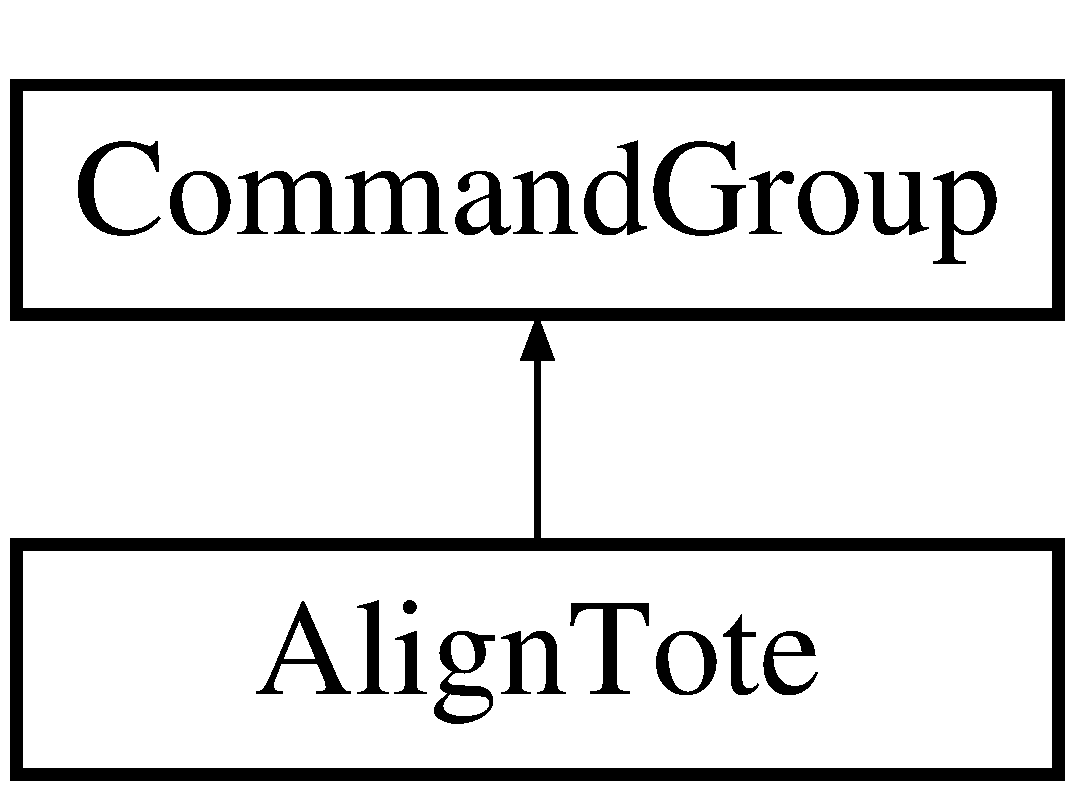
\includegraphics[height=2.000000cm]{class_align_tote}
\end{center}
\end{figure}


The documentation for this class was generated from the following files\+:\begin{DoxyCompactItemize}
\item 
Cyclophosphamide/src/\+Commands/\+Tote\+Lifting/Align\+Tote.\+h\item 
Cyclophosphamide/src/\+Commands/\+Tote\+Lifting/Align\+Tote.\+cpp\end{DoxyCompactItemize}

\hypertarget{class_analog_range_i_o_button}{}\section{Analog\+Range\+I\+O\+Button Class Reference}
\label{class_analog_range_i_o_button}\index{Analog\+Range\+I\+O\+Button@{Analog\+Range\+I\+O\+Button}}
Inheritance diagram for Analog\+Range\+I\+O\+Button\+:\begin{figure}[H]
\begin{center}
\leavevmode
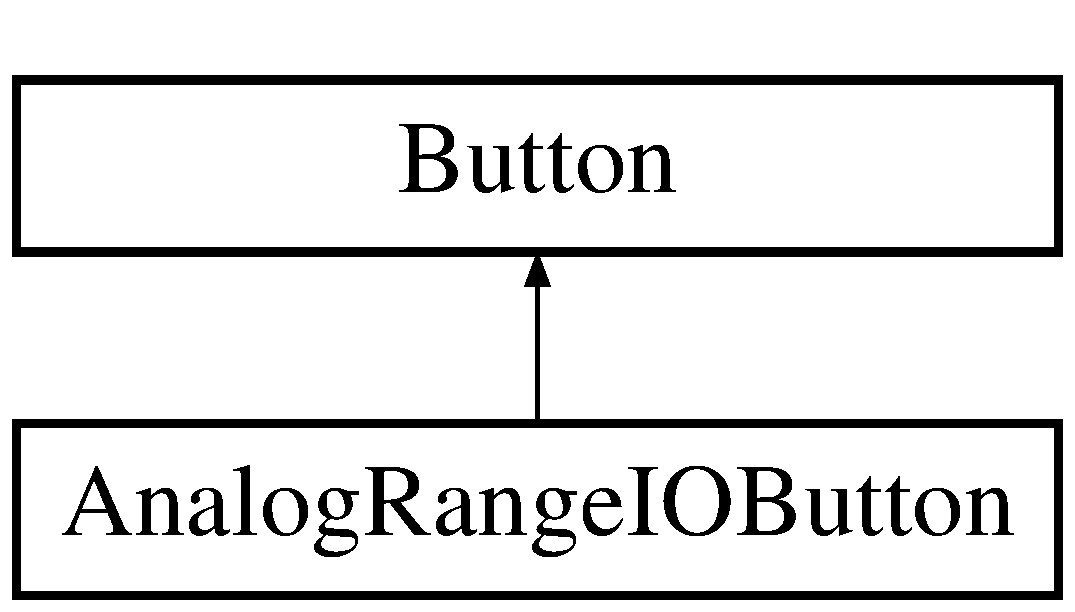
\includegraphics[height=2.000000cm]{class_analog_range_i_o_button}
\end{center}
\end{figure}
\subsection*{Public Member Functions}
\begin{DoxyCompactItemize}
\item 
\hyperlink{class_analog_range_i_o_button_ad99b0723a6b5754b442b8112c11f6197}{Analog\+Range\+I\+O\+Button} (int port, Joystick\+::\+Axis\+Type axis, double low\+Threshold, double high\+Threshold)
\begin{DoxyCompactList}\small\item\em Creates on/off states for buttons that have varying analog states. \end{DoxyCompactList}\item 
\hypertarget{class_analog_range_i_o_button_aadd957fdd7b12f3f3a8dbe5a918400c1}{}virtual bool {\bfseries Get} ()\label{class_analog_range_i_o_button_aadd957fdd7b12f3f3a8dbe5a918400c1}

\end{DoxyCompactItemize}


\subsection{Constructor \& Destructor Documentation}
\hypertarget{class_analog_range_i_o_button_ad99b0723a6b5754b442b8112c11f6197}{}\index{Analog\+Range\+I\+O\+Button@{Analog\+Range\+I\+O\+Button}!Analog\+Range\+I\+O\+Button@{Analog\+Range\+I\+O\+Button}}
\index{Analog\+Range\+I\+O\+Button@{Analog\+Range\+I\+O\+Button}!Analog\+Range\+I\+O\+Button@{Analog\+Range\+I\+O\+Button}}
\subsubsection[{Analog\+Range\+I\+O\+Button}]{\setlength{\rightskip}{0pt plus 5cm}Analog\+Range\+I\+O\+Button\+::\+Analog\+Range\+I\+O\+Button (
\begin{DoxyParamCaption}
\item[{int}]{port, }
\item[{Joystick\+::\+Axis\+Type}]{axis, }
\item[{double}]{low\+Threshold, }
\item[{double}]{high\+Threshold}
\end{DoxyParamCaption}
)}\label{class_analog_range_i_o_button_ad99b0723a6b5754b442b8112c11f6197}


Creates on/off states for buttons that have varying analog states. 


\begin{DoxyParams}{Parameters}
{\em port} & \\
\hline
{\em low\+Threshold} & \\
\hline
{\em high\+Threshold} & \\
\hline
\end{DoxyParams}


The documentation for this class was generated from the following files\+:\begin{DoxyCompactItemize}
\item 
Cyclophosphamide/src/utilities/Analog\+Range\+I\+O\+Button.\+h\item 
Cyclophosphamide/src/utilities/Analog\+Range\+I\+O\+Button.\+cpp\end{DoxyCompactItemize}

\hypertarget{class_auto_can_grabber}{}\section{Auto\+Can\+Grabber Class Reference}
\label{class_auto_can_grabber}\index{Auto\+Can\+Grabber@{Auto\+Can\+Grabber}}
Inheritance diagram for Auto\+Can\+Grabber\+:\begin{figure}[H]
\begin{center}
\leavevmode
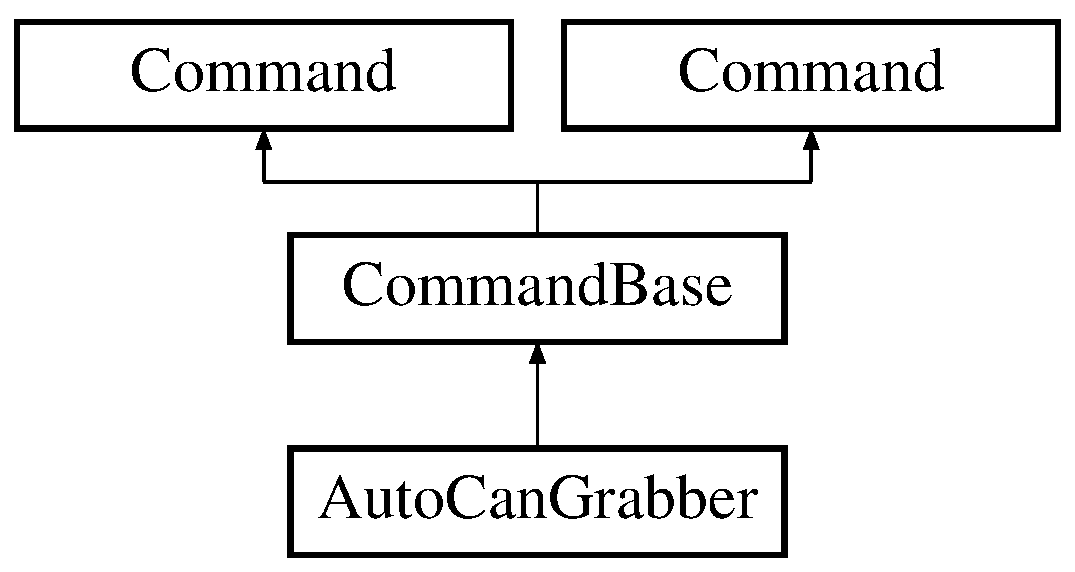
\includegraphics[height=3.000000cm]{class_auto_can_grabber}
\end{center}
\end{figure}
\subsection*{Public Member Functions}
\begin{DoxyCompactItemize}
\item 
\hypertarget{class_auto_can_grabber_a9ceccca06bb2ec22c4b995f46c36d0b7}{}{\bfseries Auto\+Can\+Grabber} (bool down)\label{class_auto_can_grabber_a9ceccca06bb2ec22c4b995f46c36d0b7}

\item 
\hypertarget{class_auto_can_grabber_aaf54de7327a81718ee71104e93412ac4}{}void {\bfseries Initialize} ()\label{class_auto_can_grabber_aaf54de7327a81718ee71104e93412ac4}

\item 
\hypertarget{class_auto_can_grabber_add9cbd78fe6d9dbd3ce5f5a08d1d905d}{}void {\bfseries Execute} ()\label{class_auto_can_grabber_add9cbd78fe6d9dbd3ce5f5a08d1d905d}

\item 
\hypertarget{class_auto_can_grabber_a466f32915e9f2c65618b98fd8389b4c4}{}bool {\bfseries Is\+Finished} ()\label{class_auto_can_grabber_a466f32915e9f2c65618b98fd8389b4c4}

\item 
\hypertarget{class_auto_can_grabber_a254da544e813595bd6a6a71b340b58d5}{}void {\bfseries End} ()\label{class_auto_can_grabber_a254da544e813595bd6a6a71b340b58d5}

\item 
\hypertarget{class_auto_can_grabber_ad524843a58e67fd0ef4a522bc0bdcd33}{}void {\bfseries Interrupted} ()\label{class_auto_can_grabber_ad524843a58e67fd0ef4a522bc0bdcd33}

\end{DoxyCompactItemize}
\subsection*{Additional Inherited Members}


The documentation for this class was generated from the following files\+:\begin{DoxyCompactItemize}
\item 
Cyclophosphamide/src/\+Commands/\+Auto\+Can/Auto\+Can\+Grabber.\+h\item 
Cyclophosphamide/src/\+Commands/\+Auto\+Can/Auto\+Can\+Grabber.\+cpp\end{DoxyCompactItemize}

\hypertarget{class_auto_can_graberino}{}\section{Auto\+Can\+Graberino Class Reference}
\label{class_auto_can_graberino}\index{Auto\+Can\+Graberino@{Auto\+Can\+Graberino}}
Inheritance diagram for Auto\+Can\+Graberino\+:\begin{figure}[H]
\begin{center}
\leavevmode
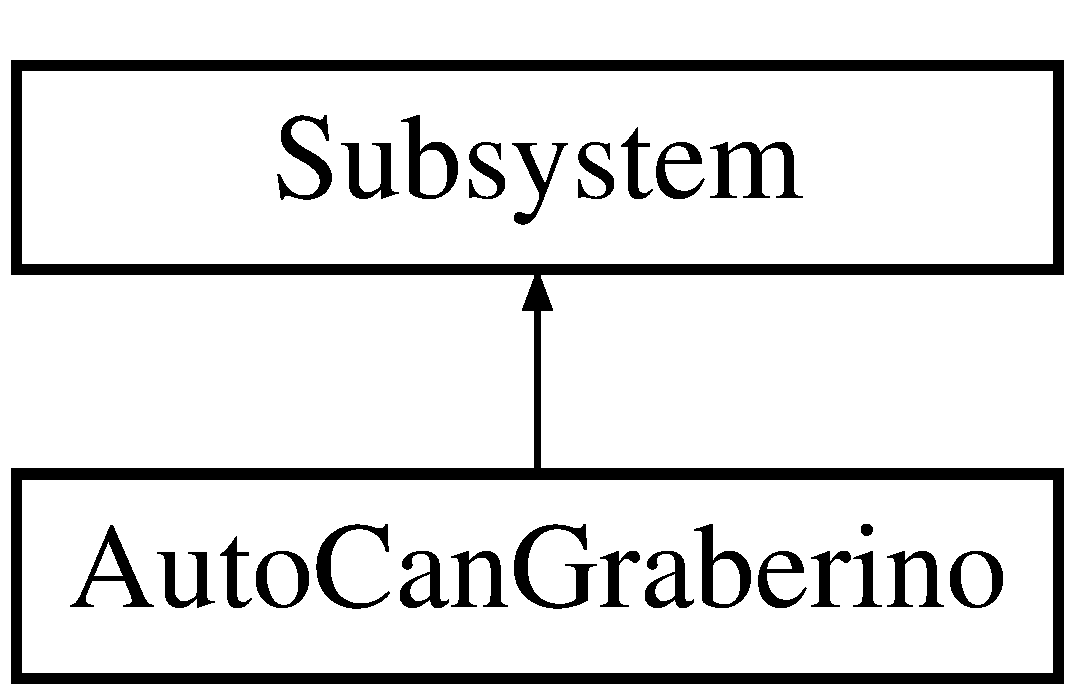
\includegraphics[height=2.000000cm]{class_auto_can_graberino}
\end{center}
\end{figure}
\subsection*{Public Types}
\begin{DoxyCompactItemize}
\item 
\hypertarget{class_auto_can_graberino_a5949187e3b8793dfe2f737909a77d83c}{}enum {\bfseries Push\+State} \{ {\bfseries up} = true, 
{\bfseries down} = false
 \}\label{class_auto_can_graberino_a5949187e3b8793dfe2f737909a77d83c}

\end{DoxyCompactItemize}
\subsection*{Public Member Functions}
\begin{DoxyCompactItemize}
\item 
\hypertarget{class_auto_can_graberino_aa7120b8f3c2d323fdc33fa39f6245cd0}{}void {\bfseries Down} ()\label{class_auto_can_graberino_aa7120b8f3c2d323fdc33fa39f6245cd0}

\item 
\hypertarget{class_auto_can_graberino_afa4cbfc5d462001da70a8d63be909d41}{}void {\bfseries Up} ()\label{class_auto_can_graberino_afa4cbfc5d462001da70a8d63be909d41}

\item 
\hypertarget{class_auto_can_graberino_a17642fc3fee2e60366272935c3c86874}{}void {\bfseries Init\+Default\+Command} ()\label{class_auto_can_graberino_a17642fc3fee2e60366272935c3c86874}

\item 
\hypertarget{class_auto_can_graberino_a699189deaac0214338b66c2ad1fe036d}{}Double\+Solenoid\+::\+Value {\bfseries get\+Value} ()\label{class_auto_can_graberino_a699189deaac0214338b66c2ad1fe036d}

\end{DoxyCompactItemize}


The documentation for this class was generated from the following files\+:\begin{DoxyCompactItemize}
\item 
Cyclophosphamide/src/\+Subsystems/Auto\+Can\+Graberino.\+h\item 
Cyclophosphamide/src/\+Subsystems/Auto\+Can\+Graberino.\+cpp\end{DoxyCompactItemize}

\hypertarget{class_autonomous}{}\section{Autonomous Class Reference}
\label{class_autonomous}\index{Autonomous@{Autonomous}}
Inheritance diagram for Autonomous\+:\begin{figure}[H]
\begin{center}
\leavevmode
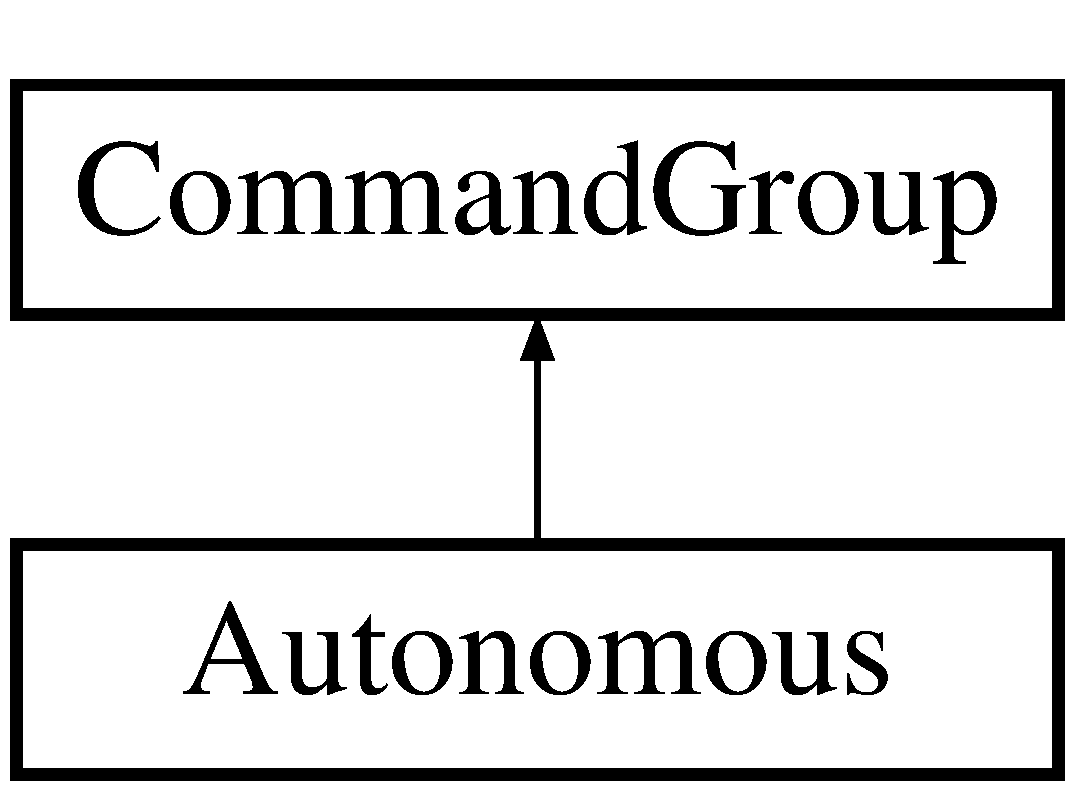
\includegraphics[height=2.000000cm]{class_autonomous}
\end{center}
\end{figure}
\subsection*{Public Member Functions}
\begin{DoxyCompactItemize}
\item 
\hypertarget{class_autonomous_a1d40e572e145f77795f0061fd2bb8773}{}{\bfseries Autonomous} (char $\ast$style)\label{class_autonomous_a1d40e572e145f77795f0061fd2bb8773}

\item 
\hypertarget{class_autonomous_a55f5b6ad9641b9335c8569586877d17e}{}{\bfseries Autonomous} (int argc, char $\ast$$\ast$argv)\label{class_autonomous_a55f5b6ad9641b9335c8569586877d17e}

\item 
\hypertarget{class_autonomous_a29e2122506fb216d8f5624e18978b66b}{}virtual void {\bfseries Initialize} ()\label{class_autonomous_a29e2122506fb216d8f5624e18978b66b}

\end{DoxyCompactItemize}
\subsection*{Static Public Member Functions}
\begin{DoxyCompactItemize}
\item 
\hypertarget{class_autonomous_a6391f5e216f820029437e351bb84ae7c}{}static \hyperlink{class_autonomous}{Autonomous} $\ast$ {\bfseries create\+Drive\+Distance} (float distance, Best\+Drive\+::\+Direction direction)\label{class_autonomous_a6391f5e216f820029437e351bb84ae7c}

\item 
\hypertarget{class_autonomous_a500383605a081ceed65af68d7be3345d}{}static \hyperlink{class_autonomous}{Autonomous} $\ast$ {\bfseries create\+Drive\+Duration} (float duration, float heading)\label{class_autonomous_a500383605a081ceed65af68d7be3345d}

\item 
\hypertarget{class_autonomous_a43817961cc483af7d727a19dbb997484}{}static \hyperlink{class_autonomous}{Autonomous} $\ast$ {\bfseries create\+Turn\+To} (double target\+Angle)\label{class_autonomous_a43817961cc483af7d727a19dbb997484}

\item 
\hypertarget{class_autonomous_a5d1c89c581c7bb894a8d89df1e1d3ba4}{}static \hyperlink{class_autonomous}{Autonomous} $\ast$ {\bfseries create\+Triple\+Tote} ()\label{class_autonomous_a5d1c89c581c7bb894a8d89df1e1d3ba4}

\item 
\hypertarget{class_autonomous_af17ae791956f3bc069cdf89f197ecfc0}{}static \hyperlink{class_autonomous}{Autonomous} $\ast$ {\bfseries create\+Turning\+Triple\+Tote} ()\label{class_autonomous_af17ae791956f3bc069cdf89f197ecfc0}

\item 
\hypertarget{class_autonomous_ac8b0ffd5e3720924016111dc78491152}{}static \hyperlink{class_autonomous}{Autonomous} $\ast$ {\bfseries create\+Start\+With\+Can} ()\label{class_autonomous_ac8b0ffd5e3720924016111dc78491152}

\item 
\hypertarget{class_autonomous_a881241af00a09552049999e698948091}{}static \hyperlink{class_autonomous}{Autonomous} $\ast$ {\bfseries create\+Simple\+Drive\+Forward} ()\label{class_autonomous_a881241af00a09552049999e698948091}

\end{DoxyCompactItemize}


The documentation for this class was generated from the following files\+:\begin{DoxyCompactItemize}
\item 
Cyclophosphamide/src/\+Commands/\+Autonomous/Autonomous.\+h\item 
Cyclophosphamide/src/\+Commands/\+Autonomous/Autonomous.\+cpp\item 
Cyclophosphamide/src/\+Commands/\+Autonomous/Drive\+Distance.\+cpp\item 
Cyclophosphamide/src/\+Commands/\+Autonomous/Drive\+Duration.\+cpp\item 
Cyclophosphamide/src/\+Commands/\+Autonomous/Simple\+Drive\+Forward.\+cpp\item 
Cyclophosphamide/src/\+Commands/\+Autonomous/Start\+With\+Can.\+cpp\item 
Cyclophosphamide/src/\+Commands/\+Autonomous/Turn\+Command.\+cpp\item 
Cyclophosphamide/src/\+Commands/\+Autonomous/Turning\+Triple\+Tote.\+cpp\end{DoxyCompactItemize}

\hypertarget{class_best_drive}{}\section{Best\+Drive Class Reference}
\label{class_best_drive}\index{Best\+Drive@{Best\+Drive}}
Inheritance diagram for Best\+Drive\+:\begin{figure}[H]
\begin{center}
\leavevmode
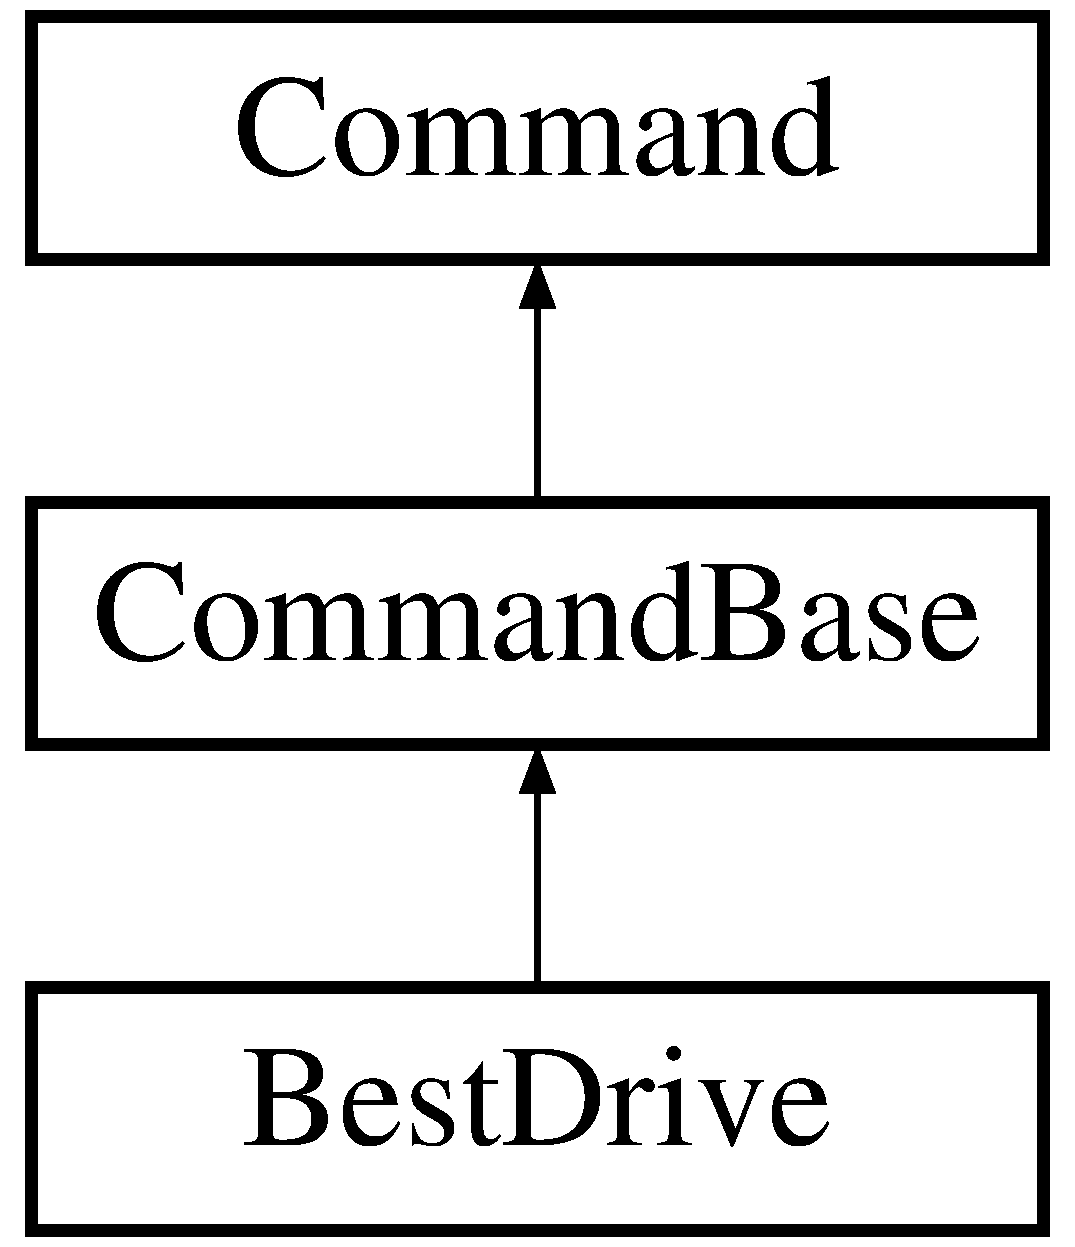
\includegraphics[height=3.000000cm]{class_best_drive}
\end{center}
\end{figure}
\subsection*{Public Types}
\begin{DoxyCompactItemize}
\item 
\hypertarget{class_best_drive_a0649c88785769dedd5adbac478aa761a}{}enum {\bfseries Direction} \{ {\bfseries forward}, 
{\bfseries backward}, 
{\bfseries left}, 
{\bfseries right}
 \}\label{class_best_drive_a0649c88785769dedd5adbac478aa761a}

\end{DoxyCompactItemize}
\subsection*{Public Member Functions}
\begin{DoxyCompactItemize}
\item 
\hypertarget{class_best_drive_aa1ddc3e387fa0eed5941a52dcb4f5dd6}{}{\bfseries Best\+Drive} (float distance, Direction direction)\label{class_best_drive_aa1ddc3e387fa0eed5941a52dcb4f5dd6}

\item 
\hypertarget{class_best_drive_a1837e8ae6f533835175e3014ec959d9b}{}void {\bfseries Initialize} ()\label{class_best_drive_a1837e8ae6f533835175e3014ec959d9b}

\item 
\hypertarget{class_best_drive_a5d3e4b21cfcb5a719a4f3aa347c24784}{}void {\bfseries Execute} ()\label{class_best_drive_a5d3e4b21cfcb5a719a4f3aa347c24784}

\item 
\hypertarget{class_best_drive_a0ddfa6d57679ca2709ff751019102229}{}bool {\bfseries Is\+Finished} ()\label{class_best_drive_a0ddfa6d57679ca2709ff751019102229}

\item 
\hypertarget{class_best_drive_a6aa048014fa7605362f58eb8d92031cc}{}void {\bfseries End} ()\label{class_best_drive_a6aa048014fa7605362f58eb8d92031cc}

\item 
\hypertarget{class_best_drive_ab78dba87be3312f9d3c5327a74b9a75d}{}void {\bfseries Interrupted} ()\label{class_best_drive_ab78dba87be3312f9d3c5327a74b9a75d}

\end{DoxyCompactItemize}
\subsection*{Additional Inherited Members}


The documentation for this class was generated from the following files\+:\begin{DoxyCompactItemize}
\item 
Cyclophosphamide/src/\+Commands/\+Automatic/Best\+Drive.\+h\item 
Cyclophosphamide/src/\+Commands/\+Automatic/Best\+Drive.\+cpp\end{DoxyCompactItemize}

\hypertarget{class_can_collecterino}{}\section{Can\+Collecterino Class Reference}
\label{class_can_collecterino}\index{Can\+Collecterino@{Can\+Collecterino}}


{\ttfamily \#include $<$Can\+Collecterino.\+h$>$}

Inheritance diagram for Can\+Collecterino\+:\begin{figure}[H]
\begin{center}
\leavevmode
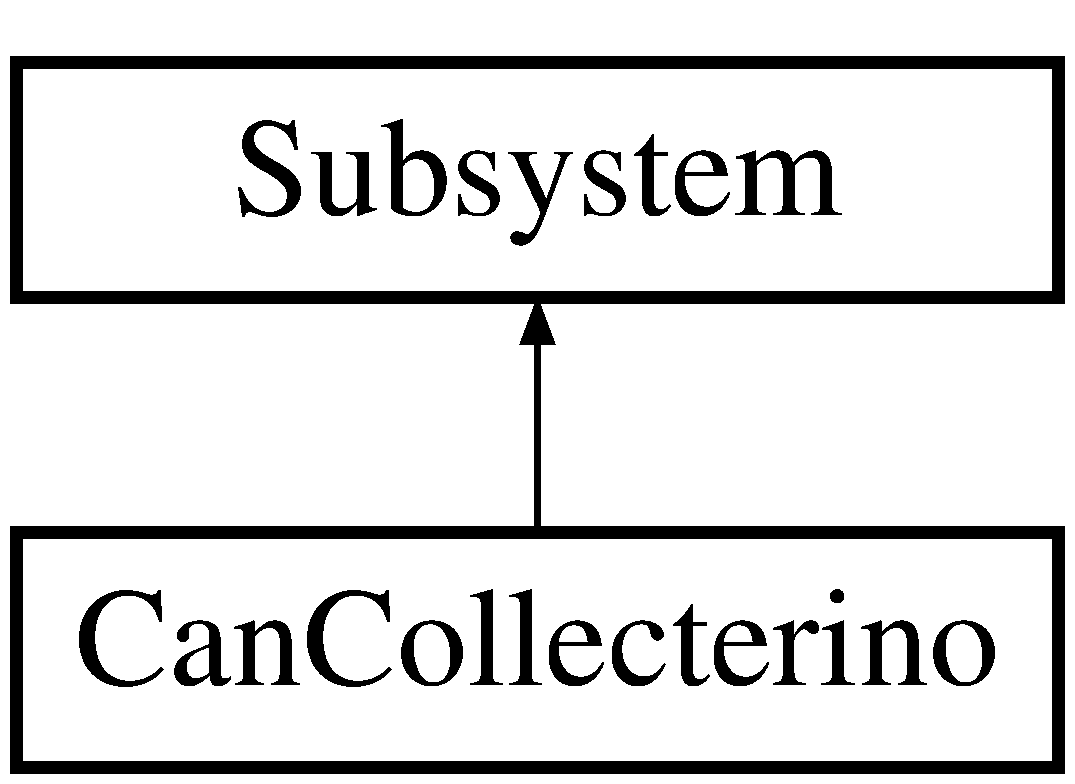
\includegraphics[height=2.000000cm]{class_can_collecterino}
\end{center}
\end{figure}
\subsection*{Public Member Functions}
\begin{DoxyCompactItemize}
\item 
\hypertarget{class_can_collecterino_a25f7c7e5898c30724ae1bf47a7b38e10}{}void {\bfseries Init\+Default\+Command} ()\label{class_can_collecterino_a25f7c7e5898c30724ae1bf47a7b38e10}

\item 
\hypertarget{class_can_collecterino_a2335715a8e197011cfd483302011f8e8}{}void {\bfseries set\+Arms} (float value)\label{class_can_collecterino_a2335715a8e197011cfd483302011f8e8}

\item 
\hypertarget{class_can_collecterino_a60a79346dbaf1d987aba9ef2c950afb4}{}void {\bfseries disable\+Arms} ()\label{class_can_collecterino_a60a79346dbaf1d987aba9ef2c950afb4}

\item 
\hypertarget{class_can_collecterino_adc9e17256b4a00fede2ed7762aeb03c6}{}bool {\bfseries arms\+Within\+Bounds} ()\label{class_can_collecterino_adc9e17256b4a00fede2ed7762aeb03c6}

\item 
\hypertarget{class_can_collecterino_afceae0f9c91f4301137d8e2904e11ae8}{}void {\bfseries brake\+Arms} (bool brake)\label{class_can_collecterino_afceae0f9c91f4301137d8e2904e11ae8}

\item 
\hypertarget{class_can_collecterino_a0eff9a330a430c233b5ae7f72ec13d8b}{}Analog\+Input $\ast$ {\bfseries get\+Lift\+Pot} ()\label{class_can_collecterino_a0eff9a330a430c233b5ae7f72ec13d8b}

\item 
\hypertarget{class_can_collecterino_ad955ee01debe943bf9e749a5bee0b9ef}{}P\+I\+D\+Controller $\ast$ {\bfseries get\+Arm\+P\+I\+D} ()\label{class_can_collecterino_ad955ee01debe943bf9e749a5bee0b9ef}

\item 
\hypertarget{class_can_collecterino_a923a76084bdec56e4e7ad7f8da0842ad}{}bool {\bfseries get\+Toggle\+Arms} ()\label{class_can_collecterino_a923a76084bdec56e4e7ad7f8da0842ad}

\item 
\hypertarget{class_can_collecterino_a62ef9056b5efd3bb50a1bc5fd60b1b05}{}void {\bfseries do\+The\+Toggle\+Arms} ()\label{class_can_collecterino_a62ef9056b5efd3bb50a1bc5fd60b1b05}

\item 
\hypertarget{class_can_collecterino_a66118988ad6367103a511e7bbf0a8a52}{}void {\bfseries get\+Dat\+Status} ()\label{class_can_collecterino_a66118988ad6367103a511e7bbf0a8a52}

\item 
\hypertarget{class_can_collecterino_a6591ee572d092a4015a7351dfe41fab8}{}double {\bfseries get\+Setpoint} ()\label{class_can_collecterino_a6591ee572d092a4015a7351dfe41fab8}

\end{DoxyCompactItemize}


\subsection{Detailed Description}
Motor arms raise up/down Arm P\+I\+D controls the arms up and down. can sensor Pneumatics (double solenoid) wrist open and close to collect the recycle can. 

The documentation for this class was generated from the following files\+:\begin{DoxyCompactItemize}
\item 
Cyclophosphamide/src/\+Subsystems/Can\+Collecterino.\+h\item 
Cyclophosphamide/src/\+Subsystems/Can\+Collecterino.\+cpp\end{DoxyCompactItemize}

\hypertarget{class_can_intakerino}{}\section{Can\+Intakerino Class Reference}
\label{class_can_intakerino}\index{Can\+Intakerino@{Can\+Intakerino}}


{\ttfamily \#include $<$Can\+Intakerino.\+h$>$}

Inheritance diagram for Can\+Intakerino\+:\begin{figure}[H]
\begin{center}
\leavevmode
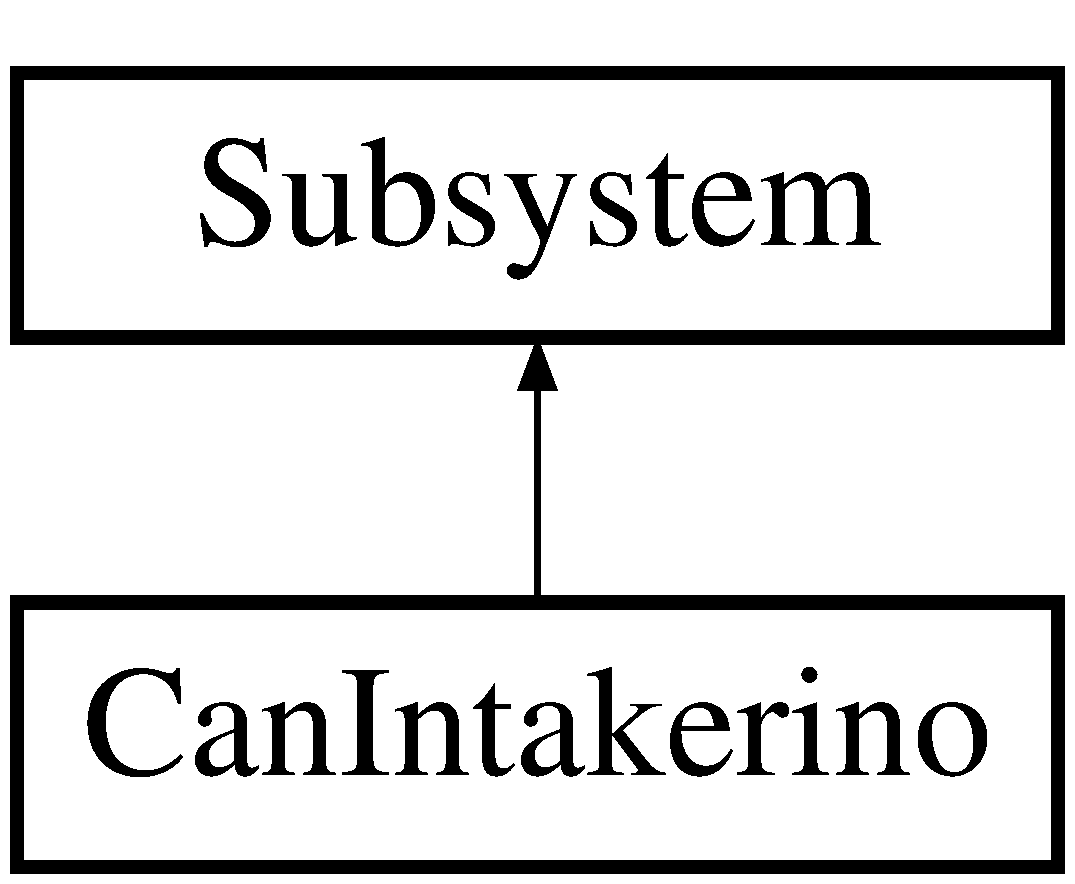
\includegraphics[height=2.000000cm]{class_can_intakerino}
\end{center}
\end{figure}
\subsection*{Public Member Functions}
\begin{DoxyCompactItemize}
\item 
\hypertarget{class_can_intakerino_a439ef3fdbc09691bdeb8db5e3f632a17}{}void {\bfseries set\+Grab} (float value)\label{class_can_intakerino_a439ef3fdbc09691bdeb8db5e3f632a17}

\end{DoxyCompactItemize}


\subsection{Detailed Description}
2 motors to run the wheels, and intake/expell the can.

the wheels spin to intake or expell the recycle bin. 

The documentation for this class was generated from the following files\+:\begin{DoxyCompactItemize}
\item 
Cyclophosphamide/src/\+Subsystems/Can\+Intakerino.\+h\item 
Cyclophosphamide/src/\+Subsystems/Can\+Intakerino.\+cpp\end{DoxyCompactItemize}

\hypertarget{class_can_to_craaaw_transfer}{}\section{Can\+To\+Craaaw\+Transfer Class Reference}
\label{class_can_to_craaaw_transfer}\index{Can\+To\+Craaaw\+Transfer@{Can\+To\+Craaaw\+Transfer}}
Inheritance diagram for Can\+To\+Craaaw\+Transfer\+:\begin{figure}[H]
\begin{center}
\leavevmode
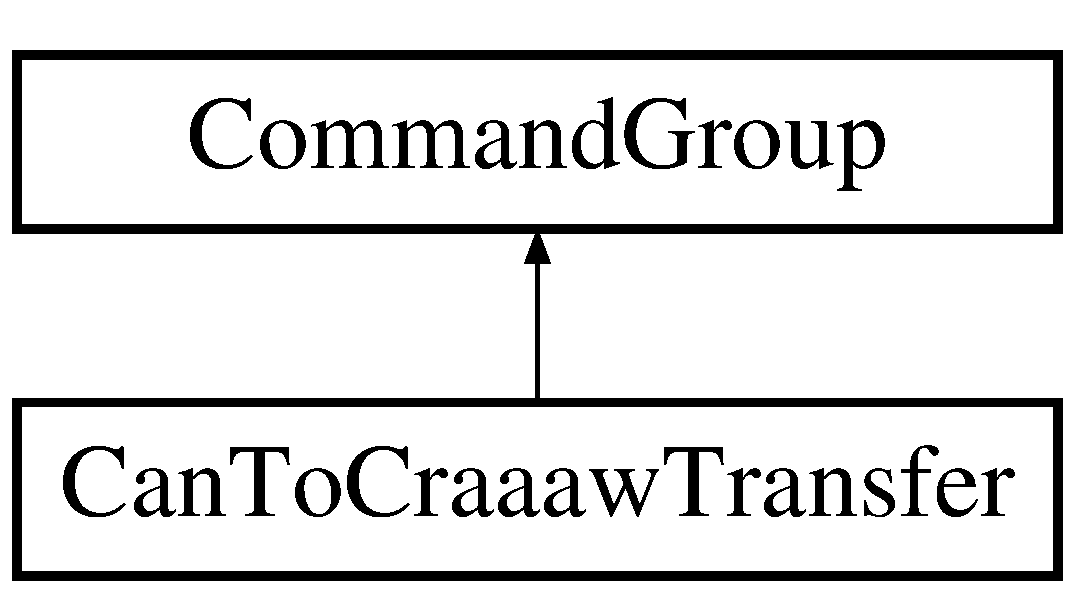
\includegraphics[height=2.000000cm]{class_can_to_craaaw_transfer}
\end{center}
\end{figure}


The documentation for this class was generated from the following files\+:\begin{DoxyCompactItemize}
\item 
Cyclophosphamide/src/\+Commands/\+Can\+Collecterino/Can\+To\+Craaaw\+Transfer.\+h\item 
Cyclophosphamide/src/\+Commands/\+Can\+Collecterino/Can\+To\+Craaaw\+Transfer.\+cpp\end{DoxyCompactItemize}

\hypertarget{class_can_wristerino}{}\section{Can\+Wristerino Class Reference}
\label{class_can_wristerino}\index{Can\+Wristerino@{Can\+Wristerino}}
Inheritance diagram for Can\+Wristerino\+:\begin{figure}[H]
\begin{center}
\leavevmode
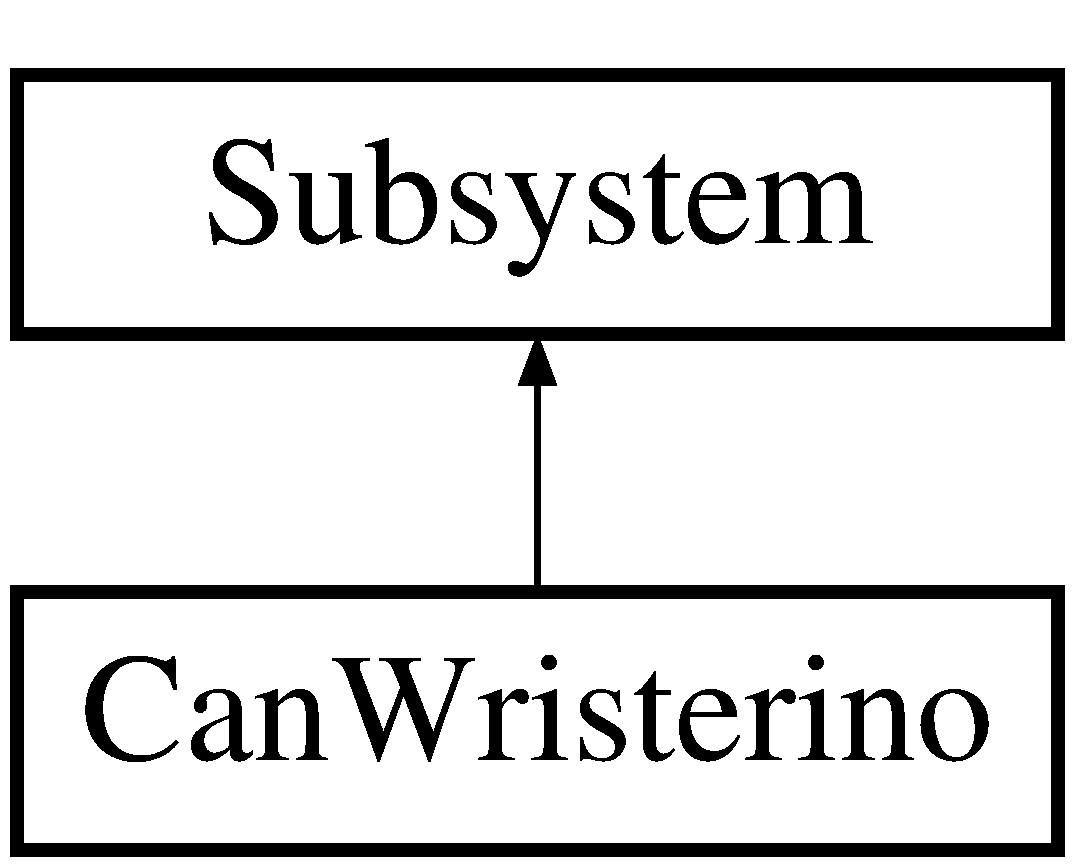
\includegraphics[height=2.000000cm]{class_can_wristerino}
\end{center}
\end{figure}
\subsection*{Public Member Functions}
\begin{DoxyCompactItemize}
\item 
\hypertarget{class_can_wristerino_a59e4a4005b747d4c3a7965158f84ba0b}{}void {\bfseries Init\+Default\+Command} ()\label{class_can_wristerino_a59e4a4005b747d4c3a7965158f84ba0b}

\item 
\hypertarget{class_can_wristerino_aae53b74938aa3c606d2aa07f8da93b86}{}void {\bfseries set\+Wrist} (Double\+Solenoid\+::\+Value value)\label{class_can_wristerino_aae53b74938aa3c606d2aa07f8da93b86}

\item 
\hypertarget{class_can_wristerino_a6555d37a0301532854a85c0a4419ee5e}{}bool {\bfseries get\+Wrist\+Toggle} ()\label{class_can_wristerino_a6555d37a0301532854a85c0a4419ee5e}

\item 
\hypertarget{class_can_wristerino_a7a7aa32ed931d705aedecfda346c77c0}{}void {\bfseries do\+The\+Toggle\+Wrist} ()\label{class_can_wristerino_a7a7aa32ed931d705aedecfda346c77c0}

\end{DoxyCompactItemize}


The documentation for this class was generated from the following files\+:\begin{DoxyCompactItemize}
\item 
Cyclophosphamide/src/\+Subsystems/Can\+Wristerino.\+h\item 
Cyclophosphamide/src/\+Subsystems/Can\+Wristerino.\+cpp\end{DoxyCompactItemize}

\hypertarget{class_collect}{}\section{Collect Class Reference}
\label{class_collect}\index{Collect@{Collect}}


{\ttfamily \#include $<$Collect.\+h$>$}

Inheritance diagram for Collect\+:\begin{figure}[H]
\begin{center}
\leavevmode
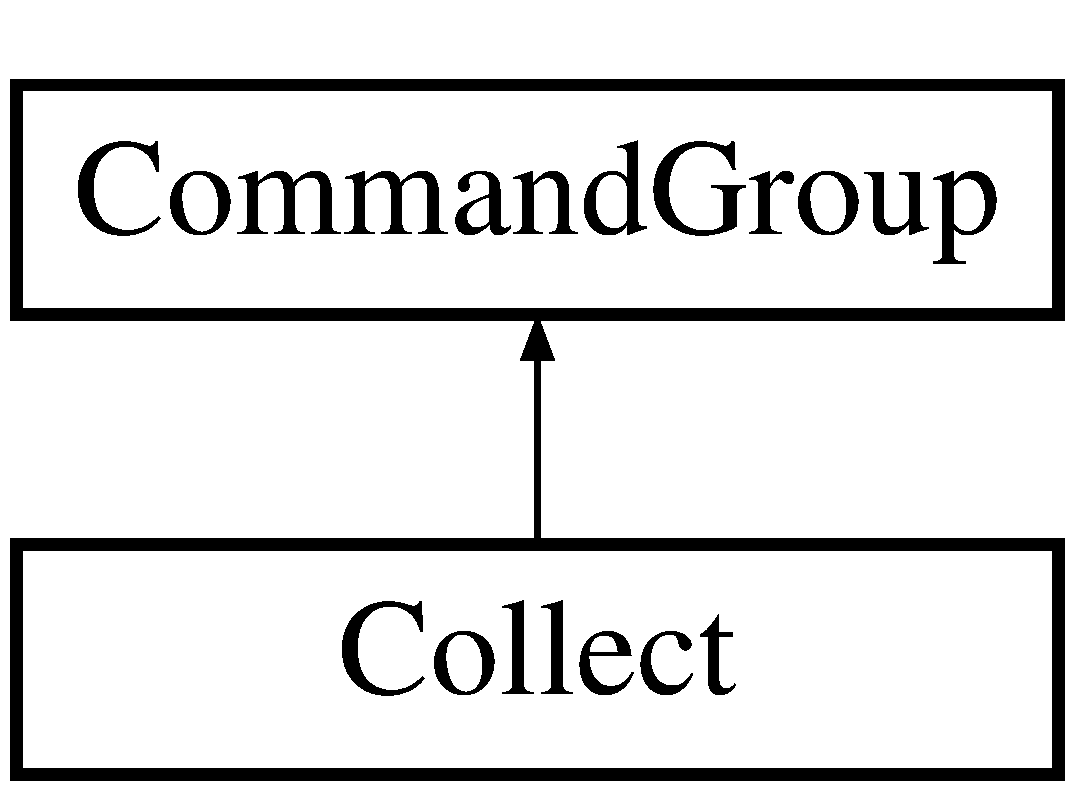
\includegraphics[height=2.000000cm]{class_collect}
\end{center}
\end{figure}
\subsection*{Public Member Functions}
\begin{DoxyCompactItemize}
\item 
\hypertarget{class_collect_a2c5b2bb92dd92765c4f83e37da5eb510}{}{\bfseries Collect} (Induct\+::\+State direction=Induct\+::forward, Move\+Wrist\+::\+State state=Move\+Wrist\+::close)\label{class_collect_a2c5b2bb92dd92765c4f83e37da5eb510}

\end{DoxyCompactItemize}


\subsection{Detailed Description}
Toggles the wrists and induct so that a can can be collected 

The documentation for this class was generated from the following files\+:\begin{DoxyCompactItemize}
\item 
Cyclophosphamide/src/\+Commands/\+Can\+Collecterino/Collect.\+h\item 
Cyclophosphamide/src/\+Commands/\+Can\+Collecterino/Collect.\+cpp\end{DoxyCompactItemize}

\hypertarget{class_command_base}{}\section{Command\+Base Class Reference}
\label{class_command_base}\index{Command\+Base@{Command\+Base}}
Inheritance diagram for Command\+Base\+:\begin{figure}[H]
\begin{center}
\leavevmode
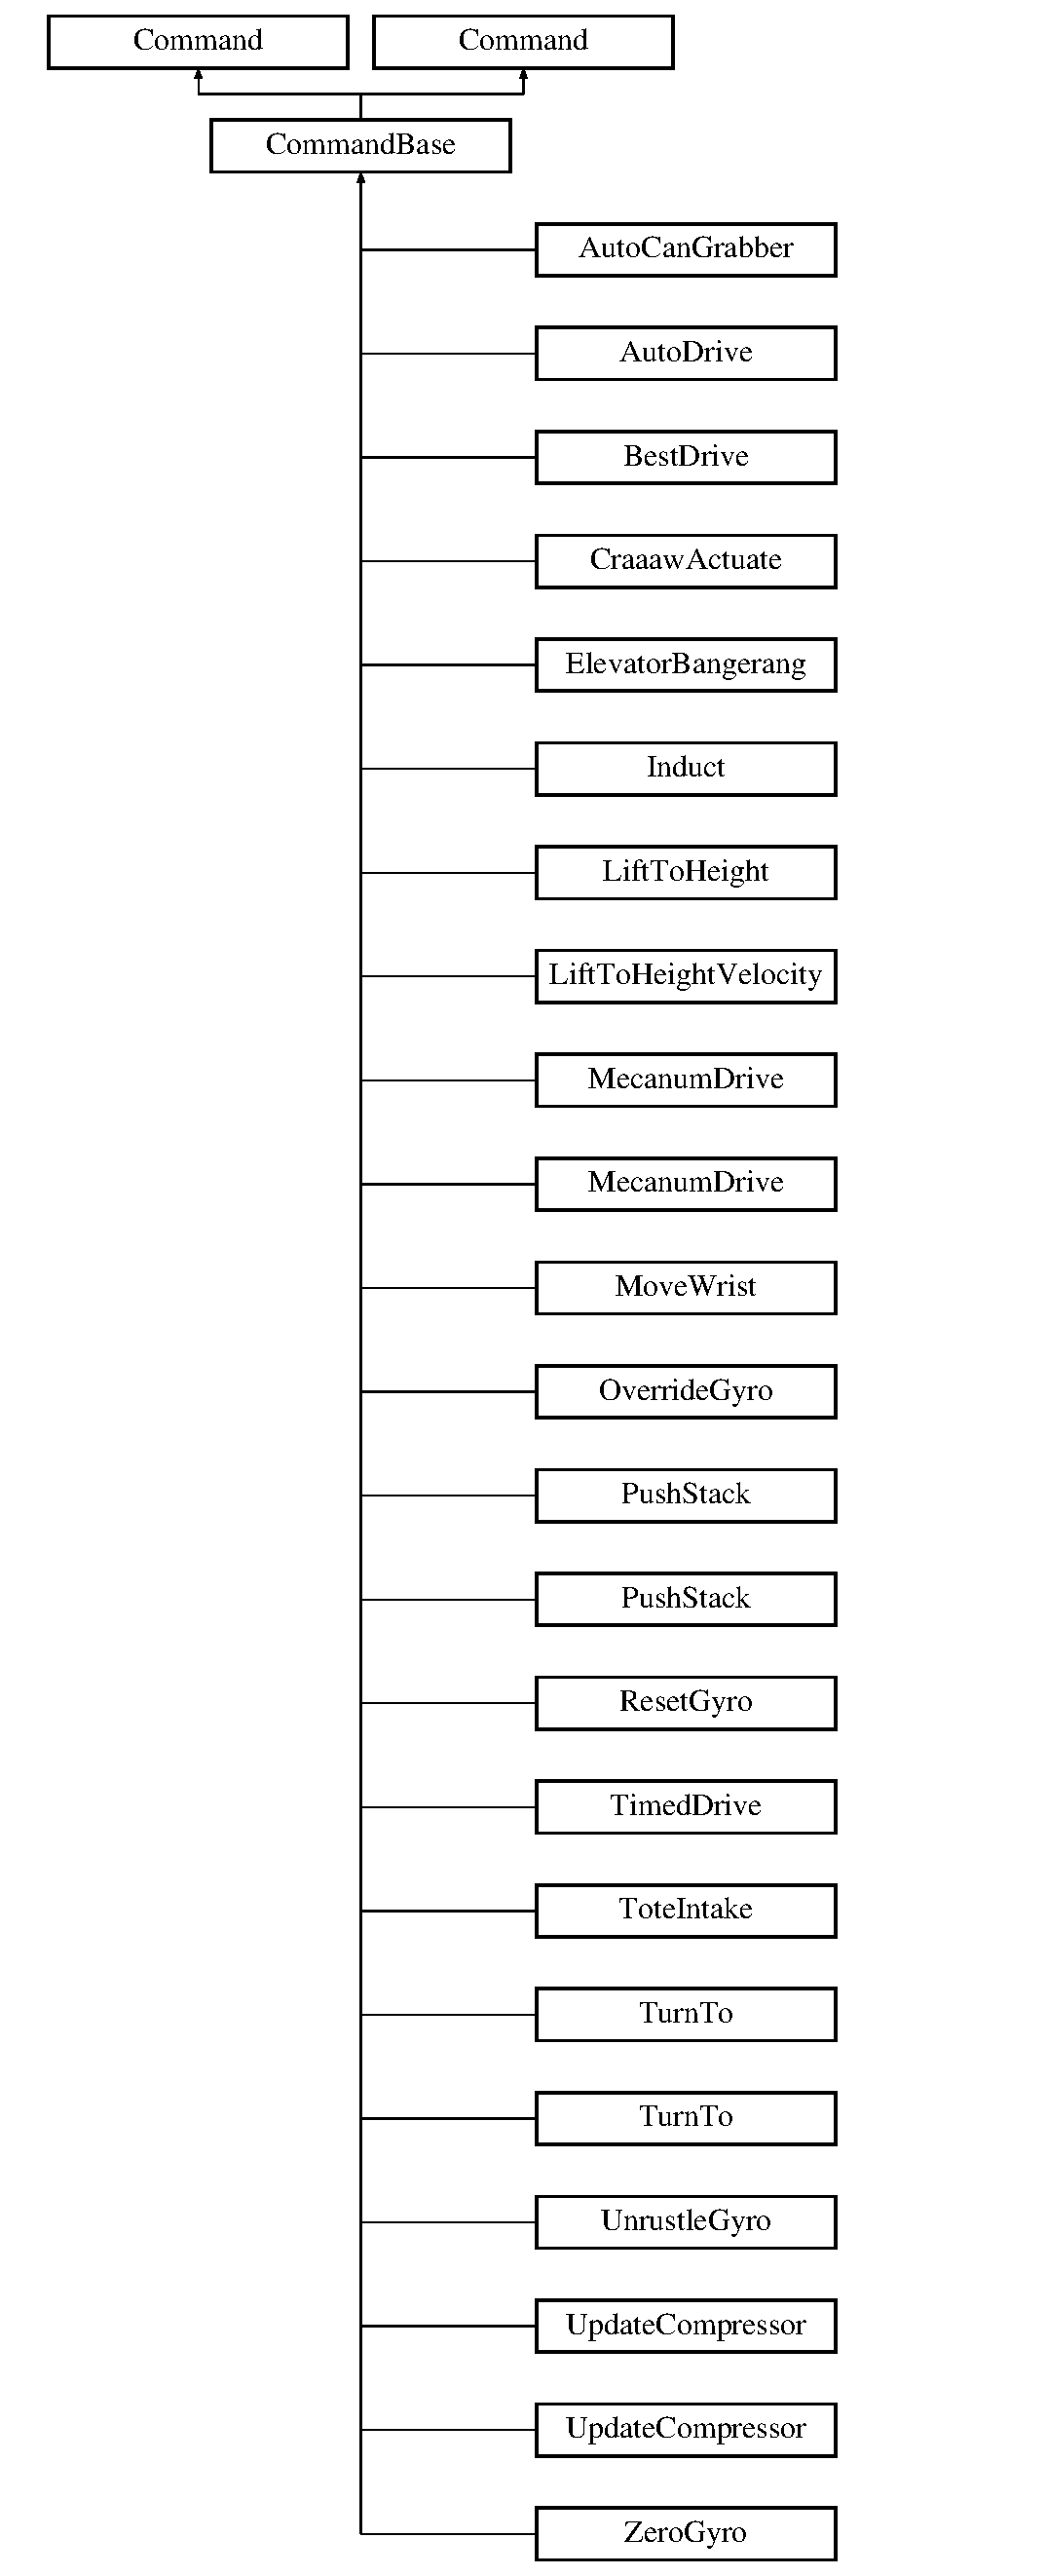
\includegraphics[height=12.000000cm]{class_command_base}
\end{center}
\end{figure}
\subsection*{Public Member Functions}
\begin{DoxyCompactItemize}
\item 
\hypertarget{class_command_base_a41d5830644dae72497af945aafac9176}{}{\bfseries Command\+Base} (char const $\ast$name)\label{class_command_base_a41d5830644dae72497af945aafac9176}

\end{DoxyCompactItemize}
\subsection*{Static Public Member Functions}
\begin{DoxyCompactItemize}
\item 
\hypertarget{class_command_base_a4dbfcd3b6ae92d752bc36a29dd1e1a5a}{}static void {\bfseries init} ()\label{class_command_base_a4dbfcd3b6ae92d752bc36a29dd1e1a5a}

\end{DoxyCompactItemize}
\subsection*{Static Public Attributes}
\begin{DoxyCompactItemize}
\item 
\hypertarget{class_command_base_aa28ad51d4be3179d9a50932b3232292e}{}static \hyperlink{class_drive_bae}{Drive\+Bae} $\ast$ {\bfseries drive\+Bae} = N\+U\+L\+L\label{class_command_base_aa28ad51d4be3179d9a50932b3232292e}

\item 
\hypertarget{class_command_base_af6de215cde5d61baa455454d6811990e}{}static \hyperlink{class_craaaw}{Craaaw} $\ast$ {\bfseries craaaw} = N\+U\+L\+L\label{class_command_base_af6de215cde5d61baa455454d6811990e}

\item 
\hypertarget{class_command_base_a1d3d0334b1085bc85f88c3ea73777a14}{}static \hyperlink{class_can_collecterino}{Can\+Collecterino} $\ast$ {\bfseries can\+Collecterino} = N\+U\+L\+L\label{class_command_base_a1d3d0334b1085bc85f88c3ea73777a14}

\item 
\hypertarget{class_command_base_ac364637c399a5b4e6db01113ae9a230f}{}static \hyperlink{class_can_wristerino}{Can\+Wristerino} $\ast$ {\bfseries can\+Wristerino} = N\+U\+L\+L\label{class_command_base_ac364637c399a5b4e6db01113ae9a230f}

\item 
\hypertarget{class_command_base_af9fc2f84b79ccdf1200e915a7d5a58aa}{}static \hyperlink{class_can_intakerino}{Can\+Intakerino} $\ast$ {\bfseries can\+Intakerino} = N\+U\+L\+L\label{class_command_base_af9fc2f84b79ccdf1200e915a7d5a58aa}

\item 
\hypertarget{class_command_base_a7afb80d21b6b8376ef0de8e26e9fb049}{}static \hyperlink{class_tote_intakerino}{Tote\+Intakerino} $\ast$ {\bfseries tote\+Intakerino} = N\+U\+L\+L\label{class_command_base_a7afb80d21b6b8376ef0de8e26e9fb049}

\item 
\hypertarget{class_command_base_aa4a4fb0c3dedaa455327bb3e4217f656}{}static \hyperlink{class_tote_lifterino}{Tote\+Lifterino} $\ast$ {\bfseries tote\+Lifterino} = N\+U\+L\+L\label{class_command_base_aa4a4fb0c3dedaa455327bb3e4217f656}

\item 
\hypertarget{class_command_base_ae6807501159925367f8008fc0534eda5}{}static \hyperlink{class_o_i}{O\+I} $\ast$ {\bfseries oi} = N\+U\+L\+L\label{class_command_base_ae6807501159925367f8008fc0534eda5}

\item 
\hypertarget{class_command_base_adb07a4bff4cadca38d0b51603d65eb7e}{}static Pneumatics $\ast$ {\bfseries pneumatics} = N\+U\+L\+L\label{class_command_base_adb07a4bff4cadca38d0b51603d65eb7e}

\end{DoxyCompactItemize}


The documentation for this class was generated from the following files\+:\begin{DoxyCompactItemize}
\item 
Cyclophosphamide/src/Command\+Base.\+h\item 
Cyclophosphamide/src/Command\+Base.\+cpp\end{DoxyCompactItemize}

\hypertarget{class_craaaw}{}\section{Craaaw Class Reference}
\label{class_craaaw}\index{Craaaw@{Craaaw}}


{\ttfamily \#include $<$Craaaw.\+h$>$}

Inheritance diagram for Craaaw\+:\begin{figure}[H]
\begin{center}
\leavevmode
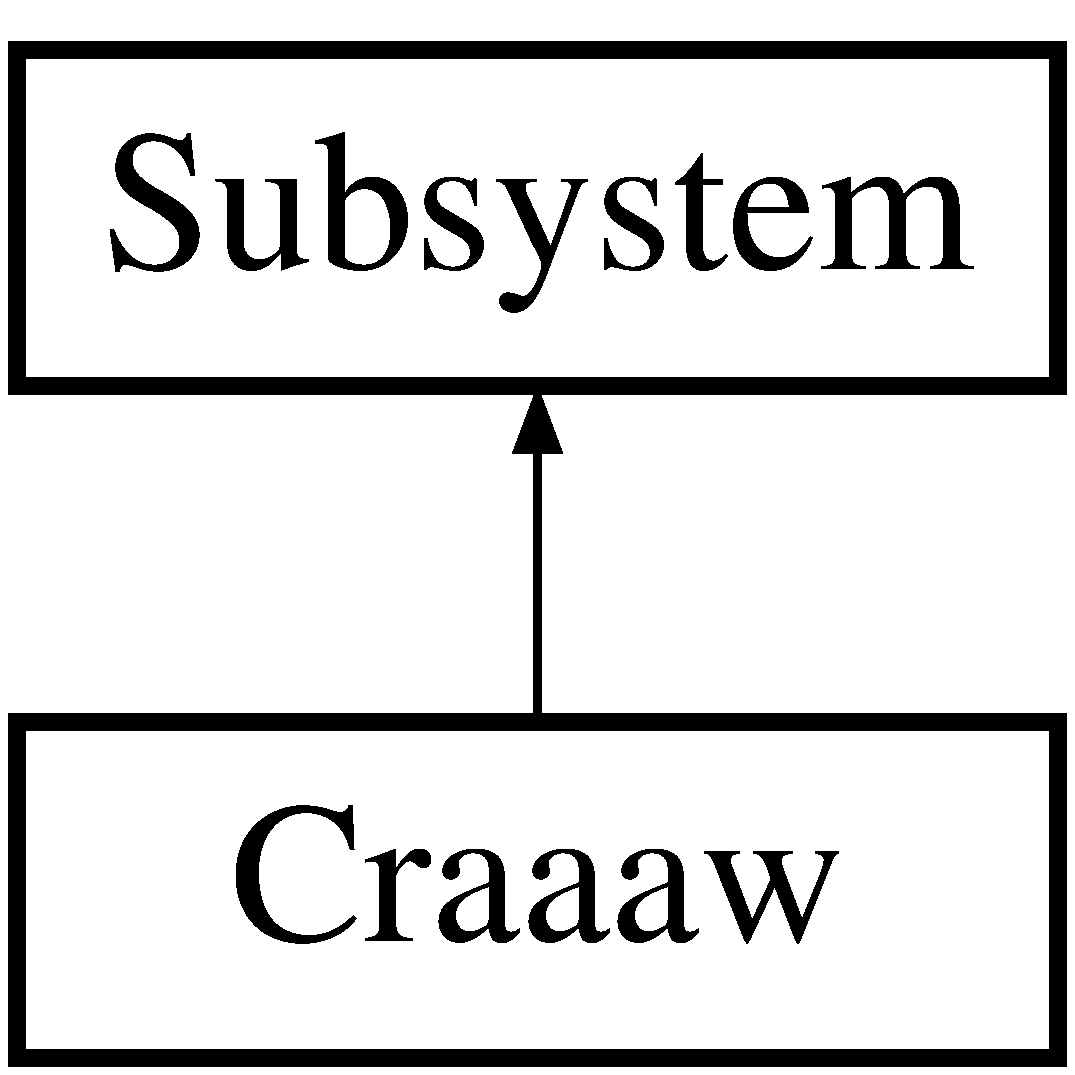
\includegraphics[height=2.000000cm]{class_craaaw}
\end{center}
\end{figure}
\subsection*{Public Member Functions}
\begin{DoxyCompactItemize}
\item 
\hypertarget{class_craaaw_ac6c9fcc66d7f9774d3f3c197f486beac}{}void {\bfseries Init\+Default\+Command} ()\label{class_craaaw_ac6c9fcc66d7f9774d3f3c197f486beac}

\item 
\hypertarget{class_craaaw_a136325b9f3185faddfa4c52961114986}{}void {\bfseries set\+Actuated} (bool actuate)\label{class_craaaw_a136325b9f3185faddfa4c52961114986}

\item 
\hypertarget{class_craaaw_a11298c00a8397de8f85ad638c6b9bea0}{}bool {\bfseries get\+Can\+Detector} ()\label{class_craaaw_a11298c00a8397de8f85ad638c6b9bea0}

\end{DoxyCompactItemize}


\subsection{Detailed Description}
pneumatics Craw, if they actuate then the claw will close the wrist. 

The documentation for this class was generated from the following files\+:\begin{DoxyCompactItemize}
\item 
Cyclophosphamide/src/\+Subsystems/Craaaw.\+h\item 
Cyclophosphamide/src/\+Subsystems/Craaaw.\+cpp\end{DoxyCompactItemize}

\hypertarget{class_craaaw_actuate}{}\section{Craaaw\+Actuate Class Reference}
\label{class_craaaw_actuate}\index{Craaaw\+Actuate@{Craaaw\+Actuate}}
Inheritance diagram for Craaaw\+Actuate\+:\begin{figure}[H]
\begin{center}
\leavevmode
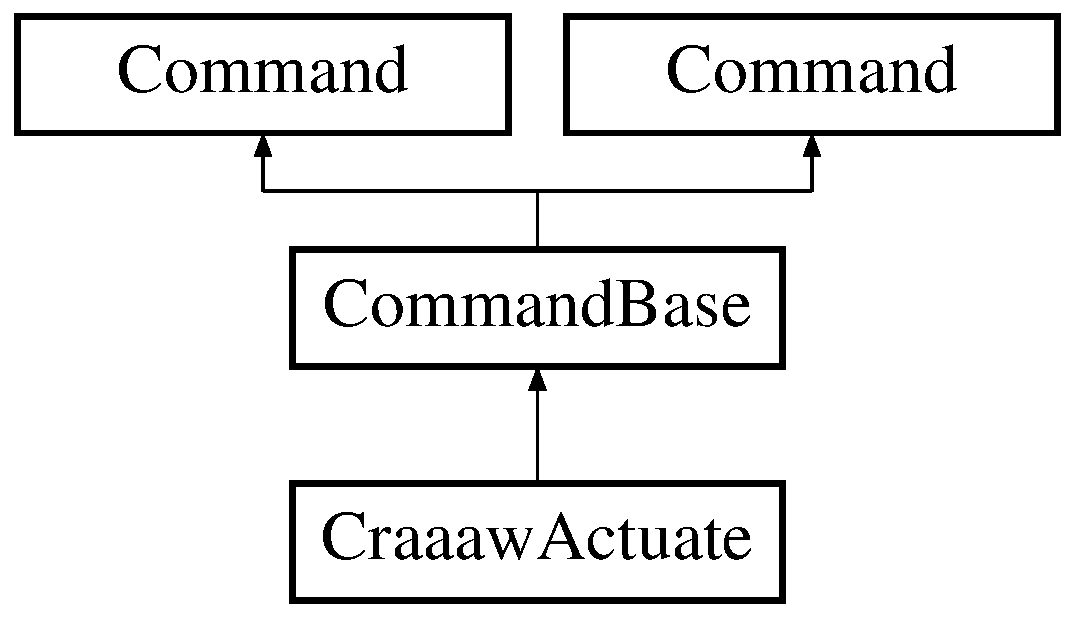
\includegraphics[height=3.000000cm]{class_craaaw_actuate}
\end{center}
\end{figure}
\subsection*{Public Member Functions}
\begin{DoxyCompactItemize}
\item 
\hypertarget{class_craaaw_actuate_a85d88e3f43f5d21138d78f9cf6aff479}{}{\bfseries Craaaw\+Actuate} (bool wait\+For\+Input)\label{class_craaaw_actuate_a85d88e3f43f5d21138d78f9cf6aff479}

\item 
\hypertarget{class_craaaw_actuate_aba3e1ec2c8eaa70e15d46477fa2225aa}{}void {\bfseries Initialize} ()\label{class_craaaw_actuate_aba3e1ec2c8eaa70e15d46477fa2225aa}

\item 
\hypertarget{class_craaaw_actuate_a42f8b323a22505255d68a89b1bf2fe76}{}void {\bfseries Execute} ()\label{class_craaaw_actuate_a42f8b323a22505255d68a89b1bf2fe76}

\item 
\hypertarget{class_craaaw_actuate_ad80a466af7f6f9a2d3a9d8c27cc85abb}{}bool {\bfseries Is\+Finished} ()\label{class_craaaw_actuate_ad80a466af7f6f9a2d3a9d8c27cc85abb}

\item 
\hypertarget{class_craaaw_actuate_a952ab82f0967b018693ca668ff515492}{}void {\bfseries End} ()\label{class_craaaw_actuate_a952ab82f0967b018693ca668ff515492}

\item 
\hypertarget{class_craaaw_actuate_a6f024ab216b31a00919e918a02adbf03}{}void {\bfseries Interrupted} ()\label{class_craaaw_actuate_a6f024ab216b31a00919e918a02adbf03}

\end{DoxyCompactItemize}
\subsection*{Additional Inherited Members}


The documentation for this class was generated from the following files\+:\begin{DoxyCompactItemize}
\item 
Cyclophosphamide/src/\+Commands/\+Can\+Collecterino/\+Craaaw/Craaaw\+Actuate.\+h\item 
Cyclophosphamide/src/\+Commands/\+Can\+Collecterino/\+Craaaw/Craaaw\+Actuate.\+cpp\end{DoxyCompactItemize}

\hypertarget{class_double_motor_p_i_d_wrapper}{}\section{Double\+Motor\+P\+I\+D\+Wrapper Class Reference}
\label{class_double_motor_p_i_d_wrapper}\index{Double\+Motor\+P\+I\+D\+Wrapper@{Double\+Motor\+P\+I\+D\+Wrapper}}
\subsection*{Public Member Functions}
\begin{DoxyCompactItemize}
\item 
\hypertarget{class_double_motor_p_i_d_wrapper_a10b30d7946b3c9e9250c93b2b892a7f9}{}{\bfseries Double\+Motor\+P\+I\+D\+Wrapper} (double p, double i, double d, Speed\+Controller $\ast$motor1, Speed\+Controller $\ast$motor2, P\+I\+D\+Source $\ast$source)\label{class_double_motor_p_i_d_wrapper_a10b30d7946b3c9e9250c93b2b892a7f9}

\item 
\hypertarget{class_double_motor_p_i_d_wrapper_a55a70482b8a1abbf8fd9ccded9ef5135}{}void {\bfseries set\+Setpoints} (float set\+Point)\label{class_double_motor_p_i_d_wrapper_a55a70482b8a1abbf8fd9ccded9ef5135}

\item 
\hypertarget{class_double_motor_p_i_d_wrapper_a3f47c242b4e631d329ce00049f266659}{}void {\bfseries enable} (bool enable)\label{class_double_motor_p_i_d_wrapper_a3f47c242b4e631d329ce00049f266659}

\item 
\hypertarget{class_double_motor_p_i_d_wrapper_af2348ab886b84d8057db8db2403da907}{}P\+I\+D\+Controller $\ast$ {\bfseries get\+Motor1} ()\label{class_double_motor_p_i_d_wrapper_af2348ab886b84d8057db8db2403da907}

\item 
\hypertarget{class_double_motor_p_i_d_wrapper_ad184a4e2492a70a2377bfd4c830a2c2e}{}P\+I\+D\+Controller $\ast$ {\bfseries get\+Motor2} ()\label{class_double_motor_p_i_d_wrapper_ad184a4e2492a70a2377bfd4c830a2c2e}

\item 
\hypertarget{class_double_motor_p_i_d_wrapper_a570e48c68317a6f5d8b1ce9a7eb52ac5}{}float {\bfseries get\+Error} ()\label{class_double_motor_p_i_d_wrapper_a570e48c68317a6f5d8b1ce9a7eb52ac5}

\item 
\hypertarget{class_double_motor_p_i_d_wrapper_a292eb45fe4b51c2626724c7a11174737}{}void {\bfseries set\+P\+I\+D} (double p, double i, double d)\label{class_double_motor_p_i_d_wrapper_a292eb45fe4b51c2626724c7a11174737}

\item 
\hypertarget{class_double_motor_p_i_d_wrapper_a2a2a41f113f2b2e7cec8ce3ec0e3d2ff}{}void {\bfseries set\+P} (double p)\label{class_double_motor_p_i_d_wrapper_a2a2a41f113f2b2e7cec8ce3ec0e3d2ff}

\item 
\hypertarget{class_double_motor_p_i_d_wrapper_a9ff2261a4e8b1f456f715e909dabccc7}{}void {\bfseries set\+I} (double i)\label{class_double_motor_p_i_d_wrapper_a9ff2261a4e8b1f456f715e909dabccc7}

\item 
\hypertarget{class_double_motor_p_i_d_wrapper_a5c8457df45b58b425e9eb8cabde5b4e7}{}void {\bfseries set\+D} (double d)\label{class_double_motor_p_i_d_wrapper_a5c8457df45b58b425e9eb8cabde5b4e7}

\item 
\hypertarget{class_double_motor_p_i_d_wrapper_a1d326433cb3a711b6b448128fad79f1b}{}double {\bfseries get\+P} ()\label{class_double_motor_p_i_d_wrapper_a1d326433cb3a711b6b448128fad79f1b}

\item 
\hypertarget{class_double_motor_p_i_d_wrapper_a9e765d09a527357227025fe12762cb40}{}double {\bfseries get\+I} ()\label{class_double_motor_p_i_d_wrapper_a9e765d09a527357227025fe12762cb40}

\item 
\hypertarget{class_double_motor_p_i_d_wrapper_a48777f5ffbacf7a6a1121b601d21ec43}{}double {\bfseries get\+D} ()\label{class_double_motor_p_i_d_wrapper_a48777f5ffbacf7a6a1121b601d21ec43}

\item 
\hypertarget{class_double_motor_p_i_d_wrapper_a8ded34701da8e37fe9a5e0e0a93b514a}{}float {\bfseries get\+Set\+Point} ()\label{class_double_motor_p_i_d_wrapper_a8ded34701da8e37fe9a5e0e0a93b514a}

\end{DoxyCompactItemize}


The documentation for this class was generated from the following files\+:\begin{DoxyCompactItemize}
\item 
Cyclophosphamide/src/utilities/Double\+Motor\+P\+I\+D\+Wrapper.\+h\item 
Cyclophosphamide/src/utilities/Double\+Motor\+P\+I\+D\+Wrapper.\+cpp\end{DoxyCompactItemize}

\hypertarget{class_down_up}{}\section{Down\+Up Class Reference}
\label{class_down_up}\index{Down\+Up@{Down\+Up}}
Inheritance diagram for Down\+Up\+:\begin{figure}[H]
\begin{center}
\leavevmode
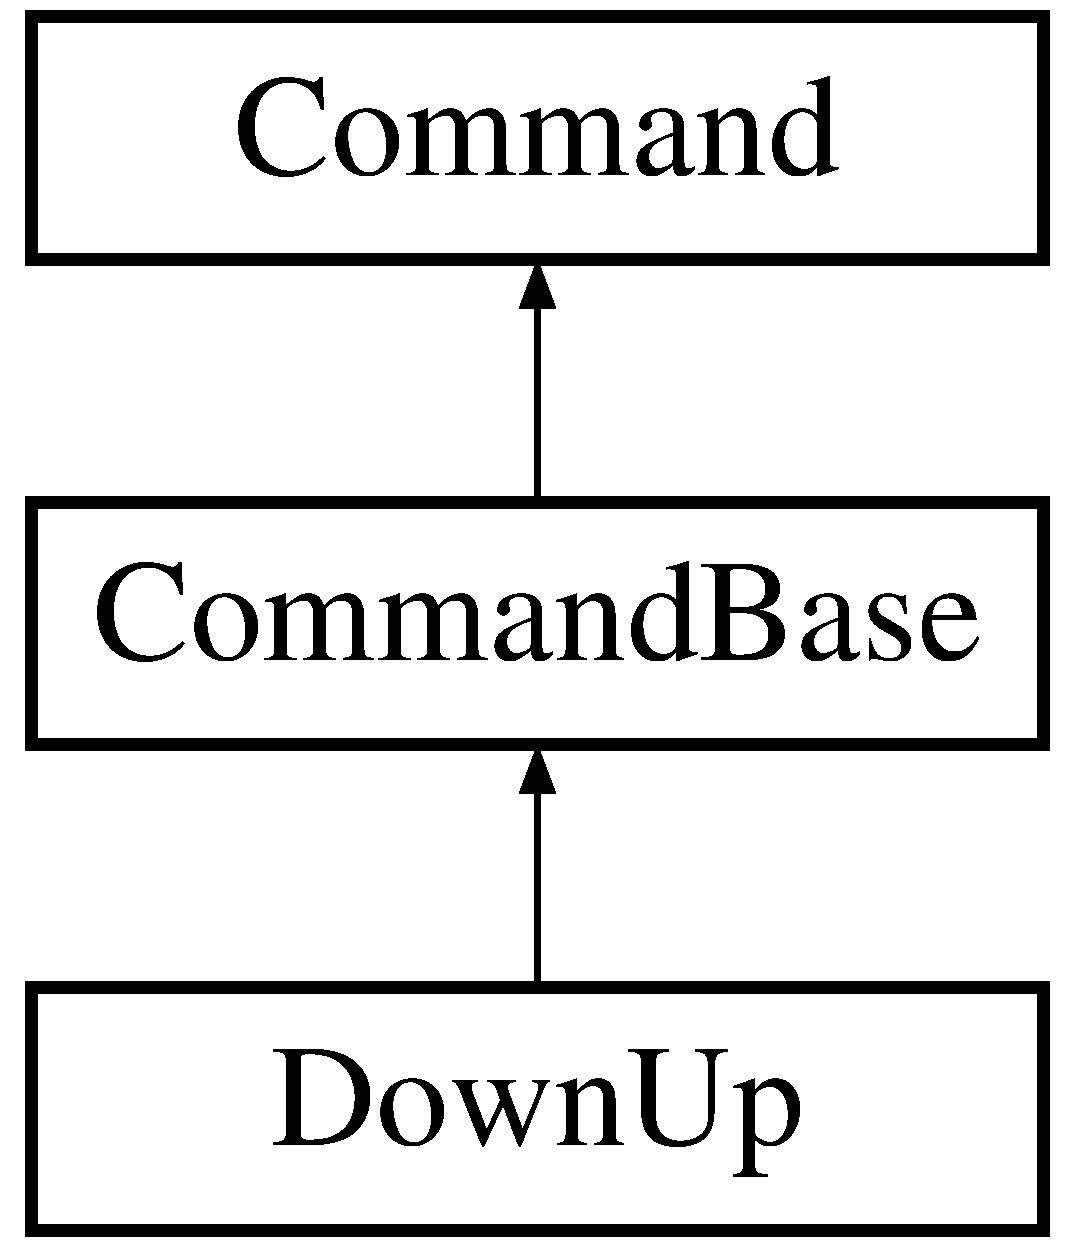
\includegraphics[height=3.000000cm]{class_down_up}
\end{center}
\end{figure}
\subsection*{Public Types}
\begin{DoxyCompactItemize}
\item 
\hypertarget{class_down_up_a97cdf7f274b23a3856fa1f9714fb64a3}{}enum {\bfseries Position} \{ {\bfseries carry}, 
{\bfseries load}
 \}\label{class_down_up_a97cdf7f274b23a3856fa1f9714fb64a3}

\end{DoxyCompactItemize}
\subsection*{Public Member Functions}
\begin{DoxyCompactItemize}
\item 
\hypertarget{class_down_up_a7b54bea97efdec2d132e5c9dc51141fa}{}{\bfseries Down\+Up} (Position pos)\label{class_down_up_a7b54bea97efdec2d132e5c9dc51141fa}

\item 
\hypertarget{class_down_up_ab88d3595bc2e6929505d4d6d292c0f5a}{}void {\bfseries Initialize} ()\label{class_down_up_ab88d3595bc2e6929505d4d6d292c0f5a}

\item 
\hypertarget{class_down_up_ae7908a4df790edf172f0a413793e2dcf}{}void {\bfseries Execute} ()\label{class_down_up_ae7908a4df790edf172f0a413793e2dcf}

\item 
\hypertarget{class_down_up_af1f8ba9675e6238f8ddaa73d29867b05}{}bool {\bfseries Is\+Finished} ()\label{class_down_up_af1f8ba9675e6238f8ddaa73d29867b05}

\item 
\hypertarget{class_down_up_a715d8a538612d3d9291597043e5b7369}{}void {\bfseries End} ()\label{class_down_up_a715d8a538612d3d9291597043e5b7369}

\item 
\hypertarget{class_down_up_a6de6bbf1a16169fed03f6f1566c6c2a4}{}void {\bfseries Interrupted} ()\label{class_down_up_a6de6bbf1a16169fed03f6f1566c6c2a4}

\end{DoxyCompactItemize}
\subsection*{Additional Inherited Members}


The documentation for this class was generated from the following files\+:\begin{DoxyCompactItemize}
\item 
Cyclophosphamide/src/\+Commands/\+Tote\+Lifting/Down\+Up.\+h\item 
Cyclophosphamide/src/\+Commands/\+Tote\+Lifting/Down\+Up.\+cpp\end{DoxyCompactItemize}

\hypertarget{class_drive_bae}{}\section{Drive\+Bae Class Reference}
\label{class_drive_bae}\index{Drive\+Bae@{Drive\+Bae}}


{\ttfamily \#include $<$Drive\+Bae.\+h$>$}

Inheritance diagram for Drive\+Bae\+:\begin{figure}[H]
\begin{center}
\leavevmode
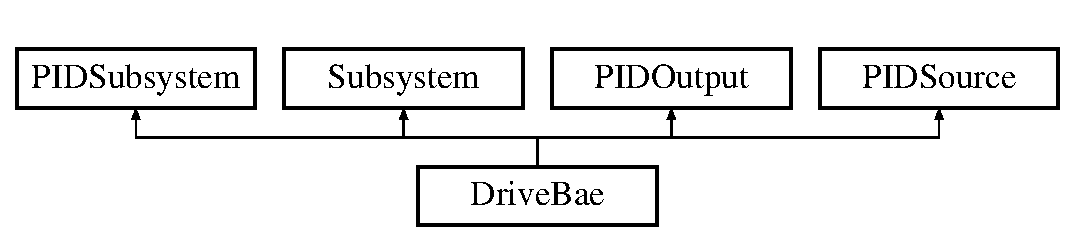
\includegraphics[height=2.000000cm]{class_drive_bae}
\end{center}
\end{figure}
\subsection*{Public Types}
\begin{DoxyCompactItemize}
\item 
\hypertarget{class_drive_bae_a5a16264d8b3e1c0b913d213f194f36a9}{}enum {\bfseries Motor\+Side} \{ {\bfseries F\+R\+O\+N\+T\+\_\+\+L\+E\+F\+T}, 
{\bfseries F\+R\+O\+N\+T\+\_\+\+R\+I\+G\+H\+T}, 
{\bfseries B\+A\+C\+K\+\_\+\+L\+E\+F\+T}, 
{\bfseries B\+A\+C\+K\+\_\+\+R\+I\+G\+H\+T}
 \}\label{class_drive_bae_a5a16264d8b3e1c0b913d213f194f36a9}

\end{DoxyCompactItemize}
\subsection*{Public Member Functions}
\begin{DoxyCompactItemize}
\item 
\hypertarget{class_drive_bae_acaf84db82e4cf983a7af983e39f81b45}{}void {\bfseries enable\+Strafe\+P\+I\+D} (bool state)\label{class_drive_bae_acaf84db82e4cf983a7af983e39f81b45}

\item 
\hypertarget{class_drive_bae_aadff4067d0f5558bd5678f8e52dffb32}{}void {\bfseries set\+Strafe\+Set\+Point} (double set\+Point)\label{class_drive_bae_aadff4067d0f5558bd5678f8e52dffb32}

\item 
\hypertarget{class_drive_bae_ac2497d0afa36b5c72f2ee86f8fd892cf}{}double {\bfseries Return\+P\+I\+D\+Input} ()\label{class_drive_bae_ac2497d0afa36b5c72f2ee86f8fd892cf}

\item 
\hypertarget{class_drive_bae_a423ddc49659be37aed2c0509cc55289b}{}void {\bfseries Use\+P\+I\+D\+Output} (double output)\label{class_drive_bae_a423ddc49659be37aed2c0509cc55289b}

\item 
\hypertarget{class_drive_bae_a2adbbdb59bb0fdc9ed466a3d2edd92ff}{}void {\bfseries Init\+Default\+Command} ()\label{class_drive_bae_a2adbbdb59bb0fdc9ed466a3d2edd92ff}

\item 
\hypertarget{class_drive_bae_a1d381de7dfb03bd3dd138a889c01e880}{}void {\bfseries set\+Speed} (double speed\+Front\+Left, double speed\+Front\+Right, double speed\+Back\+Left, double speed\+Back\+Right)\label{class_drive_bae_a1d381de7dfb03bd3dd138a889c01e880}

\item 
\hypertarget{class_drive_bae_ae0cfe1125d3065eb915111e29e49281c}{}\hyperlink{class_i_m_u}{I\+M\+U} $\ast$ {\bfseries get\+Gyro} ()\label{class_drive_bae_ae0cfe1125d3065eb915111e29e49281c}

\item 
\hypertarget{class_drive_bae_a489a12b403e0b818083402007ea2e314}{}void {\bfseries set\+Target\+Angle} (double theta)\label{class_drive_bae_a489a12b403e0b818083402007ea2e314}

\item 
\hypertarget{class_drive_bae_ab6042ad688723f278787c3747de2f263}{}void {\bfseries stop\+Rot\+P\+I\+D} ()\label{class_drive_bae_ab6042ad688723f278787c3747de2f263}

\item 
\hypertarget{class_drive_bae_aad5e482e88ca3b39ca054cea1217dc6b}{}void {\bfseries start\+Rot\+P\+I\+D} ()\label{class_drive_bae_aad5e482e88ca3b39ca054cea1217dc6b}

\item 
\hypertarget{class_drive_bae_a813f9dfbe7bf7691de735c74e88548d2}{}double {\bfseries get\+Error} ()\label{class_drive_bae_a813f9dfbe7bf7691de735c74e88548d2}

\item 
\hypertarget{class_drive_bae_aaf5602f89bd043412f984251d458e74e}{}double {\bfseries get\+Setpoint} ()\label{class_drive_bae_aaf5602f89bd043412f984251d458e74e}

\item 
\hypertarget{class_drive_bae_a1b22dfabc63aa778c4a5d7eeef1c02e1}{}void {\bfseries set\+Setpoint} (float f)\label{class_drive_bae_a1b22dfabc63aa778c4a5d7eeef1c02e1}

\item 
\hypertarget{class_drive_bae_af8fc09ba2643e2813f46435592b86b3a}{}void {\bfseries set\+Gyro\+Enabled} (bool enable)\label{class_drive_bae_af8fc09ba2643e2813f46435592b86b3a}

\item 
\hypertarget{class_drive_bae_aa43736f6a503bac3f7bfb968a318e831}{}bool {\bfseries is\+Gyro\+Enabled} ()\label{class_drive_bae_aa43736f6a503bac3f7bfb968a318e831}

\item 
\hypertarget{class_drive_bae_a4b480bb19d803cffa8bac5fc3693bc1d}{}void {\bfseries zero\+P\+I\+D\+Output} ()\label{class_drive_bae_a4b480bb19d803cffa8bac5fc3693bc1d}

\item 
\hypertarget{class_drive_bae_a9e669140b1e6f1bd467a89df6fa1fed4}{}void {\bfseries set\+P\+I\+D\+All} (double P, double I, double D)\label{class_drive_bae_a9e669140b1e6f1bd467a89df6fa1fed4}

\item 
\hypertarget{class_drive_bae_abe2f4a4de059ac1479a165a07994a33c}{}void {\bfseries set\+All} (double set\+Point)\label{class_drive_bae_abe2f4a4de059ac1479a165a07994a33c}

\item 
\hypertarget{class_drive_bae_a210429543400fa3789576b1591ec4179}{}void {\bfseries enable\+P\+I\+D\+All} (bool state)\label{class_drive_bae_a210429543400fa3789576b1591ec4179}

\item 
\hypertarget{class_drive_bae_a7b6936f81aa8249e36998f3e371d44d9}{}void {\bfseries set\+Mode\+All} (C\+A\+N\+Talon\+::\+Control\+Mode mode)\label{class_drive_bae_a7b6936f81aa8249e36998f3e371d44d9}

\item 
\hypertarget{class_drive_bae_a332eee2604b94a0a79af935242d7e260}{}void {\bfseries zero\+Encoders} ()\label{class_drive_bae_a332eee2604b94a0a79af935242d7e260}

\item 
\hypertarget{class_drive_bae_a547909d641c7a890c427b154f982322d}{}bool {\bfseries within\+Threshhold} (double drive\+Threshhold, double target\+Distance)\label{class_drive_bae_a547909d641c7a890c427b154f982322d}

\item 
\hypertarget{class_drive_bae_ab09e8a797848efa2a1f2eb6844941cb3}{}void {\bfseries set\+Forward} (double f)\label{class_drive_bae_ab09e8a797848efa2a1f2eb6844941cb3}

\item 
\hypertarget{class_drive_bae_a4fcdfa68a38e020a0497f6256989fe0b}{}void {\bfseries set\+Right} (double r)\label{class_drive_bae_a4fcdfa68a38e020a0497f6256989fe0b}

\item 
\hypertarget{class_drive_bae_a088352135fb6a558c93c0c9da74e37e2}{}void {\bfseries set\+Clockwise} (double c)\label{class_drive_bae_a088352135fb6a558c93c0c9da74e37e2}

\item 
\hypertarget{class_drive_bae_a361b5a623c8e04643a5545daa795876b}{}double {\bfseries get\+Forward} ()\label{class_drive_bae_a361b5a623c8e04643a5545daa795876b}

\item 
\hypertarget{class_drive_bae_ac7fac12731fced5d6e9a7289fb9be485}{}double {\bfseries get\+Clockwise} ()\label{class_drive_bae_ac7fac12731fced5d6e9a7289fb9be485}

\item 
\hypertarget{class_drive_bae_a8b51a78cedeb43380363361e490fa5b5}{}double {\bfseries get\+Right} ()\label{class_drive_bae_a8b51a78cedeb43380363361e490fa5b5}

\item 
\hypertarget{class_drive_bae_aa64c38e02e64ee7795f4ae06bab26d48}{}void {\bfseries execute} ()\label{class_drive_bae_aa64c38e02e64ee7795f4ae06bab26d48}

\item 
\hypertarget{class_drive_bae_aec401bb78b3961da28c0fb36b2308ca4}{}virtual void {\bfseries P\+I\+D\+Write} (float f)\label{class_drive_bae_aec401bb78b3961da28c0fb36b2308ca4}

\item 
\hypertarget{class_drive_bae_ac4a719afe5c71f716c8753392ae0c6fd}{}virtual double {\bfseries P\+I\+D\+Get} ()\label{class_drive_bae_ac4a719afe5c71f716c8753392ae0c6fd}

\item 
\hypertarget{class_drive_bae_a06177effa3aedbcf3874701a93f36f9c}{}D\+R\+I\+V\+E\+\_\+\+M\+O\+T\+O\+R\+\_\+\+T\+Y\+P\+E $\ast$ {\bfseries get\+Motor} (Motor\+Side side)\label{class_drive_bae_a06177effa3aedbcf3874701a93f36f9c}

\end{DoxyCompactItemize}


\subsection{Detailed Description}
The \hyperlink{class_drive_bae}{Drive\+Bae} drives with field centric. 

The documentation for this class was generated from the following files\+:\begin{DoxyCompactItemize}
\item 
Cyclophosphamide/src/\+Subsystems/Drive\+Bae.\+h\item 
Cyclophosphamide/src/\+Subsystems/Drive\+Bae.\+cpp\end{DoxyCompactItemize}

\hypertarget{class_i_m_u}{}\section{I\+M\+U Class Reference}
\label{class_i_m_u}\index{I\+M\+U@{I\+M\+U}}
Inheritance diagram for I\+M\+U\+:\begin{figure}[H]
\begin{center}
\leavevmode
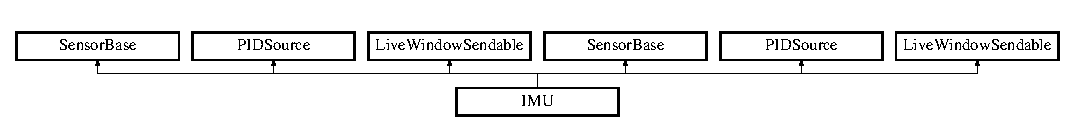
\includegraphics[height=2.000000cm]{class_i_m_u}
\end{center}
\end{figure}
\subsection*{Public Member Functions}
\begin{DoxyCompactItemize}
\item 
\hypertarget{class_i_m_u_ae843cd598703cc3a38e8839aa3371c81}{}{\bfseries I\+M\+U} (Serial\+Port $\ast$pport, uint8\+\_\+t update\+\_\+rate\+\_\+hz=100)\label{class_i_m_u_ae843cd598703cc3a38e8839aa3371c81}

\item 
virtual \hyperlink{class_i_m_u_ad1f213d1e6aa08988ff683feab721559}{$\sim$\+I\+M\+U} ()
\item 
\hypertarget{class_i_m_u_ad5609b0448030d3eec8f59ad83b6291d}{}virtual float {\bfseries Get\+Pitch} ()\label{class_i_m_u_ad5609b0448030d3eec8f59ad83b6291d}

\item 
\hypertarget{class_i_m_u_adcd153b775a8d219d9256ca6390b2003}{}virtual float {\bfseries Get\+Roll} ()\label{class_i_m_u_adcd153b775a8d219d9256ca6390b2003}

\item 
virtual float \hyperlink{class_i_m_u_aecfad6302ad01869e1959b1d27fc4df1}{Get\+Yaw} ()
\item 
\hypertarget{class_i_m_u_af5503d6c0702237197c5308b250c6a39}{}virtual float {\bfseries Get\+Compass\+Heading} ()\label{class_i_m_u_af5503d6c0702237197c5308b250c6a39}

\item 
\hypertarget{class_i_m_u_a9d0d770cb38985e5c3ab35d1cd09b3e2}{}bool {\bfseries Is\+Connected} ()\label{class_i_m_u_a9d0d770cb38985e5c3ab35d1cd09b3e2}

\item 
\hypertarget{class_i_m_u_acb3fa9e821ed200dd7f39cd4ae94b7c1}{}void {\bfseries Zero\+Yaw} ()\label{class_i_m_u_acb3fa9e821ed200dd7f39cd4ae94b7c1}

\item 
double \hyperlink{class_i_m_u_a8484485e99ecdd6647059c307344f82d}{P\+I\+D\+Get} ()
\item 
\hypertarget{class_i_m_u_ab0dbda1a844ff67053b079b0dc9cb2d2}{}void {\bfseries Update\+Table} ()\label{class_i_m_u_ab0dbda1a844ff67053b079b0dc9cb2d2}

\item 
\hypertarget{class_i_m_u_aeb6fa87e7c59b22468102cb880948f8c}{}void {\bfseries Start\+Live\+Window\+Mode} ()\label{class_i_m_u_aeb6fa87e7c59b22468102cb880948f8c}

\item 
\hypertarget{class_i_m_u_ad84477436f7a01306204f74a917428fa}{}void {\bfseries Stop\+Live\+Window\+Mode} ()\label{class_i_m_u_ad84477436f7a01306204f74a917428fa}

\item 
\hypertarget{class_i_m_u_ac1b122983651c9f0d8892aceecaaba7e}{}std\+::string {\bfseries Get\+Smart\+Dashboard\+Type} ()\label{class_i_m_u_ac1b122983651c9f0d8892aceecaaba7e}

\item 
\hypertarget{class_i_m_u_a0f1e2ba7829c650d1e423f51db79fab0}{}void {\bfseries Init\+Table} (I\+Table $\ast$sub\+Table)\label{class_i_m_u_a0f1e2ba7829c650d1e423f51db79fab0}

\item 
\hypertarget{class_i_m_u_a46fafeeb45fa63fd8876501fb270eaa9}{}I\+Table $\ast$ {\bfseries Get\+Table} ()\label{class_i_m_u_a46fafeeb45fa63fd8876501fb270eaa9}

\item 
\hypertarget{class_i_m_u_ad9b522b7a9e8843d1d042f22accb3d03}{}Serial\+Port $\ast$ {\bfseries Get\+Serial\+Port} ()\label{class_i_m_u_ad9b522b7a9e8843d1d042f22accb3d03}

\item 
\hypertarget{class_i_m_u_aa1e9bc2d755f8ec367d13b7440554a9c}{}void {\bfseries Set\+Yaw\+Pitch\+Roll} (float yaw, float pitch, float roll, float compass\+\_\+heading)\label{class_i_m_u_aa1e9bc2d755f8ec367d13b7440554a9c}

\item 
\hypertarget{class_i_m_u_a3c355546b9b43fa8fb5d82d5dd030ca1}{}void {\bfseries Set\+Stream\+Response} (char stream\+\_\+type, uint16\+\_\+t gyro\+\_\+fsr\+\_\+dps, uint16\+\_\+t accel\+\_\+fsr\+\_\+g, uint16\+\_\+t update\+\_\+rate\+\_\+hz, float yaw\+\_\+offset\+\_\+degrees, uint16\+\_\+t q1\+\_\+offset, uint16\+\_\+t q2\+\_\+offset, uint16\+\_\+t q3\+\_\+offset, uint16\+\_\+t q4\+\_\+offset, uint16\+\_\+t flags)\label{class_i_m_u_a3c355546b9b43fa8fb5d82d5dd030ca1}

\item 
\hypertarget{class_i_m_u_abff8d4585010a9d47ac436a3b88c75a4}{}double {\bfseries Get\+Yaw\+Offset} ()\label{class_i_m_u_abff8d4585010a9d47ac436a3b88c75a4}

\item 
\hypertarget{class_i_m_u_a35cf0cb6759d187a1d436865aeda8720}{}double {\bfseries Get\+Byte\+Count} ()\label{class_i_m_u_a35cf0cb6759d187a1d436865aeda8720}

\item 
\hypertarget{class_i_m_u_aeaa93015313fcc79326bb5e81ab48e00}{}double {\bfseries Get\+Update\+Count} ()\label{class_i_m_u_aeaa93015313fcc79326bb5e81ab48e00}

\item 
\hypertarget{class_i_m_u_acc57c44ede00d36ece51325dcd2f9b1e}{}void {\bfseries Restart} ()\label{class_i_m_u_acc57c44ede00d36ece51325dcd2f9b1e}

\item 
\hypertarget{class_i_m_u_a487c9c4355277cebe1a3b4bcc05b58d1}{}bool {\bfseries Is\+Calibrating} ()\label{class_i_m_u_a487c9c4355277cebe1a3b4bcc05b58d1}

\item 
\hypertarget{class_i_m_u_ab7cc1a50aa8aafa63662a87086ef5282}{}virtual int {\bfseries Decode\+Packet\+Handler} (char $\ast$received\+\_\+data, int bytes\+\_\+remaining)\label{class_i_m_u_ab7cc1a50aa8aafa63662a87086ef5282}

\end{DoxyCompactItemize}
\subsection*{Public Attributes}
\begin{DoxyCompactItemize}
\item 
\hypertarget{class_i_m_u_a31e9059f2a805339c1ef3fb210276f2d}{}uint8\+\_\+t {\bfseries update\+\_\+rate\+\_\+hz}\label{class_i_m_u_a31e9059f2a805339c1ef3fb210276f2d}

\item 
\hypertarget{class_i_m_u_af8556bf9f3d975571e340656388bbc6c}{}char {\bfseries current\+\_\+stream\+\_\+type}\label{class_i_m_u_af8556bf9f3d975571e340656388bbc6c}

\end{DoxyCompactItemize}
\subsection*{Protected Member Functions}
\begin{DoxyCompactItemize}
\item 
\hypertarget{class_i_m_u_a5768eb5fa968177300dd9e4a16bda86f}{}{\bfseries I\+M\+U} (Serial\+Port $\ast$pport, uint8\+\_\+t update\+\_\+rate\+\_\+hz, char stream\+\_\+type)\label{class_i_m_u_a5768eb5fa968177300dd9e4a16bda86f}

\item 
\hypertarget{class_i_m_u_a8032d6903cf70281086c07ebdfe16b80}{}void {\bfseries Internal\+Init} (Serial\+Port $\ast$pport, uint8\+\_\+t update\+\_\+rate\+\_\+hz, char stream\+\_\+type)\label{class_i_m_u_a8032d6903cf70281086c07ebdfe16b80}

\item 
\hypertarget{class_i_m_u_ad005f8d336dbfc0fd53efdb8c3976fc9}{}void {\bfseries Update\+Yaw\+History} (float curr\+\_\+yaw)\label{class_i_m_u_ad005f8d336dbfc0fd53efdb8c3976fc9}

\end{DoxyCompactItemize}
\subsection*{Protected Attributes}
\begin{DoxyCompactItemize}
\item 
\hypertarget{class_i_m_u_a3051ad2cef2cd87af8da5b9d84ec4617}{}Serial\+Port $\ast$ {\bfseries pserial\+\_\+port}\label{class_i_m_u_a3051ad2cef2cd87af8da5b9d84ec4617}

\item 
\hypertarget{class_i_m_u_ae3b704880e2a11a2e6b4e39737b6cd20}{}Task $\ast$ {\bfseries m\+\_\+task}\label{class_i_m_u_ae3b704880e2a11a2e6b4e39737b6cd20}

\item 
\hypertarget{class_i_m_u_abafcc13ad5e5bbe902188b5d15b83240}{}float {\bfseries yaw}\label{class_i_m_u_abafcc13ad5e5bbe902188b5d15b83240}

\item 
\hypertarget{class_i_m_u_afbeac482b873f4eabfc8f85009ce2c42}{}float {\bfseries pitch}\label{class_i_m_u_afbeac482b873f4eabfc8f85009ce2c42}

\item 
\hypertarget{class_i_m_u_acd6447159ca43d07412eedd0ae1ace58}{}float {\bfseries roll}\label{class_i_m_u_acd6447159ca43d07412eedd0ae1ace58}

\item 
\hypertarget{class_i_m_u_ab2505b0243397689c271de042a913536}{}float {\bfseries compass\+\_\+heading}\label{class_i_m_u_ab2505b0243397689c271de042a913536}

\item 
\hypertarget{class_i_m_u_a4cb351f7a90d95a399c83e23f916fbb6}{}float {\bfseries yaw\+\_\+history} \mbox{[}Y\+A\+W\+\_\+\+H\+I\+S\+T\+O\+R\+Y\+\_\+\+L\+E\+N\+G\+T\+H\mbox{]}\label{class_i_m_u_a4cb351f7a90d95a399c83e23f916fbb6}

\item 
\hypertarget{class_i_m_u_a39770f45709b018ab4caa1c7c7b950d9}{}int {\bfseries next\+\_\+yaw\+\_\+history\+\_\+index}\label{class_i_m_u_a39770f45709b018ab4caa1c7c7b950d9}

\item 
\hypertarget{class_i_m_u_af6e9bbef741b76157a0d7c4db722f525}{}double {\bfseries last\+\_\+update\+\_\+time}\label{class_i_m_u_af6e9bbef741b76157a0d7c4db722f525}

\item 
\hypertarget{class_i_m_u_aeed5a2a480ebd5dcad81192c39712ef4}{}double {\bfseries yaw\+\_\+offset}\label{class_i_m_u_aeed5a2a480ebd5dcad81192c39712ef4}

\item 
\hypertarget{class_i_m_u_a0ef11d2a7d46e164daeba17fc8b92920}{}float {\bfseries yaw\+\_\+offset\+\_\+degrees}\label{class_i_m_u_a0ef11d2a7d46e164daeba17fc8b92920}

\item 
\hypertarget{class_i_m_u_a000deee3d33d1b076d431abfc1e6ecd1}{}uint16\+\_\+t {\bfseries accel\+\_\+fsr\+\_\+g}\label{class_i_m_u_a000deee3d33d1b076d431abfc1e6ecd1}

\item 
\hypertarget{class_i_m_u_a08c6d63115ff442a875589f11a6ba864}{}uint16\+\_\+t {\bfseries gyro\+\_\+fsr\+\_\+dps}\label{class_i_m_u_a08c6d63115ff442a875589f11a6ba864}

\item 
\hypertarget{class_i_m_u_a437ced4c5f85c8a246601d47274a92fd}{}uint16\+\_\+t {\bfseries flags}\label{class_i_m_u_a437ced4c5f85c8a246601d47274a92fd}

\item 
\hypertarget{class_i_m_u_a031302356455aa67af956c735bcf91e7}{}I\+Table $\ast$ {\bfseries m\+\_\+table}\label{class_i_m_u_a031302356455aa67af956c735bcf91e7}

\end{DoxyCompactItemize}


\subsection{Constructor \& Destructor Documentation}
\hypertarget{class_i_m_u_ad1f213d1e6aa08988ff683feab721559}{}\index{I\+M\+U@{I\+M\+U}!````~I\+M\+U@{$\sim$\+I\+M\+U}}
\index{````~I\+M\+U@{$\sim$\+I\+M\+U}!I\+M\+U@{I\+M\+U}}
\subsubsection[{$\sim$\+I\+M\+U}]{\setlength{\rightskip}{0pt plus 5cm}I\+M\+U\+::$\sim$\+I\+M\+U (
\begin{DoxyParamCaption}
{}
\end{DoxyParamCaption}
)\hspace{0.3cm}{\ttfamily [virtual]}}\label{class_i_m_u_ad1f213d1e6aa08988ff683feab721559}
Delete the \hyperlink{class_i_m_u}{I\+M\+U}. 

\subsection{Member Function Documentation}
\hypertarget{class_i_m_u_aecfad6302ad01869e1959b1d27fc4df1}{}\index{I\+M\+U@{I\+M\+U}!Get\+Yaw@{Get\+Yaw}}
\index{Get\+Yaw@{Get\+Yaw}!I\+M\+U@{I\+M\+U}}
\subsubsection[{Get\+Yaw}]{\setlength{\rightskip}{0pt plus 5cm}float I\+M\+U\+::\+Get\+Yaw (
\begin{DoxyParamCaption}
\item[{void}]{}
\end{DoxyParamCaption}
)\hspace{0.3cm}{\ttfamily [virtual]}}\label{class_i_m_u_aecfad6302ad01869e1959b1d27fc4df1}
Return the yaw angle in degrees.

This angle increases as the robot spins to the right.

This angle ranges from -\/180 to 180 degrees. \hypertarget{class_i_m_u_a8484485e99ecdd6647059c307344f82d}{}\index{I\+M\+U@{I\+M\+U}!P\+I\+D\+Get@{P\+I\+D\+Get}}
\index{P\+I\+D\+Get@{P\+I\+D\+Get}!I\+M\+U@{I\+M\+U}}
\subsubsection[{P\+I\+D\+Get}]{\setlength{\rightskip}{0pt plus 5cm}double I\+M\+U\+::\+P\+I\+D\+Get (
\begin{DoxyParamCaption}
{}
\end{DoxyParamCaption}
)}\label{class_i_m_u_a8484485e99ecdd6647059c307344f82d}
Get the angle in degrees for the P\+I\+D\+Source base object.

\begin{DoxyReturn}{Returns}
The angle in degrees. 
\end{DoxyReturn}


The documentation for this class was generated from the following files\+:\begin{DoxyCompactItemize}
\item 
Cyclophosphamide/src/\+Gyro\+Driver/I\+M\+U.\+h\item 
Cyclophosphamide/src/\+Gyro\+Driver/I\+M\+U.\+cpp\end{DoxyCompactItemize}

\hypertarget{class_i_m_u_protocol}{}\section{I\+M\+U\+Protocol Class Reference}
\label{class_i_m_u_protocol}\index{I\+M\+U\+Protocol@{I\+M\+U\+Protocol}}
\subsection*{Static Public Member Functions}
\begin{DoxyCompactItemize}
\item 
\hypertarget{class_i_m_u_protocol_a5043b90e784f5810b313489ae45fd19b}{}static int {\bfseries encode\+Y\+P\+R\+Update} (char $\ast$protocol\+\_\+buffer, float yaw, float pitch, float roll, float compass\+\_\+heading)\label{class_i_m_u_protocol_a5043b90e784f5810b313489ae45fd19b}

\item 
\hypertarget{class_i_m_u_protocol_a2076e198a0111d24e7312302529c11fa}{}static int {\bfseries encode\+Quaternion\+Update} (char $\ast$protocol\+\_\+buffer, uint16\+\_\+t q1, uint16\+\_\+t q2, uint16\+\_\+t q3, uint16\+\_\+t q4, uint16\+\_\+t accel\+\_\+x, uint16\+\_\+t accel\+\_\+y, uint16\+\_\+t accel\+\_\+z, int16\+\_\+t mag\+\_\+x, int16\+\_\+t mag\+\_\+y, int16\+\_\+t mag\+\_\+z, float temp\+\_\+c)\label{class_i_m_u_protocol_a2076e198a0111d24e7312302529c11fa}

\item 
\hypertarget{class_i_m_u_protocol_a2ae8e5f0bfe45485ab475335fad6e889}{}static int {\bfseries encode\+Gyro\+Update} (char $\ast$protocol\+\_\+buffer, uint16\+\_\+t gyro\+\_\+x, uint16\+\_\+t gyro\+\_\+y, uint16\+\_\+t gyro\+\_\+z, uint16\+\_\+t accel\+\_\+x, uint16\+\_\+t accel\+\_\+y, uint16\+\_\+t accel\+\_\+z, int16\+\_\+t mag\+\_\+x, int16\+\_\+t mag\+\_\+y, int16\+\_\+t mag\+\_\+z, float temp\+\_\+c)\label{class_i_m_u_protocol_a2ae8e5f0bfe45485ab475335fad6e889}

\item 
\hypertarget{class_i_m_u_protocol_a900c9f6e4174c510765f8885f07bd0e9}{}static int {\bfseries encode\+Stream\+Command} (char $\ast$protocol\+\_\+buffer, char stream\+\_\+type, unsigned char update\+\_\+rate\+\_\+hz)\label{class_i_m_u_protocol_a900c9f6e4174c510765f8885f07bd0e9}

\item 
\hypertarget{class_i_m_u_protocol_a47edf8d27c46da8cb395c14a726a9732}{}static int {\bfseries encode\+Stream\+Response} (char $\ast$protocol\+\_\+buffer, char stream\+\_\+type, uint16\+\_\+t gyro\+\_\+fsr\+\_\+dps, uint16\+\_\+t accel\+\_\+fsr\+\_\+g, uint16\+\_\+t update\+\_\+rate\+\_\+hz, float yaw\+\_\+offset\+\_\+degrees, uint16\+\_\+t q1\+\_\+offset, uint16\+\_\+t q2\+\_\+offset, uint16\+\_\+t q3\+\_\+offset, uint16\+\_\+t q4\+\_\+offset, uint16\+\_\+t flags)\label{class_i_m_u_protocol_a47edf8d27c46da8cb395c14a726a9732}

\item 
\hypertarget{class_i_m_u_protocol_a97c641e18f3881b989a8f89fcb08458c}{}static int {\bfseries decode\+Stream\+Response} (char $\ast$buffer, int length, char \&stream\+\_\+type, uint16\+\_\+t \&gyro\+\_\+fsr\+\_\+dps, uint16\+\_\+t \&accel\+\_\+fsr\+\_\+g, uint16\+\_\+t \&update\+\_\+rate\+\_\+hz, float \&yaw\+\_\+offset\+\_\+degrees, uint16\+\_\+t \&q1\+\_\+offset, uint16\+\_\+t \&q2\+\_\+offset, uint16\+\_\+t \&q3\+\_\+offset, uint16\+\_\+t \&q4\+\_\+offset, uint16\+\_\+t \&flags)\label{class_i_m_u_protocol_a97c641e18f3881b989a8f89fcb08458c}

\item 
\hypertarget{class_i_m_u_protocol_af6c852e5e0fc5fe540d23920e0e2d3a0}{}static int {\bfseries decode\+Stream\+Command} (char $\ast$buffer, int length, char \&stream\+\_\+type, unsigned char \&update\+\_\+rate\+\_\+hz)\label{class_i_m_u_protocol_af6c852e5e0fc5fe540d23920e0e2d3a0}

\item 
\hypertarget{class_i_m_u_protocol_a2a833cb88f11b50e16001e8197ab1664}{}static int {\bfseries decode\+Y\+P\+R\+Update} (char $\ast$buffer, int length, float \&yaw, float \&pitch, float \&roll, float \&compass\+\_\+heading)\label{class_i_m_u_protocol_a2a833cb88f11b50e16001e8197ab1664}

\item 
\hypertarget{class_i_m_u_protocol_a2706f477f4b02197d09d55e436b24fd7}{}static int {\bfseries decode\+Quaternion\+Update} (char $\ast$buffer, int length, int16\+\_\+t \&q1, int16\+\_\+t \&q2, int16\+\_\+t \&q3, int16\+\_\+t \&q4, int16\+\_\+t \&accel\+\_\+x, int16\+\_\+t \&accel\+\_\+y, int16\+\_\+t \&accel\+\_\+z, int16\+\_\+t \&mag\+\_\+x, int16\+\_\+t \&mag\+\_\+y, int16\+\_\+t \&mag\+\_\+z, float \&temp\+\_\+c)\label{class_i_m_u_protocol_a2706f477f4b02197d09d55e436b24fd7}

\item 
\hypertarget{class_i_m_u_protocol_a39d4917878a4af8a173962c1991bbb95}{}static int {\bfseries decode\+Gyro\+Update} (char $\ast$buffer, int length, uint16\+\_\+t \&gyro\+\_\+x, uint16\+\_\+t \&gyro\+\_\+y, uint16\+\_\+t \&gyro\+\_\+z, uint16\+\_\+t \&accel\+\_\+x, uint16\+\_\+t \&accel\+\_\+y, uint16\+\_\+t \&accel\+\_\+z, int16\+\_\+t \&mag\+\_\+x, int16\+\_\+t \&mag\+\_\+y, int16\+\_\+t \&mag\+\_\+z, float \&temp\+\_\+c)\label{class_i_m_u_protocol_a39d4917878a4af8a173962c1991bbb95}

\end{DoxyCompactItemize}
\subsection*{Static Protected Member Functions}
\begin{DoxyCompactItemize}
\item 
\hypertarget{class_i_m_u_protocol_acbe9e784a43ab31c543c772711d0b389}{}static void {\bfseries encode\+Termination} (char $\ast$buffer, int total\+\_\+length, int content\+\_\+length)\label{class_i_m_u_protocol_acbe9e784a43ab31c543c772711d0b389}

\item 
\hypertarget{class_i_m_u_protocol_ad9d78b08dd74af878782c0f4a6c16951}{}static void {\bfseries encode\+Protocol\+Float} (float f, char $\ast$buff)\label{class_i_m_u_protocol_ad9d78b08dd74af878782c0f4a6c16951}

\item 
\hypertarget{class_i_m_u_protocol_af7156807ea5a0488e8eff2beeb1bac40}{}static void {\bfseries encode\+Protocol\+Uint16} (uint16\+\_\+t value, char $\ast$buff)\label{class_i_m_u_protocol_af7156807ea5a0488e8eff2beeb1bac40}

\item 
\hypertarget{class_i_m_u_protocol_a155fa4ff91c441d040988f656094f086}{}static uint16\+\_\+t {\bfseries decode\+Protocol\+Uint16} (char $\ast$uint16\+\_\+string)\label{class_i_m_u_protocol_a155fa4ff91c441d040988f656094f086}

\item 
\hypertarget{class_i_m_u_protocol_ade30772ce94446e5591501a705a22b3f}{}static bool {\bfseries verify\+Checksum} (char $\ast$buffer, int content\+\_\+length)\label{class_i_m_u_protocol_ade30772ce94446e5591501a705a22b3f}

\item 
\hypertarget{class_i_m_u_protocol_a9fae2bd9c887a61936343d7e02d745ed}{}static unsigned char {\bfseries decode\+Uint8} (char $\ast$checksum)\label{class_i_m_u_protocol_a9fae2bd9c887a61936343d7e02d745ed}

\item 
\hypertarget{class_i_m_u_protocol_a91e3d5e6f18c6ebf8499216df493d2f5}{}static float {\bfseries decode\+Protocol\+Float} (char $\ast$buffer)\label{class_i_m_u_protocol_a91e3d5e6f18c6ebf8499216df493d2f5}

\end{DoxyCompactItemize}


The documentation for this class was generated from the following file\+:\begin{DoxyCompactItemize}
\item 
Cyclophosphamide/src/\+Gyro\+Driver/I\+M\+U\+Protocol.\+h\end{DoxyCompactItemize}

\hypertarget{class_induct}{}\section{Induct Class Reference}
\label{class_induct}\index{Induct@{Induct}}


{\ttfamily \#include $<$Induct.\+h$>$}

Inheritance diagram for Induct\+:\begin{figure}[H]
\begin{center}
\leavevmode
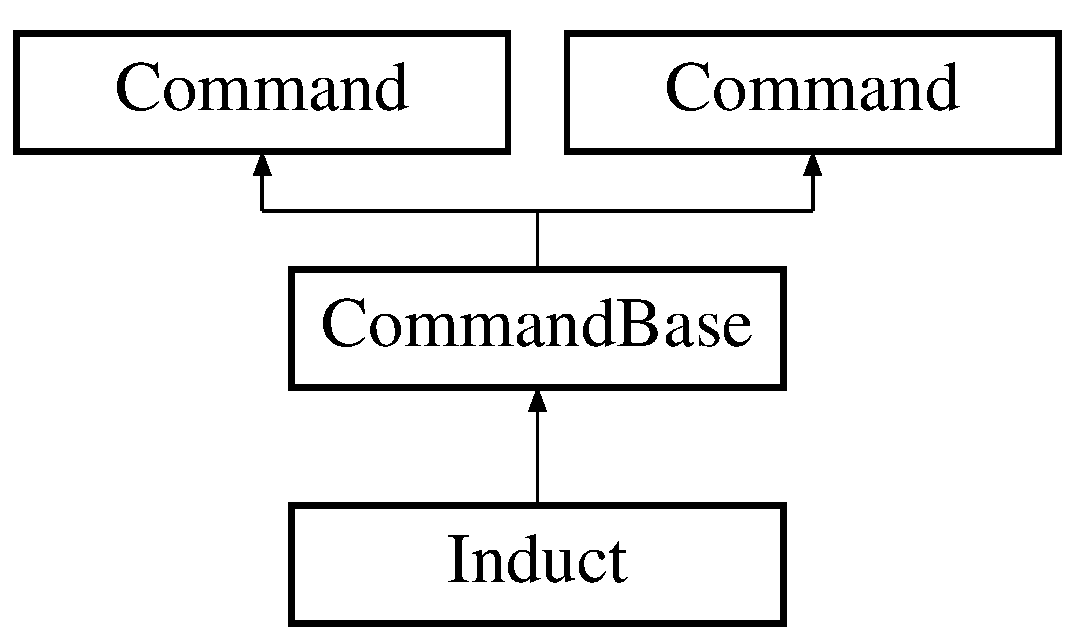
\includegraphics[height=3.000000cm]{class_induct}
\end{center}
\end{figure}
\subsection*{Public Member Functions}
\begin{DoxyCompactItemize}
\item 
\hypertarget{class_induct_a376883b40ea5f30e809258dbc2af25d6}{}void {\bfseries Initialize} ()\label{class_induct_a376883b40ea5f30e809258dbc2af25d6}

\item 
\hypertarget{class_induct_a69b0aab1025a5c5f1913dc9030b608b0}{}void {\bfseries Execute} ()\label{class_induct_a69b0aab1025a5c5f1913dc9030b608b0}

\item 
\hypertarget{class_induct_a23511705e0e9f4fb677bd9790c64d6b6}{}bool {\bfseries Is\+Finished} ()\label{class_induct_a23511705e0e9f4fb677bd9790c64d6b6}

\item 
\hypertarget{class_induct_a2647c17f70beac0ca882cd304d0cd8df}{}void {\bfseries End} ()\label{class_induct_a2647c17f70beac0ca882cd304d0cd8df}

\item 
\hypertarget{class_induct_a4d32fbfac6d16e3ed5f260d9b70001a5}{}void {\bfseries Interrupted} ()\label{class_induct_a4d32fbfac6d16e3ed5f260d9b70001a5}

\end{DoxyCompactItemize}
\subsection*{Additional Inherited Members}


\subsection{Detailed Description}
Sets the motor speed of the can grabbing mecanum motors to zero 

The documentation for this class was generated from the following files\+:\begin{DoxyCompactItemize}
\item 
Cyclophosphamide/src/\+Commands/\+Can\+Collecterino/\+Arms/Induct.\+h\item 
Cyclophosphamide/src/\+Commands/\+Can\+Collecterino/\+Arms/Induct.\+cpp\end{DoxyCompactItemize}

\hypertarget{class_intake_match_drive_base}{}\section{Intake\+Match\+Drive\+Base Class Reference}
\label{class_intake_match_drive_base}\index{Intake\+Match\+Drive\+Base@{Intake\+Match\+Drive\+Base}}
Inheritance diagram for Intake\+Match\+Drive\+Base\+:\begin{figure}[H]
\begin{center}
\leavevmode
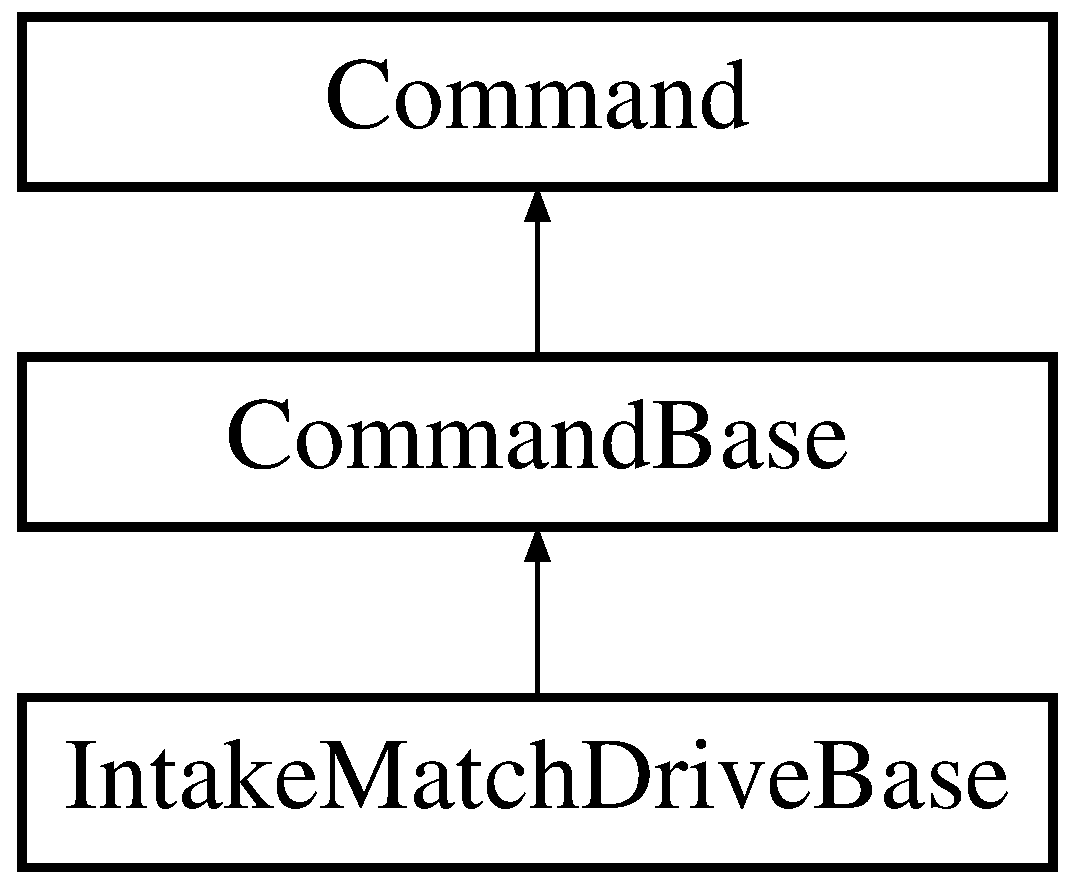
\includegraphics[height=3.000000cm]{class_intake_match_drive_base}
\end{center}
\end{figure}
\subsection*{Public Member Functions}
\begin{DoxyCompactItemize}
\item 
\hypertarget{class_intake_match_drive_base_a6df8780272d10c34a1a013066ee1bb51}{}void {\bfseries Initialize} ()\label{class_intake_match_drive_base_a6df8780272d10c34a1a013066ee1bb51}

\item 
\hypertarget{class_intake_match_drive_base_a7faf75b0dcf853d5c5513be87ae44ee7}{}void {\bfseries Execute} ()\label{class_intake_match_drive_base_a7faf75b0dcf853d5c5513be87ae44ee7}

\item 
\hypertarget{class_intake_match_drive_base_a78228e3ae9123c9c4f02f7f227cae290}{}bool {\bfseries Is\+Finished} ()\label{class_intake_match_drive_base_a78228e3ae9123c9c4f02f7f227cae290}

\item 
\hypertarget{class_intake_match_drive_base_a1a039a7be99a2191de25731134989ab6}{}void {\bfseries End} ()\label{class_intake_match_drive_base_a1a039a7be99a2191de25731134989ab6}

\item 
\hypertarget{class_intake_match_drive_base_a460baf0b948a3a11cc61ac674078e83e}{}void {\bfseries Interrupted} ()\label{class_intake_match_drive_base_a460baf0b948a3a11cc61ac674078e83e}

\end{DoxyCompactItemize}
\subsection*{Additional Inherited Members}


The documentation for this class was generated from the following files\+:\begin{DoxyCompactItemize}
\item 
Cyclophosphamide/src/\+Commands/\+Tote\+Intake/Intake\+Match\+Drive\+Base.\+h\item 
Cyclophosphamide/src/\+Commands/\+Tote\+Intake/Intake\+Match\+Drive\+Base.\+cpp\end{DoxyCompactItemize}

\hypertarget{class_lift_relative}{}\section{Lift\+Relative Class Reference}
\label{class_lift_relative}\index{Lift\+Relative@{Lift\+Relative}}
Inheritance diagram for Lift\+Relative\+:\begin{figure}[H]
\begin{center}
\leavevmode
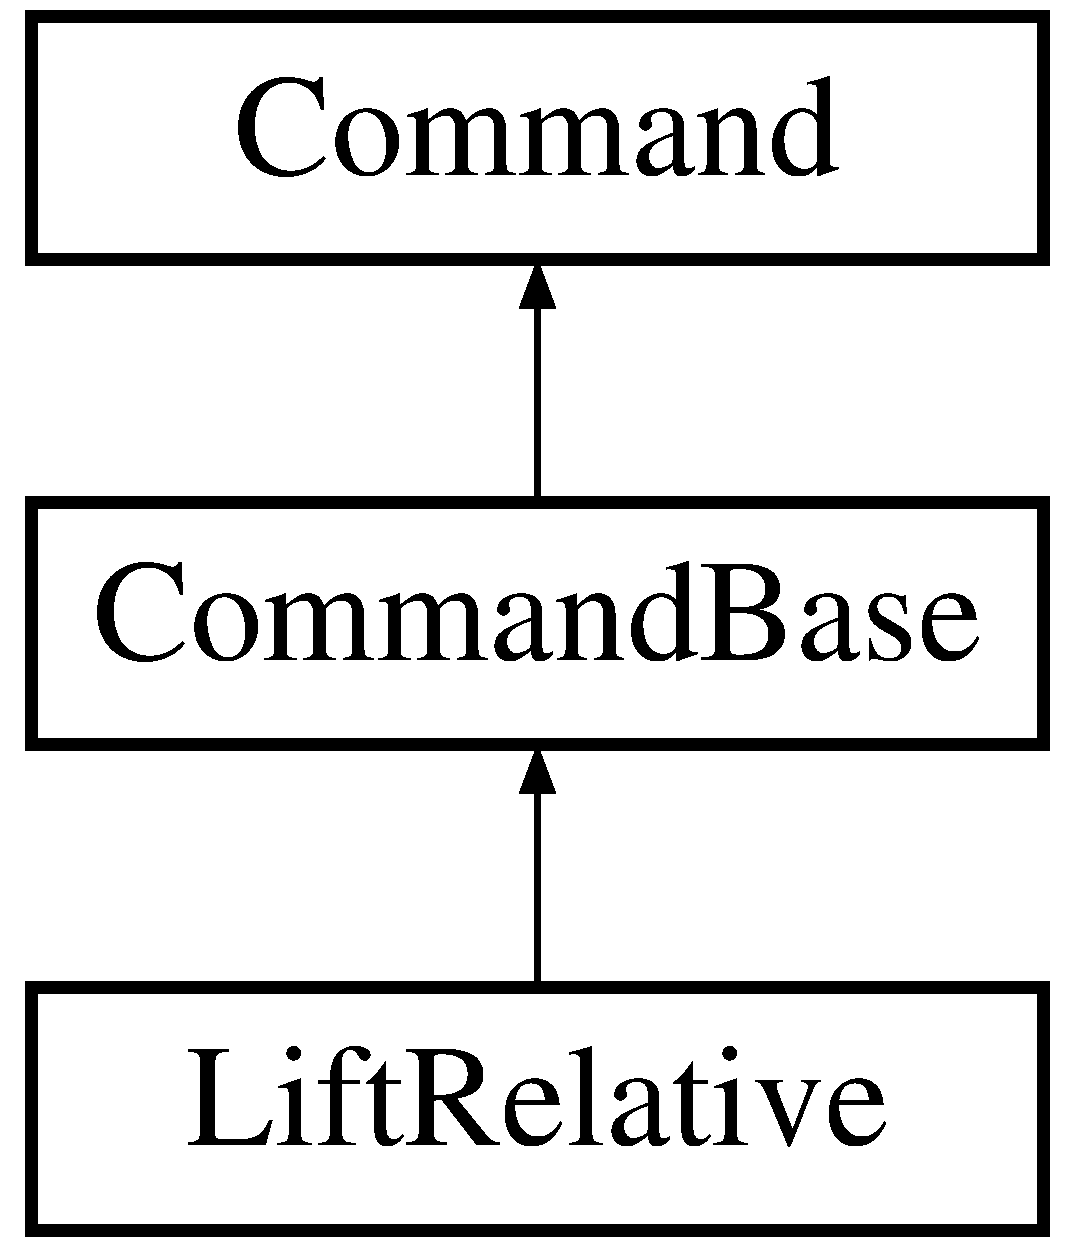
\includegraphics[height=3.000000cm]{class_lift_relative}
\end{center}
\end{figure}
\subsection*{Public Member Functions}
\begin{DoxyCompactItemize}
\item 
\hypertarget{class_lift_relative_a0dd1e44d7e212315d7d305ffd1b7982d}{}{\bfseries Lift\+Relative} (float delta)\label{class_lift_relative_a0dd1e44d7e212315d7d305ffd1b7982d}

\item 
\hypertarget{class_lift_relative_a88ac8dedb8e21a26952bafc5768b6813}{}void {\bfseries Initialize} ()\label{class_lift_relative_a88ac8dedb8e21a26952bafc5768b6813}

\item 
\hypertarget{class_lift_relative_a183fef9c1240a8a78c85d0bd811d6097}{}void {\bfseries Execute} ()\label{class_lift_relative_a183fef9c1240a8a78c85d0bd811d6097}

\item 
\hypertarget{class_lift_relative_a4fdd568331786011beb7522611c3eee0}{}bool {\bfseries Is\+Finished} ()\label{class_lift_relative_a4fdd568331786011beb7522611c3eee0}

\item 
\hypertarget{class_lift_relative_afc4fc4f8e41669406bb14f5b50dda78d}{}void {\bfseries End} ()\label{class_lift_relative_afc4fc4f8e41669406bb14f5b50dda78d}

\item 
\hypertarget{class_lift_relative_a5d2935f2a564a18607d185f3c4d459d1}{}void {\bfseries Interrupted} ()\label{class_lift_relative_a5d2935f2a564a18607d185f3c4d459d1}

\end{DoxyCompactItemize}
\subsection*{Additional Inherited Members}


The documentation for this class was generated from the following files\+:\begin{DoxyCompactItemize}
\item 
Cyclophosphamide/src/\+Commands/\+Tote\+Lifting/Lift\+Relative.\+h\item 
Cyclophosphamide/src/\+Commands/\+Tote\+Lifting/Lift\+Relative.\+cpp\end{DoxyCompactItemize}

\hypertarget{class_lift_to_height}{}\section{Lift\+To\+Height Class Reference}
\label{class_lift_to_height}\index{Lift\+To\+Height@{Lift\+To\+Height}}
Inheritance diagram for Lift\+To\+Height\+:\begin{figure}[H]
\begin{center}
\leavevmode
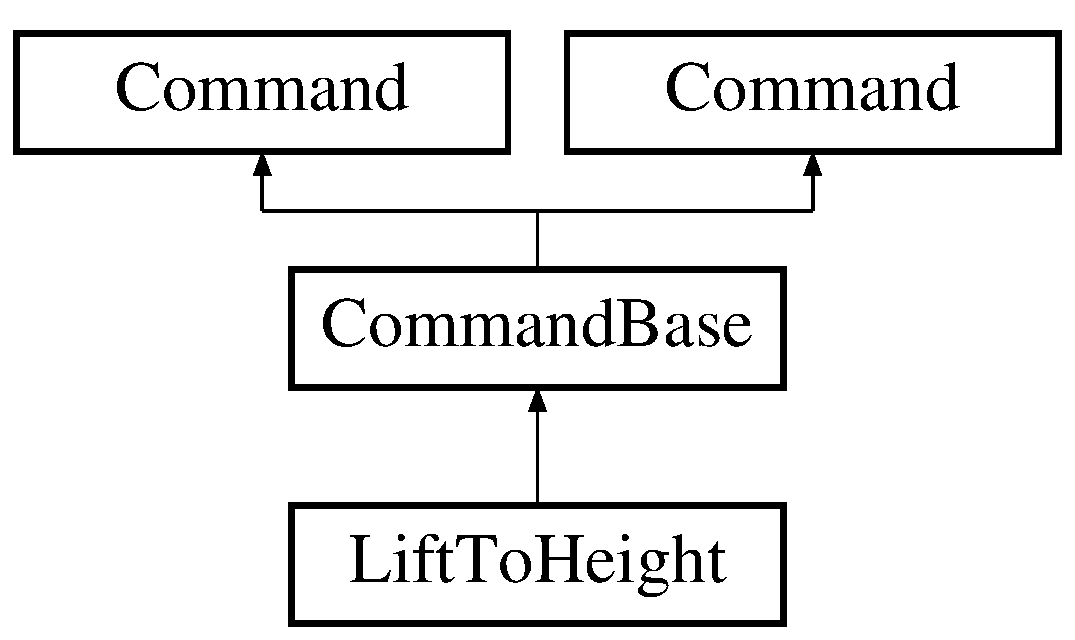
\includegraphics[height=3.000000cm]{class_lift_to_height}
\end{center}
\end{figure}
\subsection*{Public Member Functions}
\begin{DoxyCompactItemize}
\item 
\hypertarget{class_lift_to_height_a01719b438cfc92034741ba204c2ec148}{}{\bfseries Lift\+To\+Height} (double destination)\label{class_lift_to_height_a01719b438cfc92034741ba204c2ec148}

\item 
\hypertarget{class_lift_to_height_a5e78ada1bae3a233eb50d53f0c44adc3}{}void {\bfseries Initialize} ()\label{class_lift_to_height_a5e78ada1bae3a233eb50d53f0c44adc3}

\item 
\hypertarget{class_lift_to_height_a935b281ef6f1bdf0380d9d8df411bd8c}{}void {\bfseries Execute} ()\label{class_lift_to_height_a935b281ef6f1bdf0380d9d8df411bd8c}

\item 
\hypertarget{class_lift_to_height_a0b085aa59453eae9ce4b60271898b1bb}{}bool {\bfseries Is\+Finished} ()\label{class_lift_to_height_a0b085aa59453eae9ce4b60271898b1bb}

\item 
\hypertarget{class_lift_to_height_a1fc76589065de2d7e5df828017fd6e9a}{}void {\bfseries End} ()\label{class_lift_to_height_a1fc76589065de2d7e5df828017fd6e9a}

\item 
\hypertarget{class_lift_to_height_ab967b5415131d8532ee72b23492f7eca}{}void {\bfseries Interrupted} ()\label{class_lift_to_height_ab967b5415131d8532ee72b23492f7eca}

\end{DoxyCompactItemize}
\subsection*{Additional Inherited Members}


The documentation for this class was generated from the following files\+:\begin{DoxyCompactItemize}
\item 
Cyclophosphamide/src/\+Commands/\+Tote\+Handling/Lift\+To\+Height.\+h\item 
Cyclophosphamide/src/\+Commands/\+Tote\+Handling/Lift\+To\+Height.\+cpp\end{DoxyCompactItemize}

\hypertarget{class_lift_to_height_velocity}{}\section{Lift\+To\+Height\+Velocity Class Reference}
\label{class_lift_to_height_velocity}\index{Lift\+To\+Height\+Velocity@{Lift\+To\+Height\+Velocity}}
Inheritance diagram for Lift\+To\+Height\+Velocity\+:\begin{figure}[H]
\begin{center}
\leavevmode
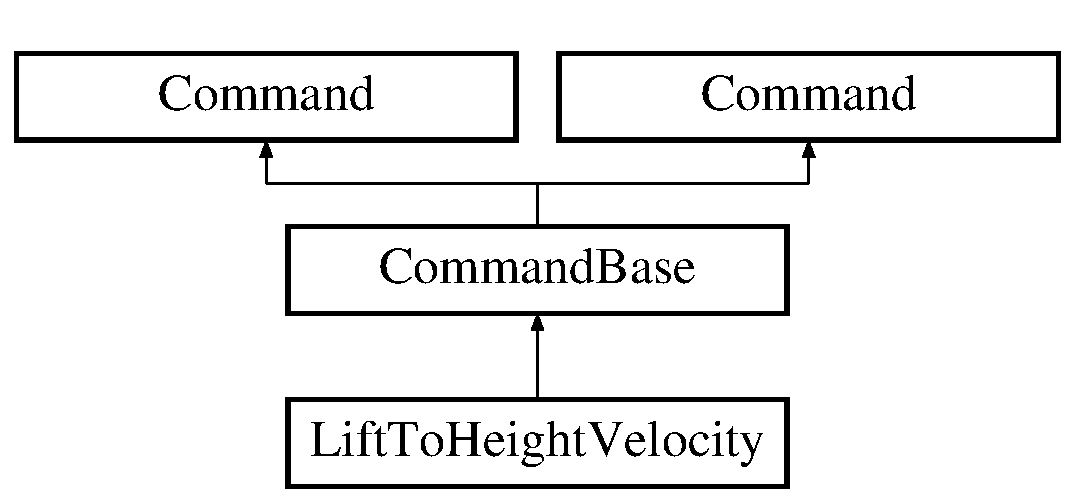
\includegraphics[height=3.000000cm]{class_lift_to_height_velocity}
\end{center}
\end{figure}
\subsection*{Public Member Functions}
\begin{DoxyCompactItemize}
\item 
\hypertarget{class_lift_to_height_velocity_a1c5bf1a887687b2c6a8768df260c983a}{}{\bfseries Lift\+To\+Height\+Velocity} (double speed)\label{class_lift_to_height_velocity_a1c5bf1a887687b2c6a8768df260c983a}

\item 
\hypertarget{class_lift_to_height_velocity_a526c331b5b5fb39f5e96ac3ebfb7202f}{}void {\bfseries Initialize} ()\label{class_lift_to_height_velocity_a526c331b5b5fb39f5e96ac3ebfb7202f}

\item 
\hypertarget{class_lift_to_height_velocity_a751bc1d502d16a64f02dae0aef53dda9}{}void {\bfseries Execute} ()\label{class_lift_to_height_velocity_a751bc1d502d16a64f02dae0aef53dda9}

\item 
\hypertarget{class_lift_to_height_velocity_a9306a5fa5331d2568e78f480d530f09d}{}bool {\bfseries Is\+Finished} ()\label{class_lift_to_height_velocity_a9306a5fa5331d2568e78f480d530f09d}

\item 
\hypertarget{class_lift_to_height_velocity_afb3af180b244bbc9cd49c3ac64fa9fcd}{}void {\bfseries End} ()\label{class_lift_to_height_velocity_afb3af180b244bbc9cd49c3ac64fa9fcd}

\item 
\hypertarget{class_lift_to_height_velocity_a17d8e48fb04b90e777c5e0325ac73f5f}{}void {\bfseries Interrupted} ()\label{class_lift_to_height_velocity_a17d8e48fb04b90e777c5e0325ac73f5f}

\end{DoxyCompactItemize}
\subsection*{Additional Inherited Members}


The documentation for this class was generated from the following files\+:\begin{DoxyCompactItemize}
\item 
Cyclophosphamide/src/\+Commands/\+Tote\+Handling/Lift\+To\+Height\+Velocity.\+h\item 
Cyclophosphamide/src/\+Commands/\+Tote\+Handling/Lift\+To\+Height\+Velocity.\+cpp\end{DoxyCompactItemize}

\hypertarget{class_mecanum_drive}{}\section{Mecanum\+Drive Class Reference}
\label{class_mecanum_drive}\index{Mecanum\+Drive@{Mecanum\+Drive}}
Inheritance diagram for Mecanum\+Drive\+:\begin{figure}[H]
\begin{center}
\leavevmode
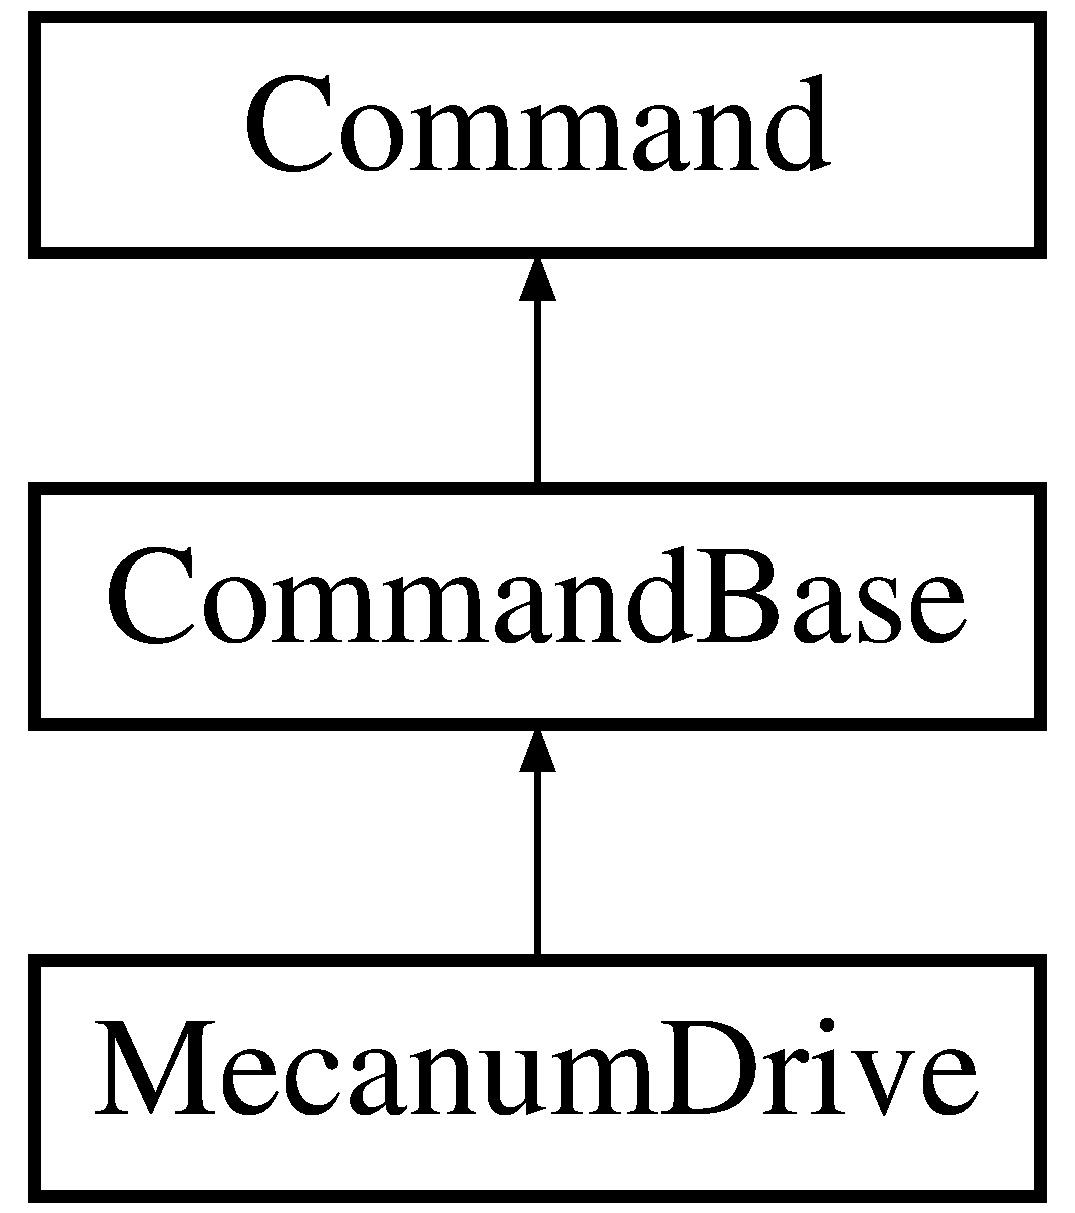
\includegraphics[height=3.000000cm]{class_mecanum_drive}
\end{center}
\end{figure}
\subsection*{Public Member Functions}
\begin{DoxyCompactItemize}
\item 
\hypertarget{class_mecanum_drive_a3bb39fbfc65c1ab74bcb89cee858d324}{}void {\bfseries Initialize} ()\label{class_mecanum_drive_a3bb39fbfc65c1ab74bcb89cee858d324}

\item 
\hypertarget{class_mecanum_drive_aa36e8c7458c2187dbe0a9996c9faf71a}{}void {\bfseries Execute} ()\label{class_mecanum_drive_aa36e8c7458c2187dbe0a9996c9faf71a}

\item 
\hypertarget{class_mecanum_drive_a0da7dc004a592c49fe09eb4fc0e5cb26}{}bool {\bfseries Is\+Finished} ()\label{class_mecanum_drive_a0da7dc004a592c49fe09eb4fc0e5cb26}

\item 
\hypertarget{class_mecanum_drive_a50daee6870028ab2ec3f32ef4b3328be}{}void {\bfseries End} ()\label{class_mecanum_drive_a50daee6870028ab2ec3f32ef4b3328be}

\item 
\hypertarget{class_mecanum_drive_a2739d27b3ac9936bdd9277a9eddb6bd1}{}void {\bfseries Interrupted} ()\label{class_mecanum_drive_a2739d27b3ac9936bdd9277a9eddb6bd1}

\item 
\hypertarget{class_mecanum_drive_a3bb39fbfc65c1ab74bcb89cee858d324}{}void {\bfseries Initialize} ()\label{class_mecanum_drive_a3bb39fbfc65c1ab74bcb89cee858d324}

\item 
\hypertarget{class_mecanum_drive_aa36e8c7458c2187dbe0a9996c9faf71a}{}void {\bfseries Execute} ()\label{class_mecanum_drive_aa36e8c7458c2187dbe0a9996c9faf71a}

\item 
\hypertarget{class_mecanum_drive_a0da7dc004a592c49fe09eb4fc0e5cb26}{}bool {\bfseries Is\+Finished} ()\label{class_mecanum_drive_a0da7dc004a592c49fe09eb4fc0e5cb26}

\item 
\hypertarget{class_mecanum_drive_a50daee6870028ab2ec3f32ef4b3328be}{}void {\bfseries End} ()\label{class_mecanum_drive_a50daee6870028ab2ec3f32ef4b3328be}

\item 
\hypertarget{class_mecanum_drive_a2739d27b3ac9936bdd9277a9eddb6bd1}{}void {\bfseries Interrupted} ()\label{class_mecanum_drive_a2739d27b3ac9936bdd9277a9eddb6bd1}

\end{DoxyCompactItemize}
\subsection*{Additional Inherited Members}


The documentation for this class was generated from the following files\+:\begin{DoxyCompactItemize}
\item 
Cyclophosphamide/src/\+Commands/\+Drivebase/Mecanum\+Drive.\+h\item 
Cyclophosphamide/src/\+Commands/\+Drivebase/Mecanum\+Drive.\+cpp\end{DoxyCompactItemize}

\hypertarget{class_move_arms_fancy}{}\section{Move\+Arms\+Fancy Class Reference}
\label{class_move_arms_fancy}\index{Move\+Arms\+Fancy@{Move\+Arms\+Fancy}}
Inheritance diagram for Move\+Arms\+Fancy\+:\begin{figure}[H]
\begin{center}
\leavevmode
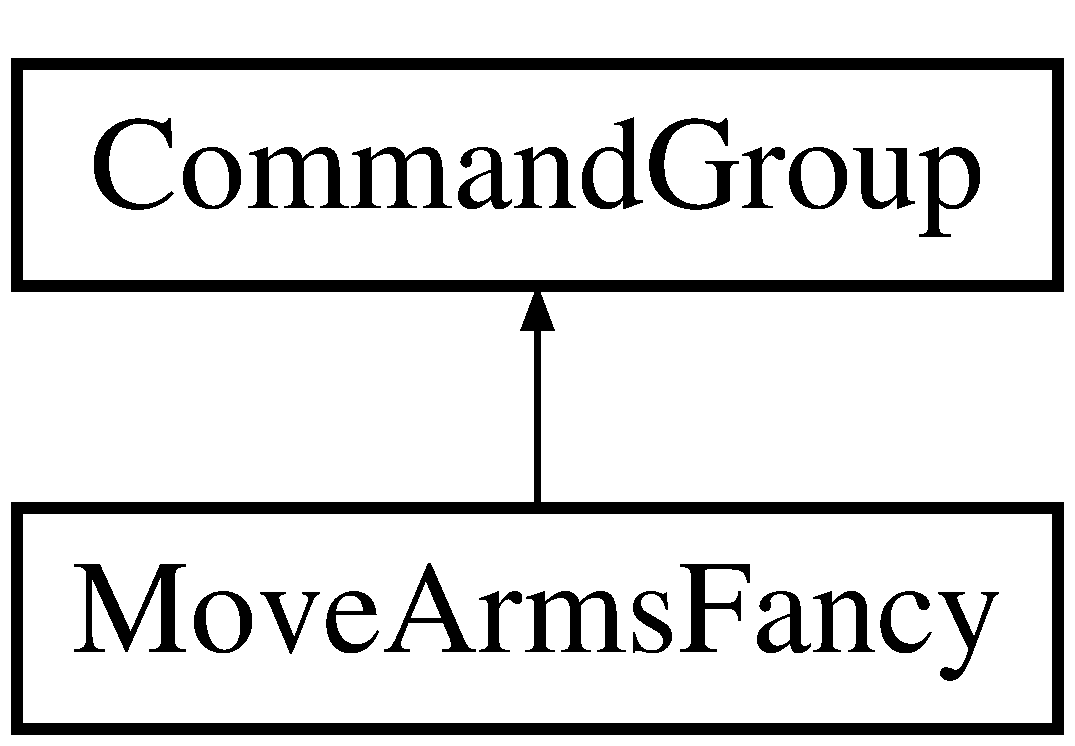
\includegraphics[height=2.000000cm]{class_move_arms_fancy}
\end{center}
\end{figure}
\subsection*{Public Member Functions}
\begin{DoxyCompactItemize}
\item 
\hypertarget{class_move_arms_fancy_ae10b5c866d4d2ae7585ad127a942805e}{}{\bfseries Move\+Arms\+Fancy} (bool up)\label{class_move_arms_fancy_ae10b5c866d4d2ae7585ad127a942805e}

\end{DoxyCompactItemize}


The documentation for this class was generated from the following files\+:\begin{DoxyCompactItemize}
\item 
Cyclophosphamide/src/\+Commands/\+Can\+Collecterino/Move\+Arms\+Fancy.\+h\item 
Cyclophosphamide/src/\+Commands/\+Can\+Collecterino/Move\+Arms\+Fancy.\+cpp\end{DoxyCompactItemize}

\hypertarget{class_move_wrist}{}\section{Move\+Wrist Class Reference}
\label{class_move_wrist}\index{Move\+Wrist@{Move\+Wrist}}


{\ttfamily \#include $<$Move\+Wrist.\+h$>$}

Inheritance diagram for Move\+Wrist\+:\begin{figure}[H]
\begin{center}
\leavevmode
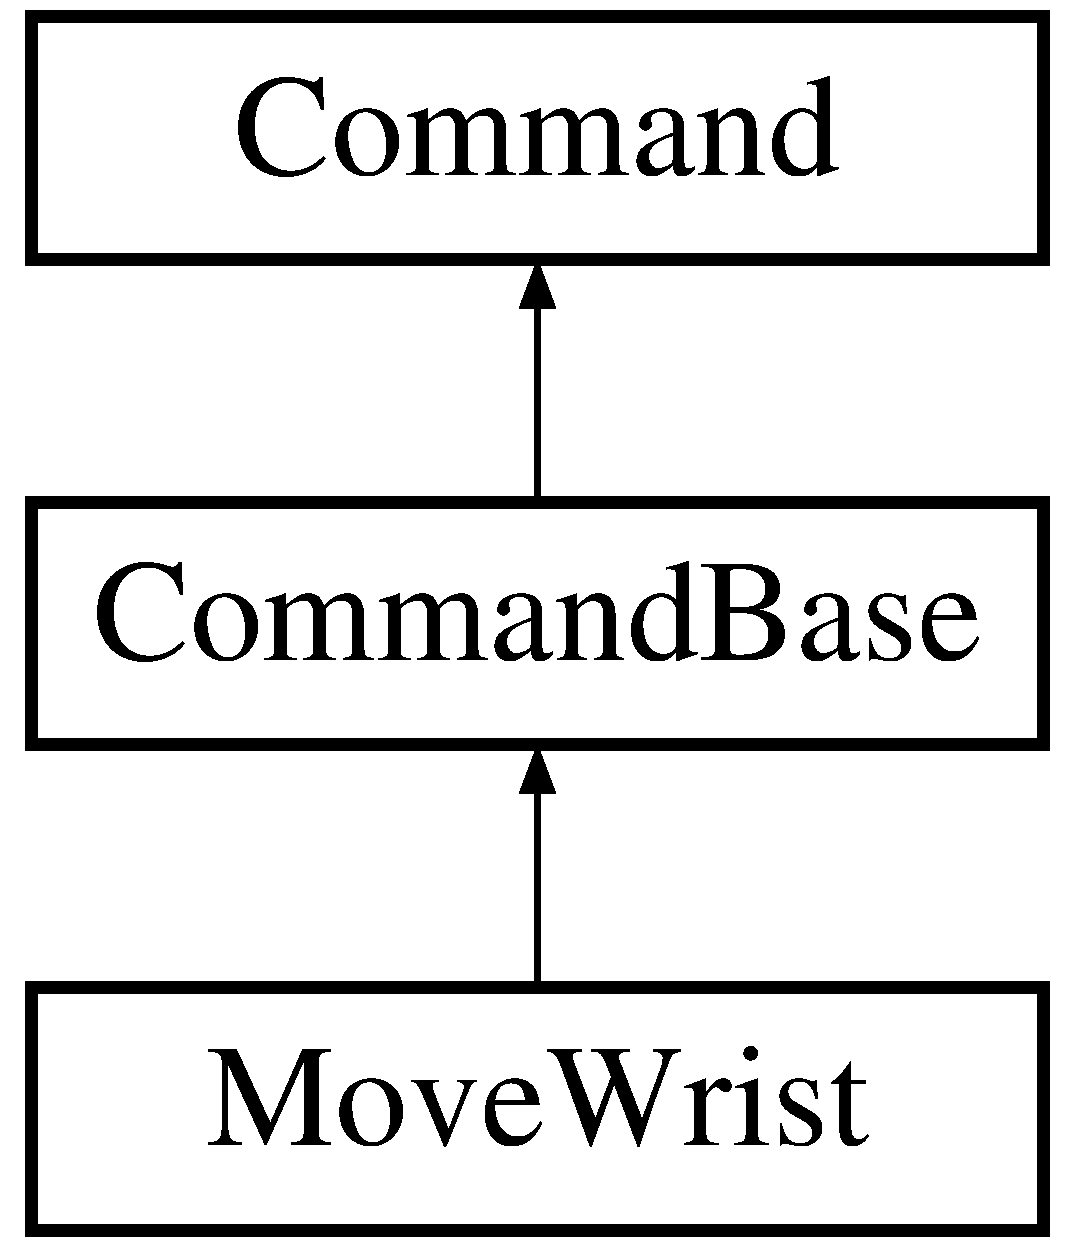
\includegraphics[height=3.000000cm]{class_move_wrist}
\end{center}
\end{figure}
\subsection*{Public Types}
\begin{DoxyCompactItemize}
\item 
\hypertarget{class_move_wrist_a3fdfbb131a8abfcd18962448dabf1dcb}{}enum {\bfseries State} \{ {\bfseries open}, 
{\bfseries close}, 
{\bfseries toggle}
 \}\label{class_move_wrist_a3fdfbb131a8abfcd18962448dabf1dcb}

\end{DoxyCompactItemize}
\subsection*{Public Member Functions}
\begin{DoxyCompactItemize}
\item 
\hypertarget{class_move_wrist_a520569159ba16c6b773306b8d06c6dc2}{}{\bfseries Move\+Wrist} (State state)\label{class_move_wrist_a520569159ba16c6b773306b8d06c6dc2}

\item 
\hypertarget{class_move_wrist_a7b053ffafaef440ebec6b1719474353b}{}void {\bfseries Initialize} ()\label{class_move_wrist_a7b053ffafaef440ebec6b1719474353b}

\item 
\hypertarget{class_move_wrist_a1f38db78ec0dafaa9cfe83cdb5bc133e}{}void {\bfseries Execute} ()\label{class_move_wrist_a1f38db78ec0dafaa9cfe83cdb5bc133e}

\item 
\hypertarget{class_move_wrist_aea1c4b4c5984725cb4302a38850529e8}{}bool {\bfseries Is\+Finished} ()\label{class_move_wrist_aea1c4b4c5984725cb4302a38850529e8}

\item 
\hypertarget{class_move_wrist_a98b40a9310e27fbbead96c0208af0931}{}void {\bfseries End} ()\label{class_move_wrist_a98b40a9310e27fbbead96c0208af0931}

\item 
\hypertarget{class_move_wrist_ad44c5f341795ac74c24b4fc3fcf1db1c}{}void {\bfseries Interrupted} ()\label{class_move_wrist_ad44c5f341795ac74c24b4fc3fcf1db1c}

\end{DoxyCompactItemize}
\subsection*{Additional Inherited Members}


\subsection{Detailed Description}
Toggles the position of the wrists (opened or closed) set the pneumatics to forward else reverse. 

The documentation for this class was generated from the following files\+:\begin{DoxyCompactItemize}
\item 
Cyclophosphamide/src/\+Commands/\+Can\+Collecterino/\+Arms/Move\+Wrist.\+h\item 
Cyclophosphamide/src/\+Commands/\+Can\+Collecterino/\+Arms/Move\+Wrist.\+cpp\end{DoxyCompactItemize}

\hypertarget{class_o_i}{}\section{O\+I Class Reference}
\label{class_o_i}\index{O\+I@{O\+I}}
\subsection*{Public Member Functions}
\begin{DoxyCompactItemize}
\item 
\hypertarget{class_o_i_a44e3993b74e84ff3f42e085bf2339fd3}{}Joystick $\ast$ {\bfseries get\+Joystick\+Left} ()\label{class_o_i_a44e3993b74e84ff3f42e085bf2339fd3}

\item 
\hypertarget{class_o_i_a3e6f636adbcd28305a128c60ed37ca51}{}Joystick $\ast$ {\bfseries get\+Joystick\+Right} ()\label{class_o_i_a3e6f636adbcd28305a128c60ed37ca51}

\item 
\hypertarget{class_o_i_ab94df2d2b7daef071403aaa68f0c2110}{}Joystick $\ast$ {\bfseries get\+Joystick\+Operator} ()\label{class_o_i_ab94df2d2b7daef071403aaa68f0c2110}

\item 
\hypertarget{class_o_i_ab12f69fdde64ee428a470050108f7723}{}double {\bfseries get\+Analog\+Value} (int input)\label{class_o_i_ab12f69fdde64ee428a470050108f7723}

\item 
\hypertarget{class_o_i_a1235966866aa76065043d7f222ac5347}{}bool {\bfseries get\+Unactuate} ()\label{class_o_i_a1235966866aa76065043d7f222ac5347}

\item 
\hypertarget{class_o_i_a30153c1afd5cb73f706423af66587f01}{}void {\bfseries register\+Button\+Listeners} ()\label{class_o_i_a30153c1afd5cb73f706423af66587f01}

\item 
\hypertarget{class_o_i_aabe980a3191aaa7686ca122bb75fa64c}{}bool {\bfseries is\+Joystick\+Button\+Pressed} (bool is\+Left, int val)\label{class_o_i_aabe980a3191aaa7686ca122bb75fa64c}

\item 
\hypertarget{class_o_i_a9b2f26a2a2f61103a6542d147f23444e}{}Joystick $\ast$ {\bfseries get\+Joystick\+Left} ()\label{class_o_i_a9b2f26a2a2f61103a6542d147f23444e}

\item 
\hypertarget{class_o_i_a7fe906ee41761e1c317283c0078de84d}{}Joystick $\ast$ {\bfseries get\+Joystick\+Right} ()\label{class_o_i_a7fe906ee41761e1c317283c0078de84d}

\item 
\hypertarget{class_o_i_a30153c1afd5cb73f706423af66587f01}{}void {\bfseries register\+Button\+Listeners} ()\label{class_o_i_a30153c1afd5cb73f706423af66587f01}

\end{DoxyCompactItemize}
\subsection*{Public Attributes}
\begin{DoxyCompactItemize}
\item 
\hypertarget{class_o_i_a2bee2d865aa653e059b603ce820c26dc}{}Joystick $\ast$ {\bfseries joystick\+Left}\label{class_o_i_a2bee2d865aa653e059b603ce820c26dc}

\item 
\hypertarget{class_o_i_aaaafd946afb55b9d9404afe89a705fd5}{}Joystick $\ast$ {\bfseries joystick\+Right}\label{class_o_i_aaaafd946afb55b9d9404afe89a705fd5}

\item 
\hypertarget{class_o_i_a2fc95d5844f23524dd94f564eef2391b}{}Joystick $\ast$ {\bfseries joystick\+Operator}\label{class_o_i_a2fc95d5844f23524dd94f564eef2391b}

\item 
\hypertarget{class_o_i_adff52f1cc6091a586837550a05c77971}{}Joystick\+Button $\ast$ {\bfseries push\+Toggle}\label{class_o_i_adff52f1cc6091a586837550a05c77971}

\item 
\hypertarget{class_o_i_ab02cd0377621491441c4f7418ca10f62}{}Joystick\+Button $\ast$ {\bfseries pull\+Button}\label{class_o_i_ab02cd0377621491441c4f7418ca10f62}

\item 
\hypertarget{class_o_i_a7943df53f2f363fc651678f5e43aaa8c}{}Joystick\+Button $\ast$ {\bfseries tote\+Intake\+Button\+Forward}\label{class_o_i_a7943df53f2f363fc651678f5e43aaa8c}

\item 
\hypertarget{class_o_i_a5924e02ee1bf7b6c82c644e637b9bfce}{}Joystick\+Button $\ast$ {\bfseries move\+Arms\+Down}\label{class_o_i_a5924e02ee1bf7b6c82c644e637b9bfce}

\item 
\hypertarget{class_o_i_ab6757fb5ca25809e06d87890075fd6b4}{}Joystick\+Button $\ast$ {\bfseries left\+Load\+Button}\label{class_o_i_ab6757fb5ca25809e06d87890075fd6b4}

\item 
\hypertarget{class_o_i_a767feac46732443432a500c3a9b6c1f5}{}Joystick\+Button $\ast$ {\bfseries right\+Load\+Button}\label{class_o_i_a767feac46732443432a500c3a9b6c1f5}

\item 
\hypertarget{class_o_i_ae8d9bbb4b6fc16b8ff7a386b55795dcb}{}Joystick\+Button $\ast$ {\bfseries tote\+Lifter\+Up}\label{class_o_i_ae8d9bbb4b6fc16b8ff7a386b55795dcb}

\item 
\hypertarget{class_o_i_ad63f1e29bf862c03f710c422e0ba277e}{}Joystick\+Button $\ast$ {\bfseries tote\+Lifter\+Down}\label{class_o_i_ad63f1e29bf862c03f710c422e0ba277e}

\item 
\hypertarget{class_o_i_ad776b494657e4519dc8ef40fa7a55e54}{}Joystick\+Button $\ast$ {\bfseries tote\+Lifter\+Floor}\label{class_o_i_ad776b494657e4519dc8ef40fa7a55e54}

\item 
\hypertarget{class_o_i_a83df52f98c7df1592fad457c1c9018d1}{}Joystick\+Button $\ast$ {\bfseries tote\+Lifter\+Carry}\label{class_o_i_a83df52f98c7df1592fad457c1c9018d1}

\item 
\hypertarget{class_o_i_a0325e7b2a9652cd9a88675ae14948c0d}{}Joystick\+Button $\ast$ {\bfseries tote\+Lifter\+Lift}\label{class_o_i_a0325e7b2a9652cd9a88675ae14948c0d}

\item 
\hypertarget{class_o_i_a1fdfdcc5b5a1357eeecedc82a57c5085}{}Joystick\+Button $\ast$ {\bfseries move\+Arms\+Up}\label{class_o_i_a1fdfdcc5b5a1357eeecedc82a57c5085}

\item 
\hypertarget{class_o_i_a13093d5cb6fd46b3b7e265e24d9ff733}{}Joystick\+Button $\ast$ {\bfseries move\+Arms\+Knock}\label{class_o_i_a13093d5cb6fd46b3b7e265e24d9ff733}

\item 
\hypertarget{class_o_i_a52f4550ea9f788301cf5f77ffd406612}{}Joystick\+Button $\ast$ {\bfseries collect}\label{class_o_i_a52f4550ea9f788301cf5f77ffd406612}

\item 
\hypertarget{class_o_i_a73cafce878fd10b6a5543e029606f559}{}Joystick\+Button $\ast$ {\bfseries wrist\+Open}\label{class_o_i_a73cafce878fd10b6a5543e029606f559}

\item 
\hypertarget{class_o_i_ae3ffffcf8b54b38f13faf50a154aceb9}{}Joystick\+Button $\ast$ {\bfseries wrist\+Close}\label{class_o_i_ae3ffffcf8b54b38f13faf50a154aceb9}

\end{DoxyCompactItemize}


The documentation for this class was generated from the following files\+:\begin{DoxyCompactItemize}
\item 
Cyclophosphamide/src/O\+I.\+h\item 
Cyclophosphamide/src/O\+I.\+cpp\end{DoxyCompactItemize}

\hypertarget{class_omega_supreme}{}\section{Omega\+Supreme Class Reference}
\label{class_omega_supreme}\index{Omega\+Supreme@{Omega\+Supreme}}
Inheritance diagram for Omega\+Supreme\+:\begin{figure}[H]
\begin{center}
\leavevmode
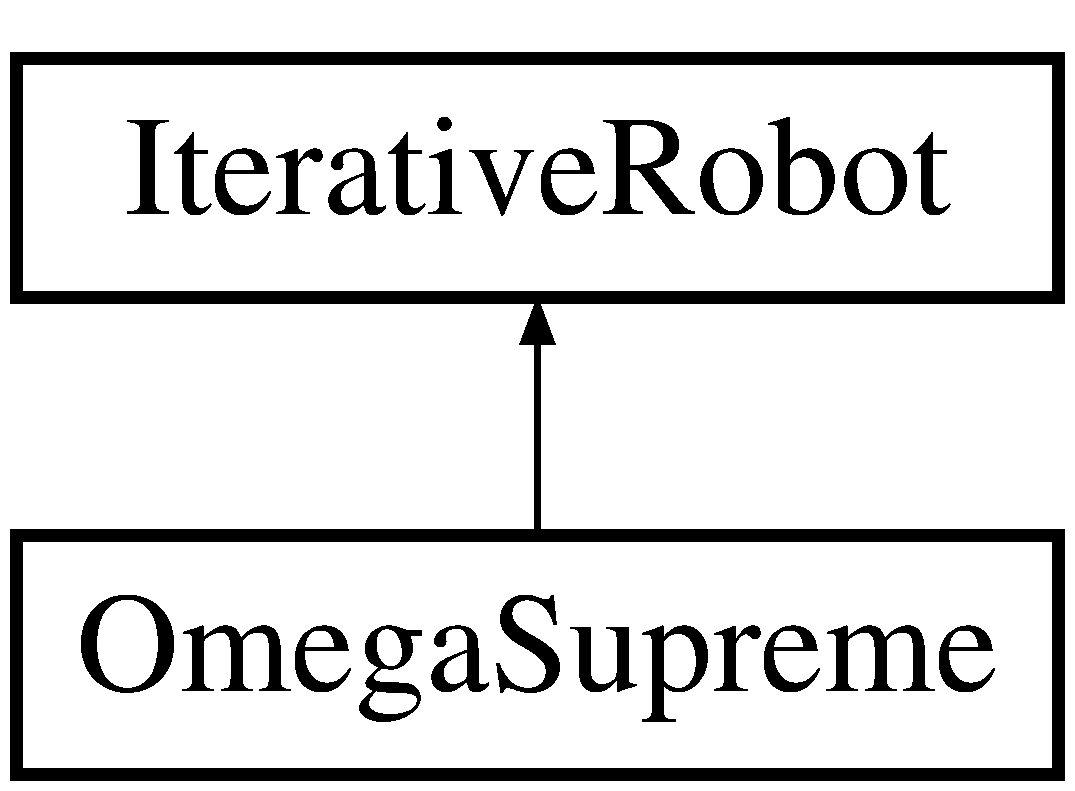
\includegraphics[height=2.000000cm]{class_omega_supreme}
\end{center}
\end{figure}
\subsection*{Public Member Functions}
\begin{DoxyCompactItemize}
\item 
\hypertarget{class_omega_supreme_a482ca0a74da81753c74370a7e87d1648}{}virtual void {\bfseries Robot\+Init} ()\label{class_omega_supreme_a482ca0a74da81753c74370a7e87d1648}

\item 
\hypertarget{class_omega_supreme_a90b13863e87bcb023e3d17da3da64de3}{}virtual void {\bfseries Autonomous\+Init} ()\label{class_omega_supreme_a90b13863e87bcb023e3d17da3da64de3}

\item 
\hypertarget{class_omega_supreme_af61caca5d9dc88aaaaff05a129e2c5cc}{}virtual void {\bfseries Autonomous\+Periodic} ()\label{class_omega_supreme_af61caca5d9dc88aaaaff05a129e2c5cc}

\item 
\hypertarget{class_omega_supreme_a63020edb1ab98ac912df92b99bb02618}{}virtual void {\bfseries Teleop\+Init} ()\label{class_omega_supreme_a63020edb1ab98ac912df92b99bb02618}

\item 
\hypertarget{class_omega_supreme_a70ba01219fd7d9cea9c11856146ca1d3}{}virtual void {\bfseries Teleop\+Periodic} ()\label{class_omega_supreme_a70ba01219fd7d9cea9c11856146ca1d3}

\item 
\hypertarget{class_omega_supreme_ab1974ba070c3b095e2e49b1372e8f3bc}{}virtual void {\bfseries Test\+Init} ()\label{class_omega_supreme_ab1974ba070c3b095e2e49b1372e8f3bc}

\item 
\hypertarget{class_omega_supreme_ab410619ec5070b06a26ba9ad42458e4b}{}virtual void {\bfseries Test\+Periodic} ()\label{class_omega_supreme_ab410619ec5070b06a26ba9ad42458e4b}

\item 
\hypertarget{class_omega_supreme_a13f930ffdaac6e4a9d16cd94623b8e32}{}virtual void {\bfseries Disabled\+Init} ()\label{class_omega_supreme_a13f930ffdaac6e4a9d16cd94623b8e32}

\item 
\hypertarget{class_omega_supreme_ac9c5876cc5178fa49e1654689264b08e}{}void {\bfseries Watch\+Dogg} ()\label{class_omega_supreme_ac9c5876cc5178fa49e1654689264b08e}

\end{DoxyCompactItemize}


The documentation for this class was generated from the following files\+:\begin{DoxyCompactItemize}
\item 
Cyclophosphamide/src/Omega\+Supreme.\+h\item 
Cyclophosphamide/src/Omega\+Supreme.\+cpp\end{DoxyCompactItemize}

\hypertarget{class_override_gyro}{}\section{Override\+Gyro Class Reference}
\label{class_override_gyro}\index{Override\+Gyro@{Override\+Gyro}}
Inheritance diagram for Override\+Gyro\+:\begin{figure}[H]
\begin{center}
\leavevmode
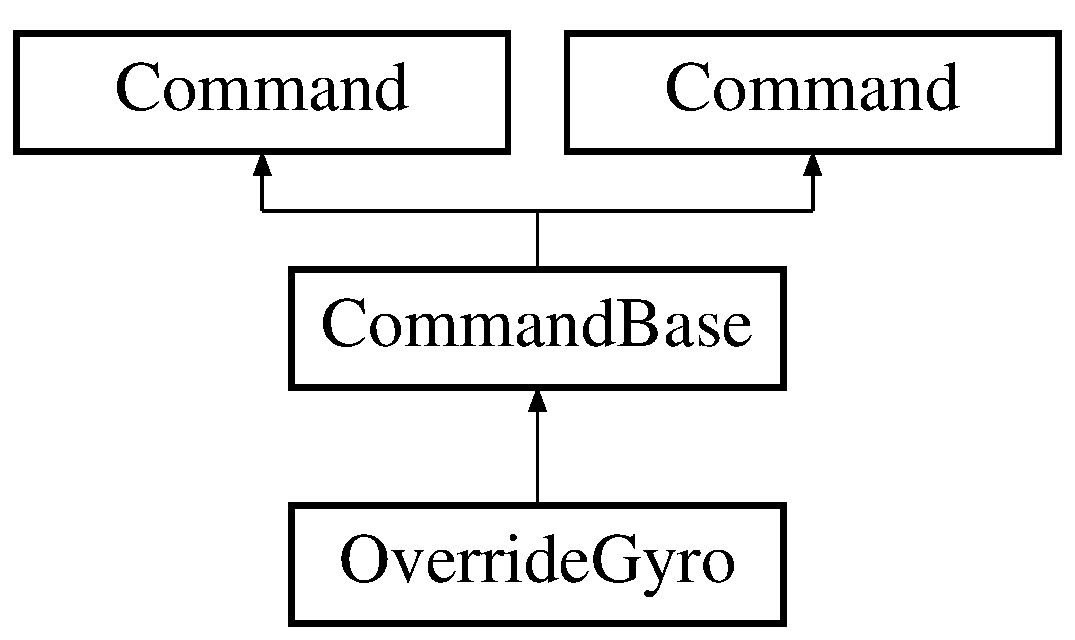
\includegraphics[height=3.000000cm]{class_override_gyro}
\end{center}
\end{figure}
\subsection*{Public Member Functions}
\begin{DoxyCompactItemize}
\item 
\hypertarget{class_override_gyro_ac78f181f557774ea3b77c179fb01e9b5}{}{\bfseries Override\+Gyro} (bool override)\label{class_override_gyro_ac78f181f557774ea3b77c179fb01e9b5}

\item 
\hypertarget{class_override_gyro_a9d1af5c68f2c1fdfebd7bd90f1a4f3ae}{}void {\bfseries Initialize} ()\label{class_override_gyro_a9d1af5c68f2c1fdfebd7bd90f1a4f3ae}

\item 
\hypertarget{class_override_gyro_a9fa5bb1db7ef8eae36207f547674ae5b}{}void {\bfseries Execute} ()\label{class_override_gyro_a9fa5bb1db7ef8eae36207f547674ae5b}

\item 
\hypertarget{class_override_gyro_a44fe43c8215245cd31c569e8953f1ed3}{}bool {\bfseries Is\+Finished} ()\label{class_override_gyro_a44fe43c8215245cd31c569e8953f1ed3}

\item 
\hypertarget{class_override_gyro_a0d6e3c1f8476ef339b12f2d44b5450f4}{}void {\bfseries End} ()\label{class_override_gyro_a0d6e3c1f8476ef339b12f2d44b5450f4}

\item 
\hypertarget{class_override_gyro_aaca558864ff872cdcebb9e5f82511bbb}{}void {\bfseries Interrupted} ()\label{class_override_gyro_aaca558864ff872cdcebb9e5f82511bbb}

\end{DoxyCompactItemize}
\subsection*{Additional Inherited Members}


The documentation for this class was generated from the following files\+:\begin{DoxyCompactItemize}
\item 
Cyclophosphamide/src/\+Commands/\+Drivebase/Override\+Gyro.\+h\item 
Cyclophosphamide/src/\+Commands/\+Drivebase/Override\+Gyro.\+cpp\end{DoxyCompactItemize}

\hypertarget{class_put_up}{}\section{Put\+Up Class Reference}
\label{class_put_up}\index{Put\+Up@{Put\+Up}}
Inheritance diagram for Put\+Up\+:\begin{figure}[H]
\begin{center}
\leavevmode
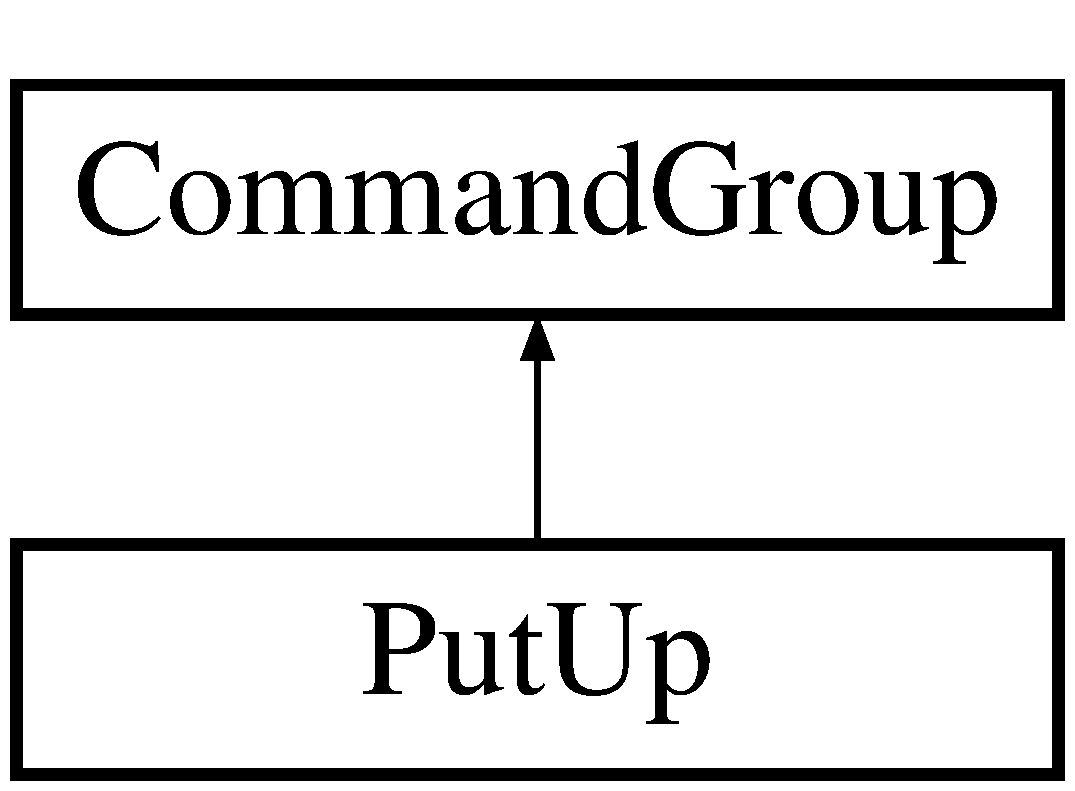
\includegraphics[height=2.000000cm]{class_put_up}
\end{center}
\end{figure}
\subsection*{Public Member Functions}
\begin{DoxyCompactItemize}
\item 
\hyperlink{class_put_up_a74d9b5583b43c5331cb49801f1b0e35b}{Put\+Up} ()
\end{DoxyCompactItemize}


\subsection{Constructor \& Destructor Documentation}
\hypertarget{class_put_up_a74d9b5583b43c5331cb49801f1b0e35b}{}\index{Put\+Up@{Put\+Up}!Put\+Up@{Put\+Up}}
\index{Put\+Up@{Put\+Up}!Put\+Up@{Put\+Up}}
\subsubsection[{Put\+Up}]{\setlength{\rightskip}{0pt plus 5cm}Put\+Up\+::\+Put\+Up (
\begin{DoxyParamCaption}
{}
\end{DoxyParamCaption}
)}\label{class_put_up_a74d9b5583b43c5331cb49801f1b0e35b}
Sets the arms of the cancollecterino to a vertical position 

The documentation for this class was generated from the following file\+:\begin{DoxyCompactItemize}
\item 
Cyclophosphamide/src/\+Commands/\+Can\+Collecterino/Put\+Up.\+h\end{DoxyCompactItemize}

\hypertarget{class_reset_elevator_encoder}{}\section{Reset\+Elevator\+Encoder Class Reference}
\label{class_reset_elevator_encoder}\index{Reset\+Elevator\+Encoder@{Reset\+Elevator\+Encoder}}
Inheritance diagram for Reset\+Elevator\+Encoder\+:\begin{figure}[H]
\begin{center}
\leavevmode
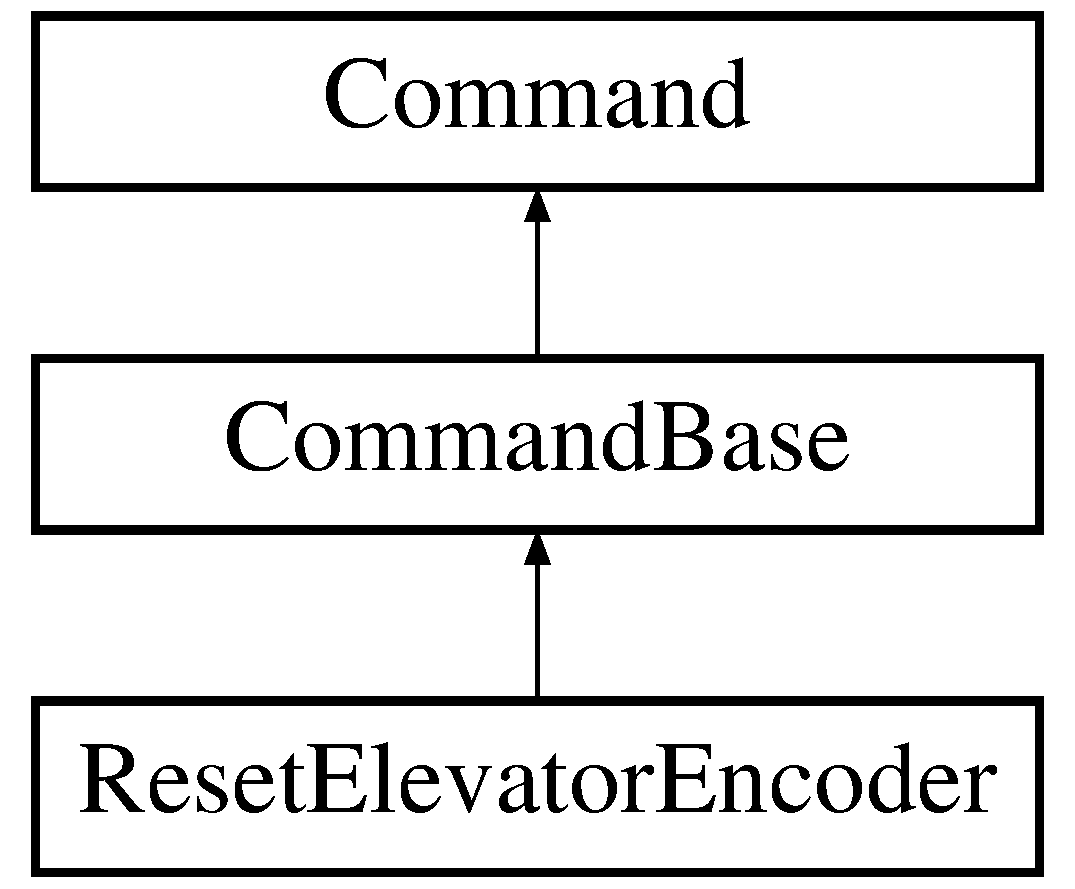
\includegraphics[height=3.000000cm]{class_reset_elevator_encoder}
\end{center}
\end{figure}
\subsection*{Public Member Functions}
\begin{DoxyCompactItemize}
\item 
\hypertarget{class_reset_elevator_encoder_a0e3a40d24f7a0a96f631599099164745}{}void {\bfseries Initialize} ()\label{class_reset_elevator_encoder_a0e3a40d24f7a0a96f631599099164745}

\item 
\hypertarget{class_reset_elevator_encoder_a924742c61f49ffa9b1d2c2706e994091}{}void {\bfseries Execute} ()\label{class_reset_elevator_encoder_a924742c61f49ffa9b1d2c2706e994091}

\item 
\hypertarget{class_reset_elevator_encoder_af47be14b74b7d8c1fd339e6e36ebd127}{}bool {\bfseries Is\+Finished} ()\label{class_reset_elevator_encoder_af47be14b74b7d8c1fd339e6e36ebd127}

\item 
\hypertarget{class_reset_elevator_encoder_af256e1346b89aad463aeb591a40226f3}{}void {\bfseries End} ()\label{class_reset_elevator_encoder_af256e1346b89aad463aeb591a40226f3}

\item 
\hypertarget{class_reset_elevator_encoder_a6ffbbbeffbb11266d7ac68bf26877794}{}void {\bfseries Interrupted} ()\label{class_reset_elevator_encoder_a6ffbbbeffbb11266d7ac68bf26877794}

\end{DoxyCompactItemize}
\subsection*{Additional Inherited Members}


The documentation for this class was generated from the following files\+:\begin{DoxyCompactItemize}
\item 
Cyclophosphamide/src/\+Commands/\+Tote\+Lifting/zeroing/Reset\+Elevator\+Encoder.\+h\item 
Cyclophosphamide/src/\+Commands/\+Tote\+Lifting/zeroing/Reset\+Elevator\+Encoder.\+cpp\end{DoxyCompactItemize}

\hypertarget{class_safe_down_up}{}\section{Safe\+Down\+Up Class Reference}
\label{class_safe_down_up}\index{Safe\+Down\+Up@{Safe\+Down\+Up}}
Inheritance diagram for Safe\+Down\+Up\+:\begin{figure}[H]
\begin{center}
\leavevmode
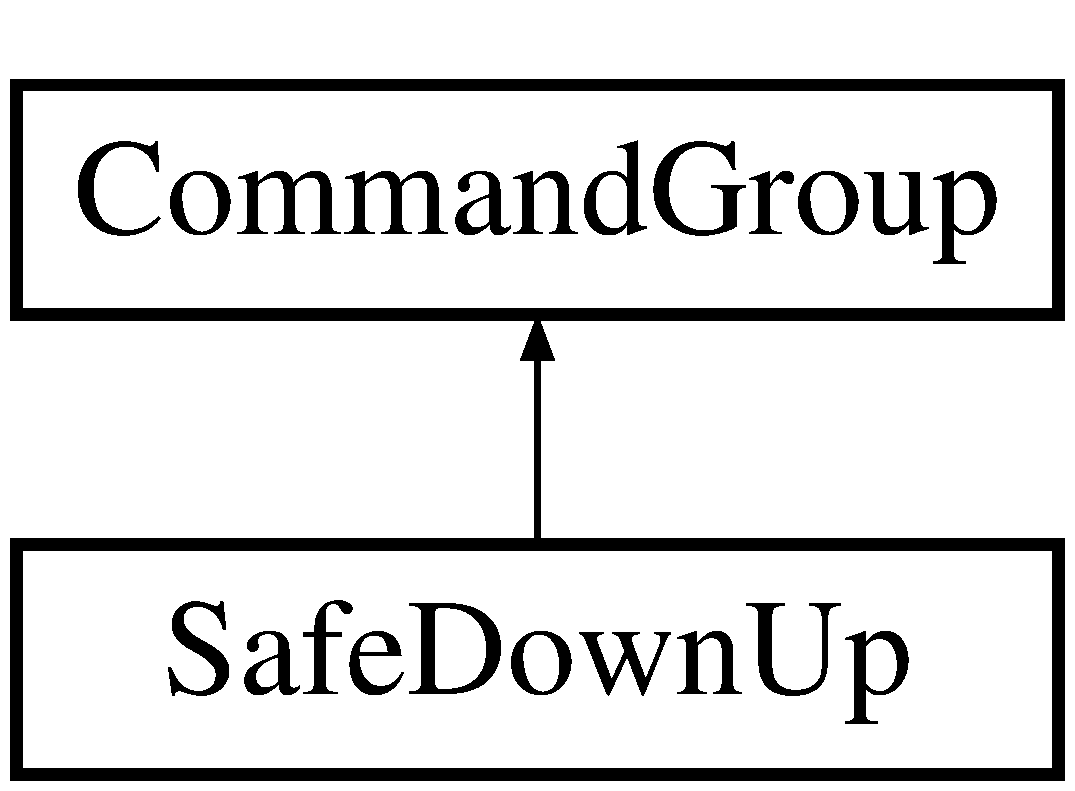
\includegraphics[height=2.000000cm]{class_safe_down_up}
\end{center}
\end{figure}
\subsection*{Public Member Functions}
\begin{DoxyCompactItemize}
\item 
\hypertarget{class_safe_down_up_a950bd9713f2f5f726413041dc356c089}{}{\bfseries Safe\+Down\+Up} (Down\+Up\+::\+Position pos)\label{class_safe_down_up_a950bd9713f2f5f726413041dc356c089}

\end{DoxyCompactItemize}


The documentation for this class was generated from the following files\+:\begin{DoxyCompactItemize}
\item 
Cyclophosphamide/src/\+Commands/\+Tote\+Lifting/Safe\+Down\+Up.\+h\item 
Cyclophosphamide/src/\+Commands/\+Tote\+Lifting/Safe\+Down\+Up.\+cpp\end{DoxyCompactItemize}

\hypertarget{class_safe_lift_to_height}{}\section{Safe\+Lift\+To\+Height Class Reference}
\label{class_safe_lift_to_height}\index{Safe\+Lift\+To\+Height@{Safe\+Lift\+To\+Height}}
Inheritance diagram for Safe\+Lift\+To\+Height\+:\begin{figure}[H]
\begin{center}
\leavevmode
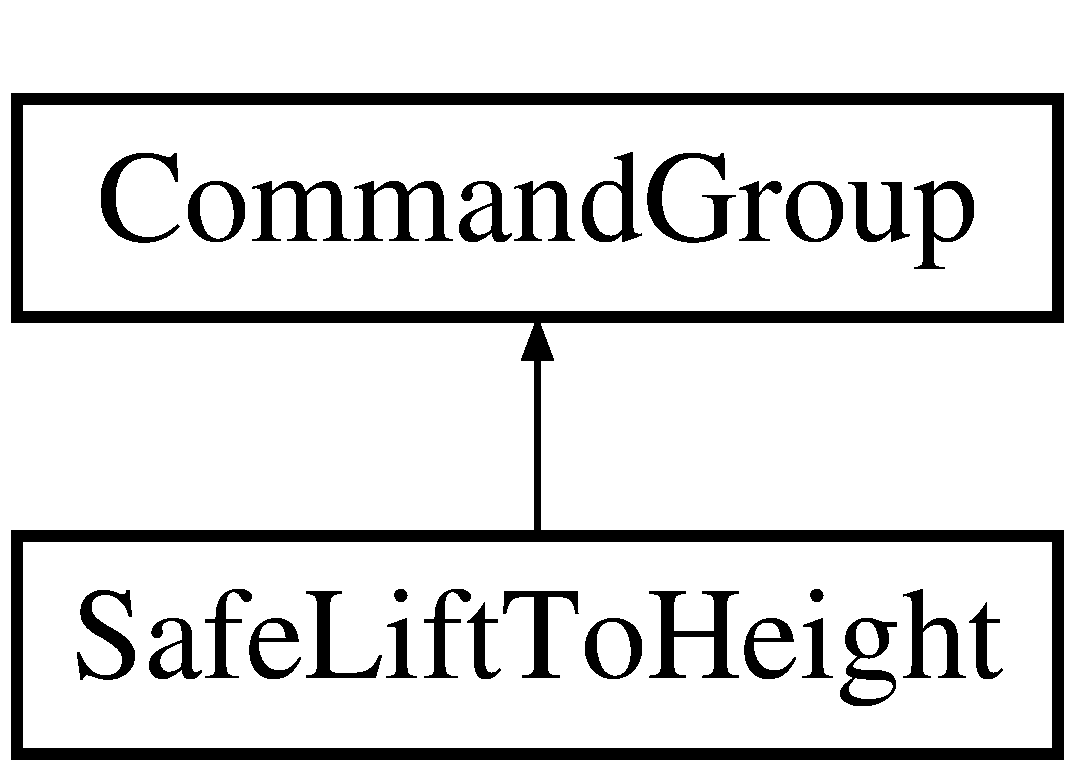
\includegraphics[height=2.000000cm]{class_safe_lift_to_height}
\end{center}
\end{figure}
\subsection*{Public Member Functions}
\begin{DoxyCompactItemize}
\item 
\hypertarget{class_safe_lift_to_height_a165f933574d622580c6e2813286fec2b}{}{\bfseries Safe\+Lift\+To\+Height} (double destination, bool is\+Craaaw\+Safe=false)\label{class_safe_lift_to_height_a165f933574d622580c6e2813286fec2b}

\end{DoxyCompactItemize}


The documentation for this class was generated from the following files\+:\begin{DoxyCompactItemize}
\item 
Cyclophosphamide/src/\+Commands/\+Tote\+Lifting/Safe\+Lift\+To\+Height.\+h\item 
Cyclophosphamide/src/\+Commands/\+Tote\+Lifting/Safe\+Lift\+To\+Height.\+cpp\end{DoxyCompactItemize}

\hypertarget{class_score}{}\section{Score Class Reference}
\label{class_score}\index{Score@{Score}}
Inheritance diagram for Score\+:\begin{figure}[H]
\begin{center}
\leavevmode
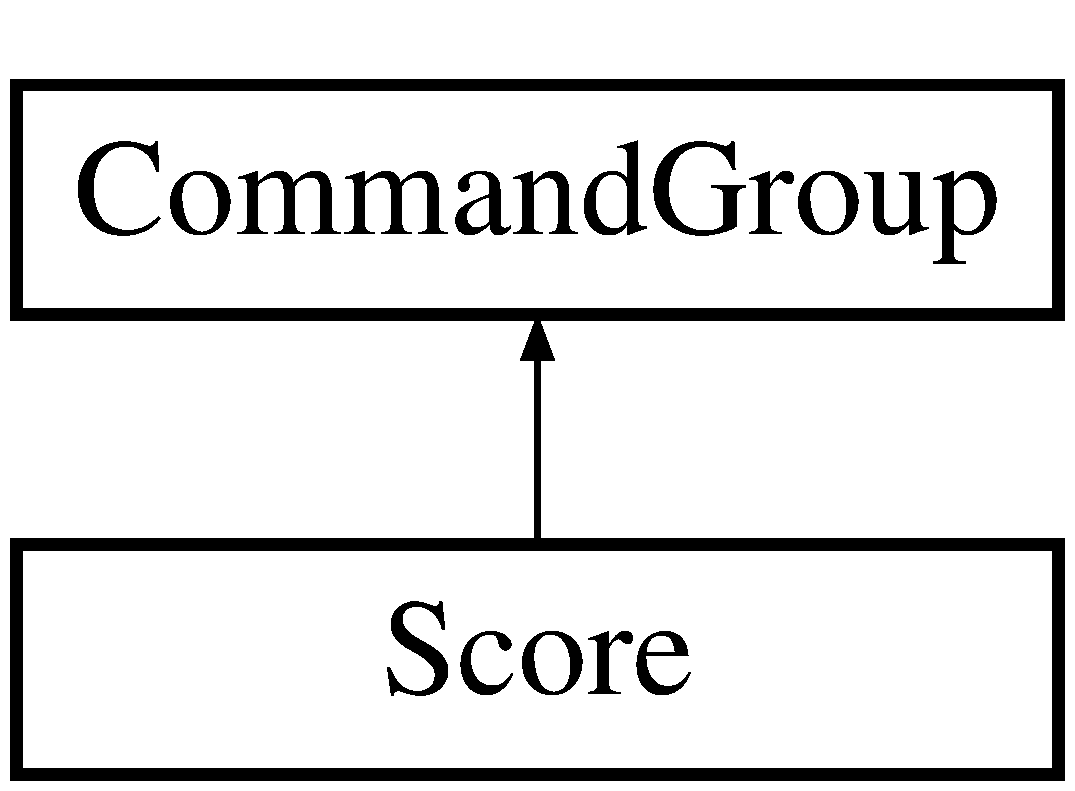
\includegraphics[height=2.000000cm]{class_score}
\end{center}
\end{figure}


The documentation for this class was generated from the following files\+:\begin{DoxyCompactItemize}
\item 
Cyclophosphamide/src/\+Commands/Score.\+h\item 
Cyclophosphamide/src/\+Commands/Score.\+cpp\end{DoxyCompactItemize}

\hypertarget{class_script_command}{}\section{Script\+Command Class Reference}
\label{class_script_command}\index{Script\+Command@{Script\+Command}}


{\ttfamily \#include $<$Scripting.\+h$>$}

Inheritance diagram for Script\+Command\+:\begin{figure}[H]
\begin{center}
\leavevmode
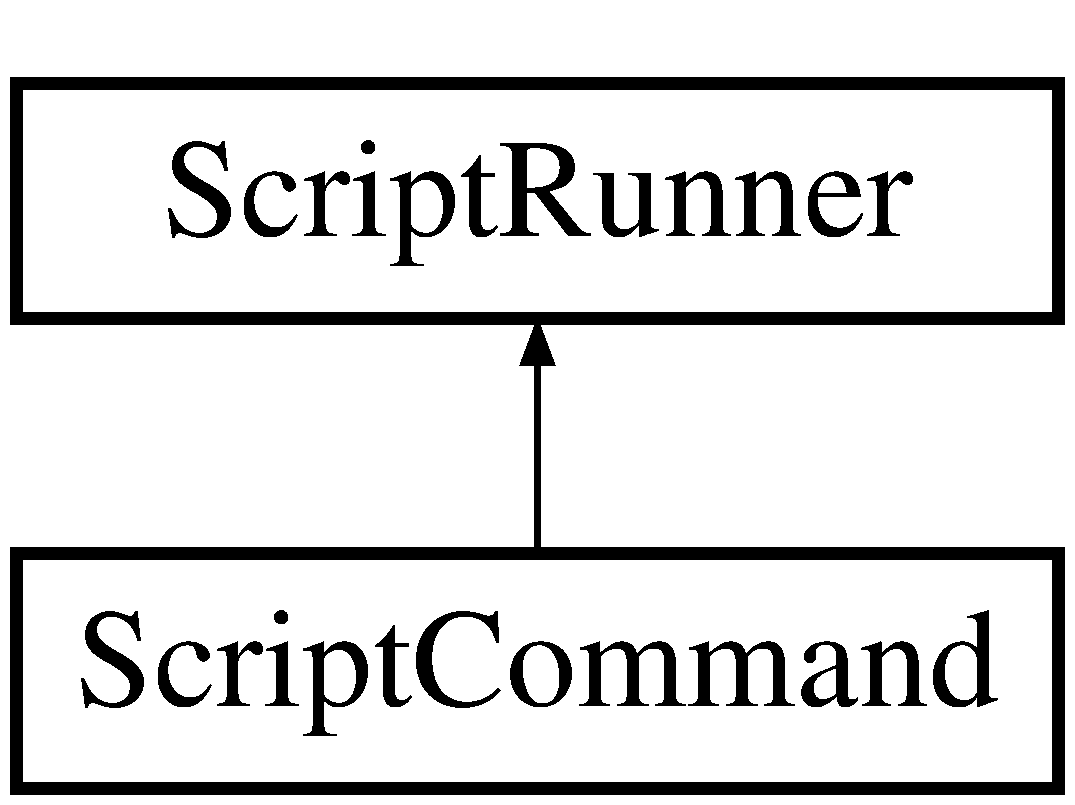
\includegraphics[height=2.000000cm]{class_script_command}
\end{center}
\end{figure}
\subsection*{Public Member Functions}
\begin{DoxyCompactItemize}
\item 
\hypertarget{class_script_command_aff7321091c96a2bef01c8756882feb2f}{}{\bfseries Script\+Command} (Command $\ast$start)\label{class_script_command_aff7321091c96a2bef01c8756882feb2f}

\item 
\hypertarget{class_script_command_a69cf76011e926f7bb491684306a6c328}{}virtual void {\bfseries start\+Command} ()\label{class_script_command_a69cf76011e926f7bb491684306a6c328}

\end{DoxyCompactItemize}


\subsection{Detailed Description}
Starts an arbitrary command with the command parameter. 

The documentation for this class was generated from the following files\+:\begin{DoxyCompactItemize}
\item 
Cyclophosphamide/src/\+Commands/\+Autonomous/Scripting.\+h\item 
Cyclophosphamide/src/\+Commands/\+Autonomous/Scripting.\+cpp\end{DoxyCompactItemize}

\hypertarget{class_scripting}{}\section{Scripting Class Reference}
\label{class_scripting}\index{Scripting@{Scripting}}
\subsection*{Static Public Member Functions}
\begin{DoxyCompactItemize}
\item 
static char $\ast$ \hyperlink{class_scripting_ab94dec041f116a92d48c8b28e3f086c0}{read\+From\+File} (char $\ast$file, int \&size)
\begin{DoxyCompactList}\small\item\em Returns a file\textquotesingle{}s contents. \end{DoxyCompactList}\item 
static \hyperlink{class_autonomous}{Autonomous} $\ast$ \hyperlink{class_scripting_a95d3be53b7e0dd29d434937cf57c928e}{create\+Command} (int size, char $\ast$raw\+Data)
\begin{DoxyCompactList}\small\item\em Creates an \hyperlink{class_autonomous}{Autonomous} command. \end{DoxyCompactList}\item 
static Sendable\+Chooser $\ast$ \hyperlink{class_scripting_abef2e025e053a76c5b2ce8115997162b}{generate\+Autonomous\+Modes} (char $\ast$script\+Locations)
\begin{DoxyCompactList}\small\item\em Creates a Sendable\+Chooser from a folder of autonomous files. \end{DoxyCompactList}\end{DoxyCompactItemize}


\subsection{Member Function Documentation}
\hypertarget{class_scripting_a95d3be53b7e0dd29d434937cf57c928e}{}\index{Scripting@{Scripting}!create\+Command@{create\+Command}}
\index{create\+Command@{create\+Command}!Scripting@{Scripting}}
\subsubsection[{create\+Command}]{\setlength{\rightskip}{0pt plus 5cm}{\bf Autonomous} $\ast$ Scripting\+::create\+Command (
\begin{DoxyParamCaption}
\item[{int}]{size, }
\item[{char $\ast$}]{raw\+Data}
\end{DoxyParamCaption}
)\hspace{0.3cm}{\ttfamily [static]}}\label{class_scripting_a95d3be53b7e0dd29d434937cf57c928e}


Creates an \hyperlink{class_autonomous}{Autonomous} command. 

Returns an \hyperlink{class_autonomous}{Autonomous} command based on the contents of raw\+Data 
\begin{DoxyParams}{Parameters}
{\em size} & Size of raw\+Data \\
\hline
{\em raw\+Data} & Raw string containing commands \\
\hline
\end{DoxyParams}
\begin{DoxyReturn}{Returns}
New \hyperlink{class_autonomous}{Autonomous} command 
\end{DoxyReturn}
\hypertarget{class_scripting_abef2e025e053a76c5b2ce8115997162b}{}\index{Scripting@{Scripting}!generate\+Autonomous\+Modes@{generate\+Autonomous\+Modes}}
\index{generate\+Autonomous\+Modes@{generate\+Autonomous\+Modes}!Scripting@{Scripting}}
\subsubsection[{generate\+Autonomous\+Modes}]{\setlength{\rightskip}{0pt plus 5cm}Sendable\+Chooser $\ast$ Scripting\+::generate\+Autonomous\+Modes (
\begin{DoxyParamCaption}
\item[{char $\ast$}]{script\+Locations}
\end{DoxyParamCaption}
)\hspace{0.3cm}{\ttfamily [static]}}\label{class_scripting_abef2e025e053a76c5b2ce8115997162b}


Creates a Sendable\+Chooser from a folder of autonomous files. 

Creates a Sendable\+Chooser. The options are all of the files in the locations folder. Calling Get\+Selected returns a char array, which is the absolute path of the file selected. 
\begin{DoxyParams}{Parameters}
{\em script\+Locations} & The absolute path to the folder containing script locations. Requries trailing slash \\
\hline
\end{DoxyParams}
\begin{DoxyReturn}{Returns}
The Sendable\+Chooser (Get\+Selected returns a char array) 
\end{DoxyReturn}
\hypertarget{class_scripting_ab94dec041f116a92d48c8b28e3f086c0}{}\index{Scripting@{Scripting}!read\+From\+File@{read\+From\+File}}
\index{read\+From\+File@{read\+From\+File}!Scripting@{Scripting}}
\subsubsection[{read\+From\+File}]{\setlength{\rightskip}{0pt plus 5cm}char $\ast$ Scripting\+::read\+From\+File (
\begin{DoxyParamCaption}
\item[{char $\ast$}]{file, }
\item[{int \&}]{size}
\end{DoxyParamCaption}
)\hspace{0.3cm}{\ttfamily [static]}}\label{class_scripting_ab94dec041f116a92d48c8b28e3f086c0}


Returns a file\textquotesingle{}s contents. 

Returns a char array containing the contents of the location file. size is modified by the function to return the size of the file. 
\begin{DoxyParams}{Parameters}
{\em file} & Location of the file \\
\hline
{\em size} & Is modified by the function to return the file size. \\
\hline
\end{DoxyParams}
\begin{DoxyReturn}{Returns}
File contents 
\end{DoxyReturn}


The documentation for this class was generated from the following files\+:\begin{DoxyCompactItemize}
\item 
Cyclophosphamide/src/\+Commands/\+Autonomous/Scripting.\+h\item 
Cyclophosphamide/src/\+Commands/\+Autonomous/Scripting.\+cpp\end{DoxyCompactItemize}

\hypertarget{class_script_loader}{}\section{Script\+Loader Class Reference}
\label{class_script_loader}\index{Script\+Loader@{Script\+Loader}}


{\ttfamily \#include $<$Scripting.\+h$>$}

Inheritance diagram for Script\+Loader\+:\begin{figure}[H]
\begin{center}
\leavevmode
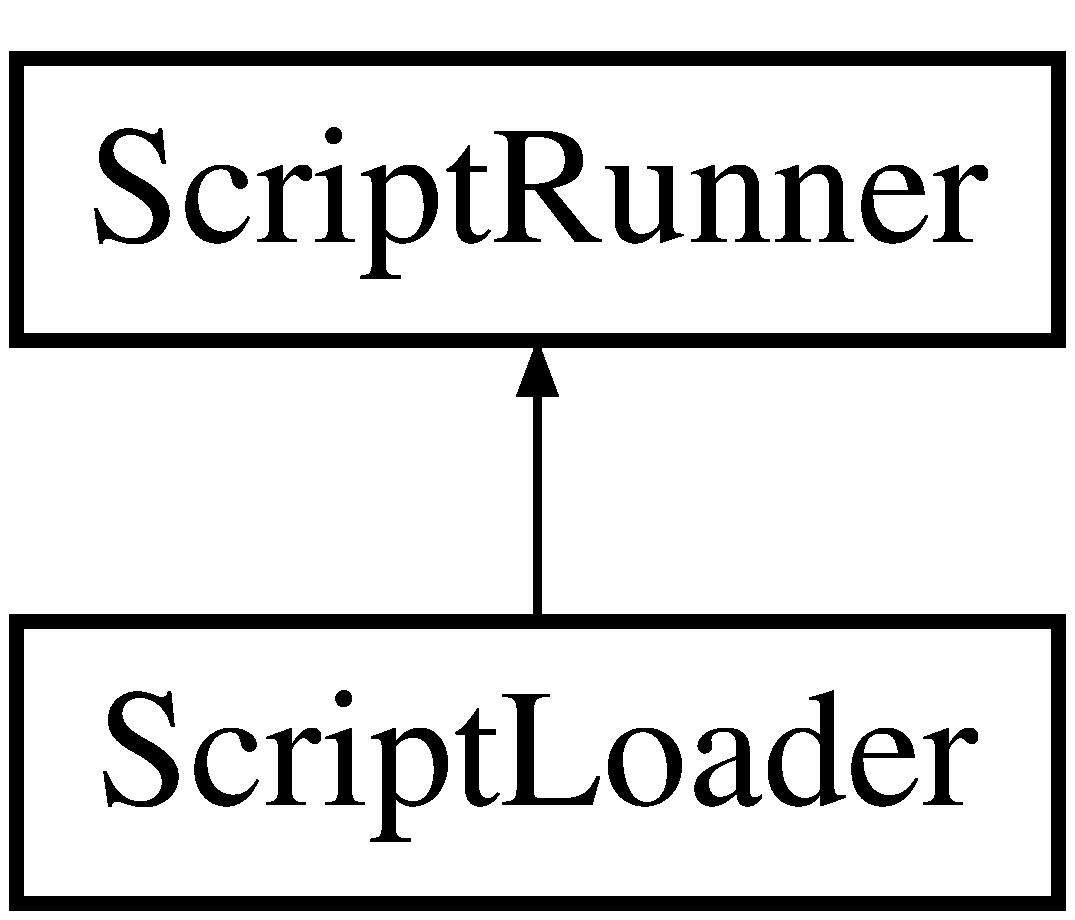
\includegraphics[height=2.000000cm]{class_script_loader}
\end{center}
\end{figure}
\subsection*{Public Member Functions}
\begin{DoxyCompactItemize}
\item 
\hypertarget{class_script_loader_ac93edaa9f08c4db68656111f7a67ed33}{}{\bfseries Script\+Loader} (char $\ast$f\+Name)\label{class_script_loader_ac93edaa9f08c4db68656111f7a67ed33}

\item 
\hypertarget{class_script_loader_a26ce4039c88c15c1d781696634220ba5}{}virtual void {\bfseries start\+Command} ()\label{class_script_loader_a26ce4039c88c15c1d781696634220ba5}

\end{DoxyCompactItemize}


\subsection{Detailed Description}
Loads and starts an arbitrary autonomous command. 

The documentation for this class was generated from the following files\+:\begin{DoxyCompactItemize}
\item 
Cyclophosphamide/src/\+Commands/\+Autonomous/Scripting.\+h\item 
Cyclophosphamide/src/\+Commands/\+Autonomous/Scripting.\+cpp\end{DoxyCompactItemize}

\hypertarget{class_script_runner}{}\section{Script\+Runner Class Reference}
\label{class_script_runner}\index{Script\+Runner@{Script\+Runner}}


{\ttfamily \#include $<$Scripting.\+h$>$}

Inheritance diagram for Script\+Runner\+:\begin{figure}[H]
\begin{center}
\leavevmode
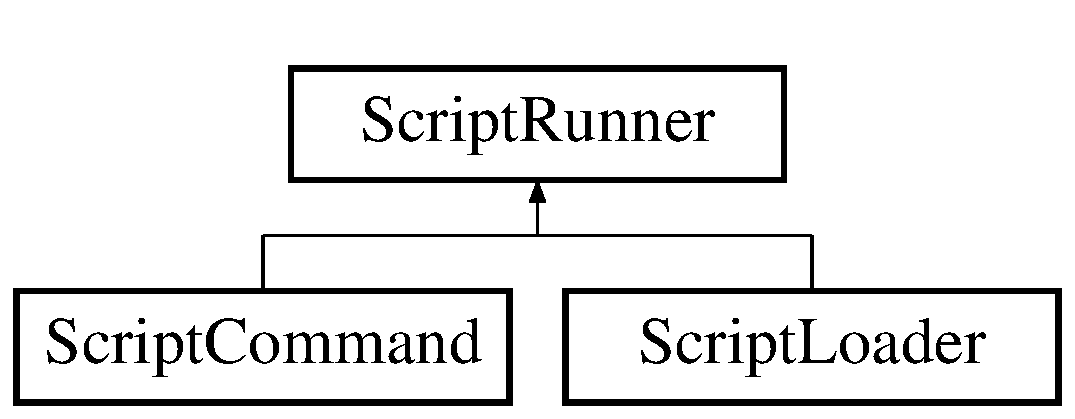
\includegraphics[height=2.000000cm]{class_script_runner}
\end{center}
\end{figure}
\subsection*{Public Member Functions}
\begin{DoxyCompactItemize}
\item 
\hypertarget{class_script_runner_ab4a70a8d8caa68659c42925272e19975}{}virtual void {\bfseries start\+Command} ()=0\label{class_script_runner_ab4a70a8d8caa68659c42925272e19975}

\end{DoxyCompactItemize}


\subsection{Detailed Description}
Starts an arbitrary command. 

The documentation for this class was generated from the following file\+:\begin{DoxyCompactItemize}
\item 
Cyclophosphamide/src/\+Commands/\+Autonomous/Scripting.\+h\end{DoxyCompactItemize}

\hypertarget{class_set_down}{}\section{Set\+Down Class Reference}
\label{class_set_down}\index{Set\+Down@{Set\+Down}}
Inheritance diagram for Set\+Down\+:\begin{figure}[H]
\begin{center}
\leavevmode
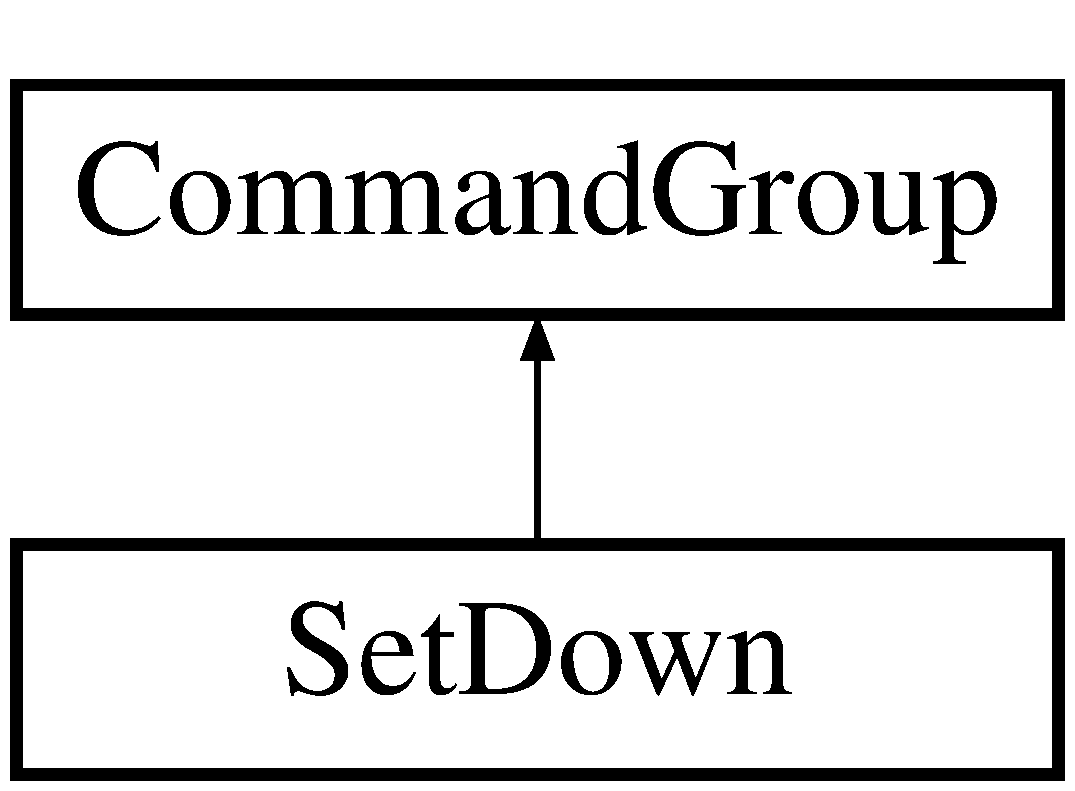
\includegraphics[height=2.000000cm]{class_set_down}
\end{center}
\end{figure}
\subsection*{Public Member Functions}
\begin{DoxyCompactItemize}
\item 
\hyperlink{class_set_down_a928f8a3efd966772da9187cae88a92ad}{Set\+Down} ()
\end{DoxyCompactItemize}


\subsection{Constructor \& Destructor Documentation}
\hypertarget{class_set_down_a928f8a3efd966772da9187cae88a92ad}{}\index{Set\+Down@{Set\+Down}!Set\+Down@{Set\+Down}}
\index{Set\+Down@{Set\+Down}!Set\+Down@{Set\+Down}}
\subsubsection[{Set\+Down}]{\setlength{\rightskip}{0pt plus 5cm}Set\+Down\+::\+Set\+Down (
\begin{DoxyParamCaption}
{}
\end{DoxyParamCaption}
)}\label{class_set_down_a928f8a3efd966772da9187cae88a92ad}
Sets the arms of the cancollecterino to a horizontal position 

The documentation for this class was generated from the following file\+:\begin{DoxyCompactItemize}
\item 
Cyclophosphamide/src/\+Commands/\+Can\+Collecterino/Set\+Down.\+h\end{DoxyCompactItemize}

\hypertarget{class_simple_drive_forward}{}\section{Simple\+Drive\+Forward Class Reference}
\label{class_simple_drive_forward}\index{Simple\+Drive\+Forward@{Simple\+Drive\+Forward}}
Inheritance diagram for Simple\+Drive\+Forward\+:\begin{figure}[H]
\begin{center}
\leavevmode
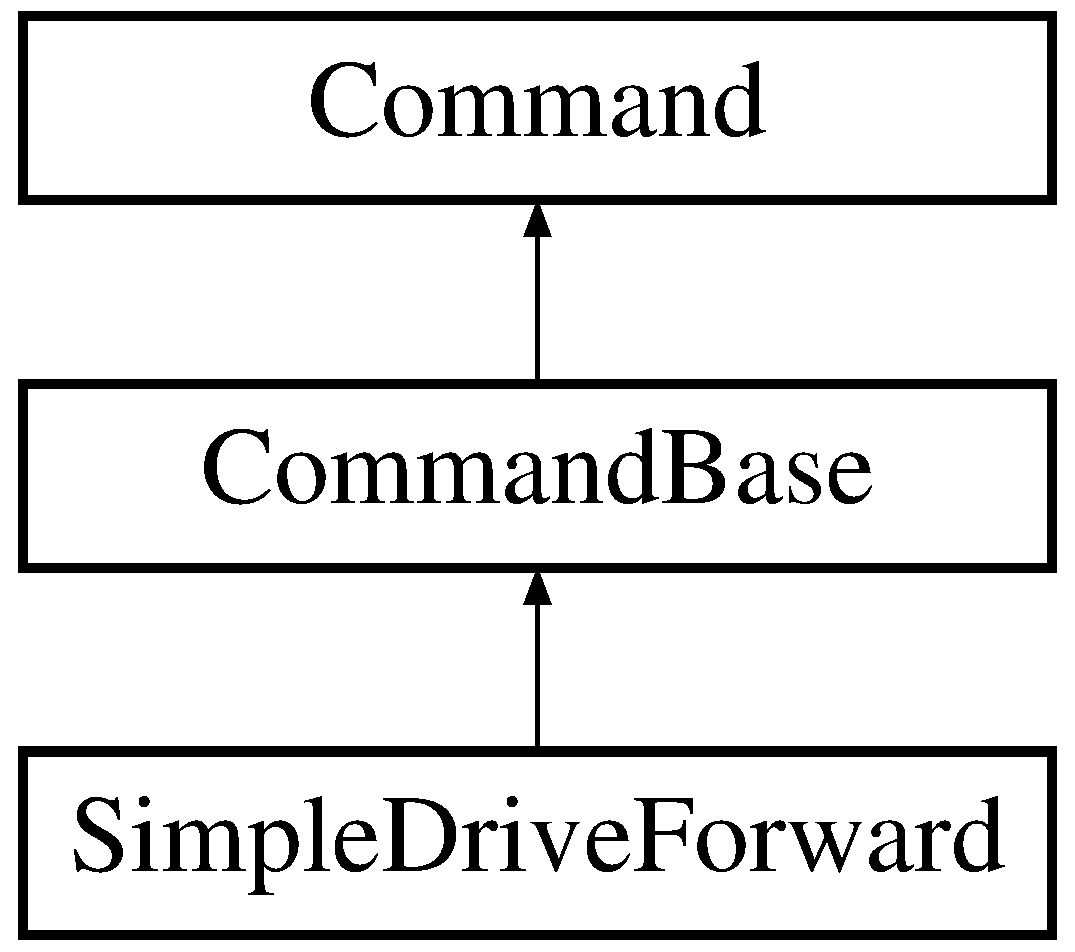
\includegraphics[height=3.000000cm]{class_simple_drive_forward}
\end{center}
\end{figure}
\subsection*{Public Member Functions}
\begin{DoxyCompactItemize}
\item 
\hypertarget{class_simple_drive_forward_a353c4a8d47bc147f7ac3b38185285ede}{}{\bfseries Simple\+Drive\+Forward} (float target, double speed)\label{class_simple_drive_forward_a353c4a8d47bc147f7ac3b38185285ede}

\item 
void \hyperlink{class_simple_drive_forward_a7735d50a6fb897e7ed3a8d67ce5c94b1}{Initialize} ()
\item 
\hypertarget{class_simple_drive_forward_a4e7639c1b9ae203bfb7e1503ff5c844f}{}void {\bfseries Execute} ()\label{class_simple_drive_forward_a4e7639c1b9ae203bfb7e1503ff5c844f}

\item 
\hypertarget{class_simple_drive_forward_a0ec912296de959f11018bdaf5c601279}{}bool {\bfseries Is\+Finished} ()\label{class_simple_drive_forward_a0ec912296de959f11018bdaf5c601279}

\item 
\hypertarget{class_simple_drive_forward_a84d83725f3f380f3b1e7f38fd1f2eeb7}{}void {\bfseries End} ()\label{class_simple_drive_forward_a84d83725f3f380f3b1e7f38fd1f2eeb7}

\item 
\hypertarget{class_simple_drive_forward_a7fe9963981143ec53dc96949b34c6acc}{}void {\bfseries Interrupted} ()\label{class_simple_drive_forward_a7fe9963981143ec53dc96949b34c6acc}

\end{DoxyCompactItemize}
\subsection*{Additional Inherited Members}


\subsection{Member Function Documentation}
\hypertarget{class_simple_drive_forward_a7735d50a6fb897e7ed3a8d67ce5c94b1}{}\index{Simple\+Drive\+Forward@{Simple\+Drive\+Forward}!Initialize@{Initialize}}
\index{Initialize@{Initialize}!Simple\+Drive\+Forward@{Simple\+Drive\+Forward}}
\subsubsection[{Initialize}]{\setlength{\rightskip}{0pt plus 5cm}void Simple\+Drive\+Forward\+::\+Initialize (
\begin{DoxyParamCaption}
{}
\end{DoxyParamCaption}
)}\label{class_simple_drive_forward_a7735d50a6fb897e7ed3a8d67ce5c94b1}
drive\+Bae-\/$>$set\+Speed(speed, speed, speed, speed); 

The documentation for this class was generated from the following files\+:\begin{DoxyCompactItemize}
\item 
Cyclophosphamide/src/\+Commands/\+Automatic/Simple\+Drive\+Forward.\+h\item 
Cyclophosphamide/src/\+Commands/\+Automatic/Simple\+Drive\+Forward.\+cpp\end{DoxyCompactItemize}

\hypertarget{class_stack_pusher}{}\section{Stack\+Pusher Class Reference}
\label{class_stack_pusher}\index{Stack\+Pusher@{Stack\+Pusher}}


{\ttfamily \#include $<$Stack\+Pusher.\+h$>$}

Inheritance diagram for Stack\+Pusher\+:\begin{figure}[H]
\begin{center}
\leavevmode
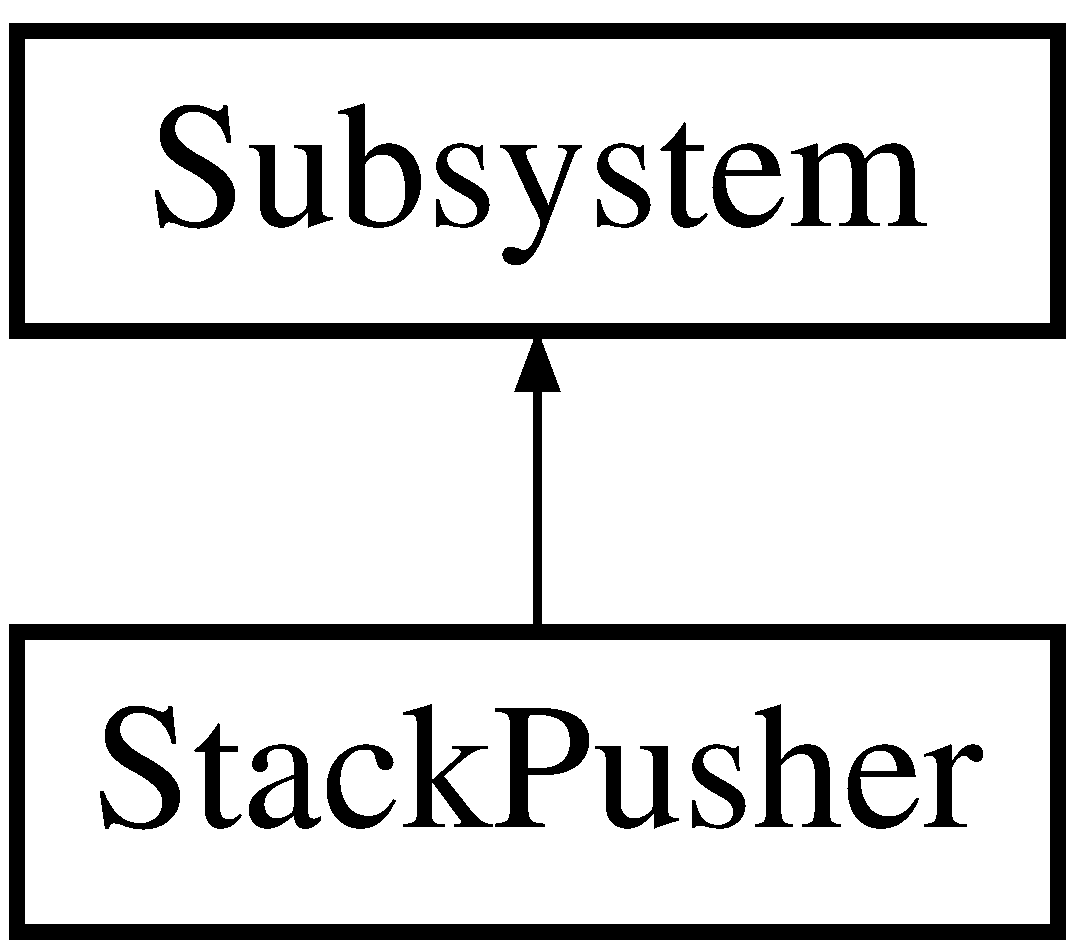
\includegraphics[height=2.000000cm]{class_stack_pusher}
\end{center}
\end{figure}
\subsection*{Public Types}
\begin{DoxyCompactItemize}
\item 
\hypertarget{class_stack_pusher_a0ceaed23d26945569ce1ba0f7a0ac03c}{}enum {\bfseries Push\+State} \{ \\*
{\bfseries push} = true, 
{\bfseries pull} = false, 
{\bfseries toggle}, 
{\bfseries push} = true, 
\\*
{\bfseries pull} = false
 \}\label{class_stack_pusher_a0ceaed23d26945569ce1ba0f7a0ac03c}

\item 
\hypertarget{class_stack_pusher_a0ceaed23d26945569ce1ba0f7a0ac03c}{}enum {\bfseries Push\+State} \{ \\*
{\bfseries push} = true, 
{\bfseries pull} = false, 
{\bfseries toggle}, 
{\bfseries push} = true, 
\\*
{\bfseries pull} = false
 \}\label{class_stack_pusher_a0ceaed23d26945569ce1ba0f7a0ac03c}

\end{DoxyCompactItemize}
\subsection*{Public Member Functions}
\begin{DoxyCompactItemize}
\item 
\hypertarget{class_stack_pusher_ab417d768ab7a62abb345f90f430db33b}{}void {\bfseries Init\+Default\+Command} ()\label{class_stack_pusher_ab417d768ab7a62abb345f90f430db33b}

\item 
\hypertarget{class_stack_pusher_a4483faf60977aee62e81fec2633cd235}{}void {\bfseries Push} ()\label{class_stack_pusher_a4483faf60977aee62e81fec2633cd235}

\item 
\hypertarget{class_stack_pusher_aaf80b44d7b297119070fc5ebd200f66e}{}void {\bfseries Pull} ()\label{class_stack_pusher_aaf80b44d7b297119070fc5ebd200f66e}

\item 
\hypertarget{class_stack_pusher_a282863dc7c3e1cc8d22f5d2fa7e13a05}{}Double\+Solenoid\+::\+Value {\bfseries get\+Value} ()\label{class_stack_pusher_a282863dc7c3e1cc8d22f5d2fa7e13a05}

\item 
\hypertarget{class_stack_pusher_a4bd59d38a910b52c9be86521f57fd3ec}{}Push\+State {\bfseries get\+State} ()\label{class_stack_pusher_a4bd59d38a910b52c9be86521f57fd3ec}

\item 
\hypertarget{class_stack_pusher_ab417d768ab7a62abb345f90f430db33b}{}void {\bfseries Init\+Default\+Command} ()\label{class_stack_pusher_ab417d768ab7a62abb345f90f430db33b}

\item 
\hypertarget{class_stack_pusher_a4483faf60977aee62e81fec2633cd235}{}void {\bfseries Push} ()\label{class_stack_pusher_a4483faf60977aee62e81fec2633cd235}

\item 
\hypertarget{class_stack_pusher_aaf80b44d7b297119070fc5ebd200f66e}{}void {\bfseries Pull} ()\label{class_stack_pusher_aaf80b44d7b297119070fc5ebd200f66e}

\end{DoxyCompactItemize}


\subsection{Detailed Description}
pneumatics Stack Pusher pull in, or push out using the stick that hold to the totes to unload totes. 

The documentation for this class was generated from the following files\+:\begin{DoxyCompactItemize}
\item 
Cyclophosphamide/src/\+Subsystems/Stack\+Pusher.\+h\item 
Cyclophosphamide/src/\+Subsystems/Stack\+Pusher.\+cpp\end{DoxyCompactItemize}

\hypertarget{class_stallable_motor}{}\section{Stallable\+Motor Class Reference}
\label{class_stallable_motor}\index{Stallable\+Motor@{Stallable\+Motor}}
Inheritance diagram for Stallable\+Motor\+:\begin{figure}[H]
\begin{center}
\leavevmode
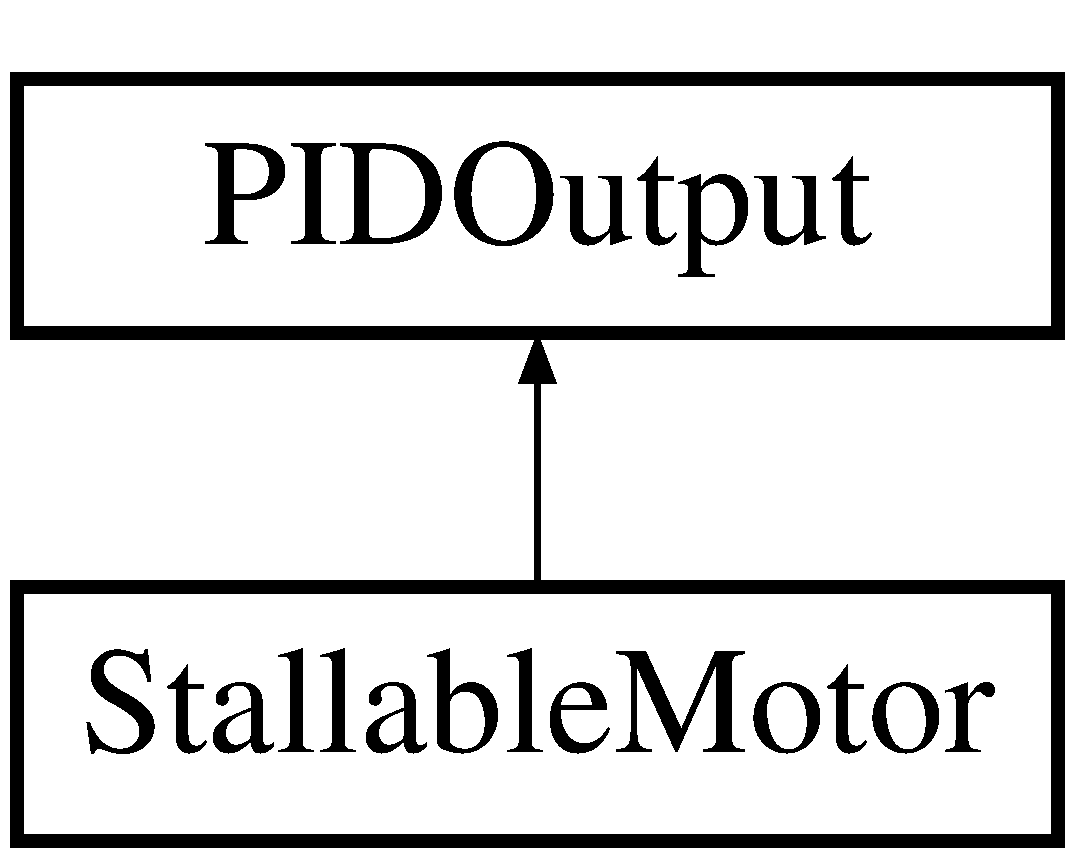
\includegraphics[height=2.000000cm]{class_stallable_motor}
\end{center}
\end{figure}
\subsection*{Public Member Functions}
\begin{DoxyCompactItemize}
\item 
\hypertarget{class_stallable_motor_a5f9ae029cba417b1490e51e6a3498314}{}{\bfseries Stallable\+Motor} (P\+I\+D\+Source $\ast$input, float current\+Threshold, C\+A\+N\+Talon $\ast$motor, C\+A\+N\+Talon $\ast$slave\+Motor=N\+U\+L\+L)\label{class_stallable_motor_a5f9ae029cba417b1490e51e6a3498314}

\item 
\hypertarget{class_stallable_motor_a8e2d132e0a26ee8743a764fbc1c9700c}{}{\bfseries Stallable\+Motor} (C\+A\+N\+Talon $\ast$motor, float current\+Threshold)\label{class_stallable_motor_a8e2d132e0a26ee8743a764fbc1c9700c}

\item 
\hypertarget{class_stallable_motor_aaeab6d6a90993d56431ad2d4033e6eca}{}void {\bfseries Thread\+Kill} ()\label{class_stallable_motor_aaeab6d6a90993d56431ad2d4033e6eca}

\item 
\hypertarget{class_stallable_motor_a0931fab904d5651b2f822b2250552dde}{}void {\bfseries P\+I\+D\+Write} (float output)\label{class_stallable_motor_a0931fab904d5651b2f822b2250552dde}

\end{DoxyCompactItemize}


The documentation for this class was generated from the following files\+:\begin{DoxyCompactItemize}
\item 
Cyclophosphamide/src/utilities/Stallable\+Motor.\+h\item 
Cyclophosphamide/src/utilities/Stallable\+Motor.\+cpp\end{DoxyCompactItemize}

\hypertarget{class_timed_drive}{}\section{Timed\+Drive Class Reference}
\label{class_timed_drive}\index{Timed\+Drive@{Timed\+Drive}}
Inheritance diagram for Timed\+Drive\+:\begin{figure}[H]
\begin{center}
\leavevmode
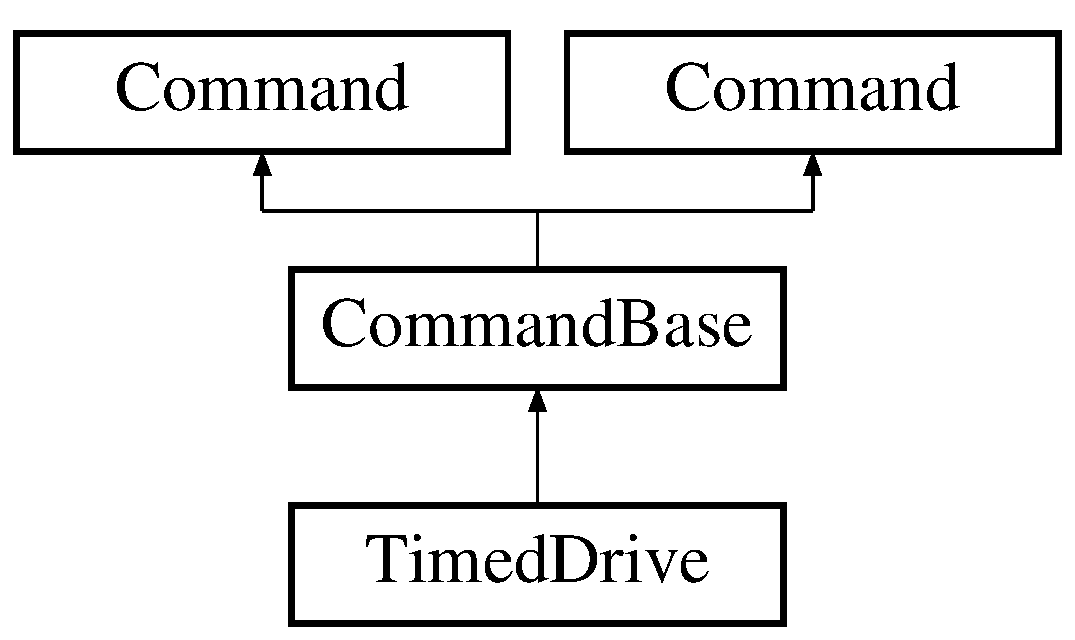
\includegraphics[height=3.000000cm]{class_timed_drive}
\end{center}
\end{figure}
\subsection*{Public Member Functions}
\begin{DoxyCompactItemize}
\item 
\hypertarget{class_timed_drive_a056192c806f771b28d1059b6a32426a0}{}{\bfseries Timed\+Drive} (float duration, float heading)\label{class_timed_drive_a056192c806f771b28d1059b6a32426a0}

\item 
\hypertarget{class_timed_drive_ab7f07fe627966c0b53e3b4b627e476a1}{}void {\bfseries Initialize} ()\label{class_timed_drive_ab7f07fe627966c0b53e3b4b627e476a1}

\item 
\hypertarget{class_timed_drive_adede6a8f93c102aaff6335c7a470028a}{}void {\bfseries Execute} ()\label{class_timed_drive_adede6a8f93c102aaff6335c7a470028a}

\item 
\hypertarget{class_timed_drive_a1b06b3bce24a28d879f927502745dc1a}{}bool {\bfseries Is\+Finished} ()\label{class_timed_drive_a1b06b3bce24a28d879f927502745dc1a}

\item 
\hypertarget{class_timed_drive_a8178e8a9c7f372c9f17276e8279fba92}{}void {\bfseries End} ()\label{class_timed_drive_a8178e8a9c7f372c9f17276e8279fba92}

\item 
\hypertarget{class_timed_drive_af74f16cab8a8081a0940b5bd7566a99e}{}void {\bfseries Interrupted} ()\label{class_timed_drive_af74f16cab8a8081a0940b5bd7566a99e}

\end{DoxyCompactItemize}
\subsection*{Additional Inherited Members}


The documentation for this class was generated from the following files\+:\begin{DoxyCompactItemize}
\item 
Cyclophosphamide/src/\+Commands/\+Automatic/Timed\+Drive.\+h\item 
Cyclophosphamide/src/\+Commands/\+Automatic/Timed\+Drive.\+cpp\end{DoxyCompactItemize}

\hypertarget{class_tote_intake}{}\section{Tote\+Intake Class Reference}
\label{class_tote_intake}\index{Tote\+Intake@{Tote\+Intake}}
Inheritance diagram for Tote\+Intake\+:\begin{figure}[H]
\begin{center}
\leavevmode
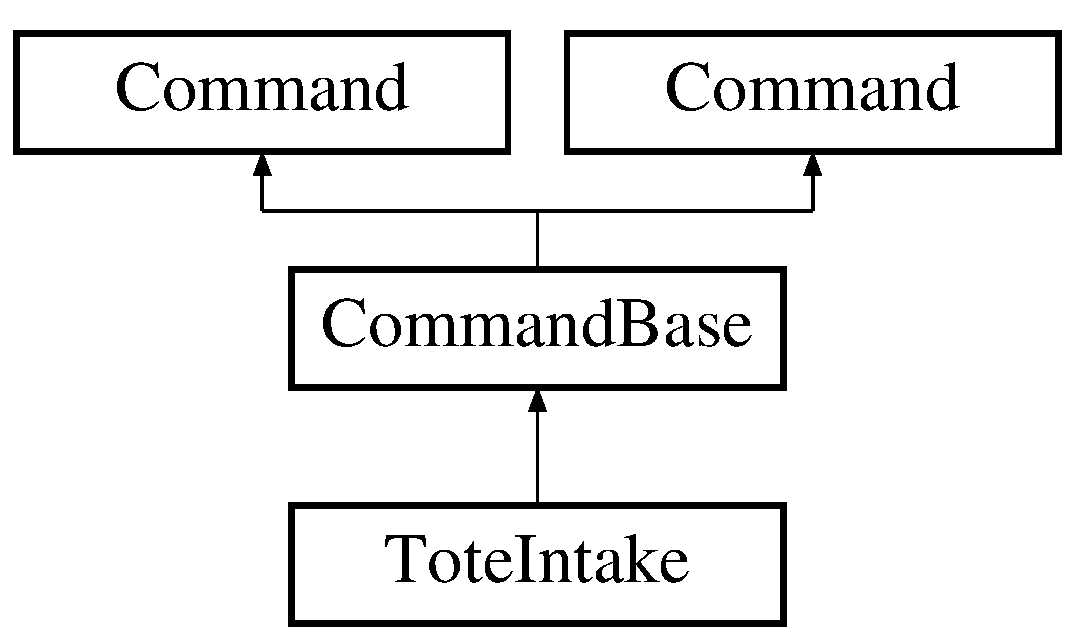
\includegraphics[height=3.000000cm]{class_tote_intake}
\end{center}
\end{figure}
\subsection*{Public Types}
\begin{DoxyCompactItemize}
\item 
\hypertarget{class_tote_intake_a526041a98825e90d7d0db04bf2ad3154}{}enum {\bfseries Direction} \{ {\bfseries forward}, 
{\bfseries reverse}, 
{\bfseries stopped}
 \}\label{class_tote_intake_a526041a98825e90d7d0db04bf2ad3154}

\end{DoxyCompactItemize}
\subsection*{Public Member Functions}
\begin{DoxyCompactItemize}
\item 
\hypertarget{class_tote_intake_ab16b0556811e80666c33603406270ff7}{}{\bfseries Tote\+Intake} (Direction direction)\label{class_tote_intake_ab16b0556811e80666c33603406270ff7}

\item 
\hypertarget{class_tote_intake_a827598afdc7b43772bce4964e86388b3}{}void {\bfseries Initialize} ()\label{class_tote_intake_a827598afdc7b43772bce4964e86388b3}

\item 
\hypertarget{class_tote_intake_a034514f1dc307f9e7d609403496931b0}{}void {\bfseries Execute} ()\label{class_tote_intake_a034514f1dc307f9e7d609403496931b0}

\item 
\hypertarget{class_tote_intake_af56496899456386ddd5a1396ceaa44e2}{}bool {\bfseries Is\+Finished} ()\label{class_tote_intake_af56496899456386ddd5a1396ceaa44e2}

\item 
\hypertarget{class_tote_intake_a1e801691281940bcc410dfcd1a3f13ac}{}void {\bfseries End} ()\label{class_tote_intake_a1e801691281940bcc410dfcd1a3f13ac}

\item 
\hypertarget{class_tote_intake_a08d4690348e422e6dfedcff4758edaf7}{}void {\bfseries Interrupted} ()\label{class_tote_intake_a08d4690348e422e6dfedcff4758edaf7}

\end{DoxyCompactItemize}
\subsection*{Additional Inherited Members}


The documentation for this class was generated from the following files\+:\begin{DoxyCompactItemize}
\item 
Cyclophosphamide/src/\+Commands/\+Tote\+Handling/Tote\+Intake.\+h\item 
Cyclophosphamide/src/\+Commands/\+Tote\+Handling/Tote\+Intake.\+cpp\end{DoxyCompactItemize}

\hypertarget{class_tote_intakerino}{}\section{Tote\+Intakerino Class Reference}
\label{class_tote_intakerino}\index{Tote\+Intakerino@{Tote\+Intakerino}}


{\ttfamily \#include $<$Tote\+Intakerino.\+h$>$}

Inheritance diagram for Tote\+Intakerino\+:\begin{figure}[H]
\begin{center}
\leavevmode
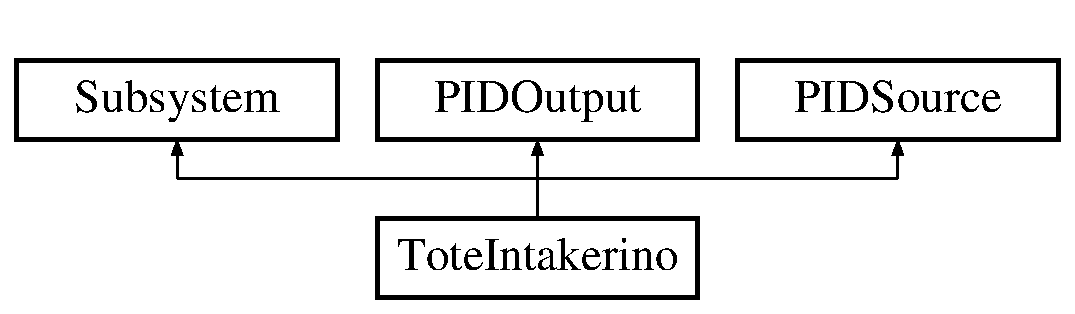
\includegraphics[height=2.000000cm]{class_tote_intakerino}
\end{center}
\end{figure}
\subsection*{Public Member Functions}
\begin{DoxyCompactItemize}
\item 
\hyperlink{class_tote_intakerino_a754194267a81d64543ca83d0ca0b6846}{Tote\+Intakerino} ()
\item 
void \hyperlink{class_tote_intakerino_a57cd7612442d6a91f12e4e736f6f9715}{Init\+Default\+Command} ()
\item 
void \hyperlink{class_tote_intakerino_a638941b4ab78e4012e7e2c3061e121e0}{set\+Motor} (float speed)
\item 
void \hyperlink{class_tote_intakerino_a2edb12308d1b27cb5a07e7bd01c1a889}{hold} ()
\item 
bool \hyperlink{class_tote_intakerino_a8c225c0792fddce3e79f07a0faad1318}{is\+Loaded} ()
\item 
\hypertarget{class_tote_intakerino_aaed3645ed0174f77bc542e5650019411}{}Encoder $\ast$ {\bfseries get\+Encoder} ()\label{class_tote_intakerino_aaed3645ed0174f77bc542e5650019411}

\item 
\hypertarget{class_tote_intakerino_a746600f1fd998f1bf686c711bc7d31a5}{}virtual void {\bfseries P\+I\+D\+Write} (float f)\label{class_tote_intakerino_a746600f1fd998f1bf686c711bc7d31a5}

\item 
\hypertarget{class_tote_intakerino_a3045993c8702f1b8bd5827090da1f1ad}{}virtual double {\bfseries P\+I\+D\+Get} ()\label{class_tote_intakerino_a3045993c8702f1b8bd5827090da1f1ad}

\end{DoxyCompactItemize}


\subsection{Detailed Description}
Subsystem for loading totes from the human loader station encoders runs off/on P\+I\+D setpoint 0 (ground level) 

\subsection{Constructor \& Destructor Documentation}
\hypertarget{class_tote_intakerino_a754194267a81d64543ca83d0ca0b6846}{}\index{Tote\+Intakerino@{Tote\+Intakerino}!Tote\+Intakerino@{Tote\+Intakerino}}
\index{Tote\+Intakerino@{Tote\+Intakerino}!Tote\+Intakerino@{Tote\+Intakerino}}
\subsubsection[{Tote\+Intakerino}]{\setlength{\rightskip}{0pt plus 5cm}Tote\+Intakerino\+::\+Tote\+Intakerino (
\begin{DoxyParamCaption}
{}
\end{DoxyParamCaption}
)}\label{class_tote_intakerino_a754194267a81d64543ca83d0ca0b6846}
Default constructor 

\subsection{Member Function Documentation}
\hypertarget{class_tote_intakerino_a2edb12308d1b27cb5a07e7bd01c1a889}{}\index{Tote\+Intakerino@{Tote\+Intakerino}!hold@{hold}}
\index{hold@{hold}!Tote\+Intakerino@{Tote\+Intakerino}}
\subsubsection[{hold}]{\setlength{\rightskip}{0pt plus 5cm}void Tote\+Intakerino\+::hold (
\begin{DoxyParamCaption}
{}
\end{DoxyParamCaption}
)}\label{class_tote_intakerino_a2edb12308d1b27cb5a07e7bd01c1a889}
Stop the motors and keeps them at their current position \hypertarget{class_tote_intakerino_a57cd7612442d6a91f12e4e736f6f9715}{}\index{Tote\+Intakerino@{Tote\+Intakerino}!Init\+Default\+Command@{Init\+Default\+Command}}
\index{Init\+Default\+Command@{Init\+Default\+Command}!Tote\+Intakerino@{Tote\+Intakerino}}
\subsubsection[{Init\+Default\+Command}]{\setlength{\rightskip}{0pt plus 5cm}void Tote\+Intakerino\+::\+Init\+Default\+Command (
\begin{DoxyParamCaption}
{}
\end{DoxyParamCaption}
)}\label{class_tote_intakerino_a57cd7612442d6a91f12e4e736f6f9715}
Does nothing because call creates circular dependencies and compile errors \hypertarget{class_tote_intakerino_a8c225c0792fddce3e79f07a0faad1318}{}\index{Tote\+Intakerino@{Tote\+Intakerino}!is\+Loaded@{is\+Loaded}}
\index{is\+Loaded@{is\+Loaded}!Tote\+Intakerino@{Tote\+Intakerino}}
\subsubsection[{is\+Loaded}]{\setlength{\rightskip}{0pt plus 5cm}bool Tote\+Intakerino\+::is\+Loaded (
\begin{DoxyParamCaption}
{}
\end{DoxyParamCaption}
)}\label{class_tote_intakerino_a8c225c0792fddce3e79f07a0faad1318}
Tells if a tote is loaded based on the work done by the P\+I\+D \hypertarget{class_tote_intakerino_a638941b4ab78e4012e7e2c3061e121e0}{}\index{Tote\+Intakerino@{Tote\+Intakerino}!set\+Motor@{set\+Motor}}
\index{set\+Motor@{set\+Motor}!Tote\+Intakerino@{Tote\+Intakerino}}
\subsubsection[{set\+Motor}]{\setlength{\rightskip}{0pt plus 5cm}void Tote\+Intakerino\+::set\+Motor (
\begin{DoxyParamCaption}
\item[{float}]{speed}
\end{DoxyParamCaption}
)}\label{class_tote_intakerino_a638941b4ab78e4012e7e2c3061e121e0}
Sets the speed of rollers that pull the tote in 
\begin{DoxyParams}{Parameters}
{\em speed} & value to set the motor to \\
\hline
\end{DoxyParams}


The documentation for this class was generated from the following files\+:\begin{DoxyCompactItemize}
\item 
Cyclophosphamide/src/\+Subsystems/Tote\+Intakerino.\+h\item 
Cyclophosphamide/src/\+Subsystems/Tote\+Intakerino.\+cpp\end{DoxyCompactItemize}

\hypertarget{class_tote_lifterino}{}\section{Tote\+Lifterino Class Reference}
\label{class_tote_lifterino}\index{Tote\+Lifterino@{Tote\+Lifterino}}


{\ttfamily \#include $<$Tote\+Lifterino.\+h$>$}

Inheritance diagram for Tote\+Lifterino\+:\begin{figure}[H]
\begin{center}
\leavevmode
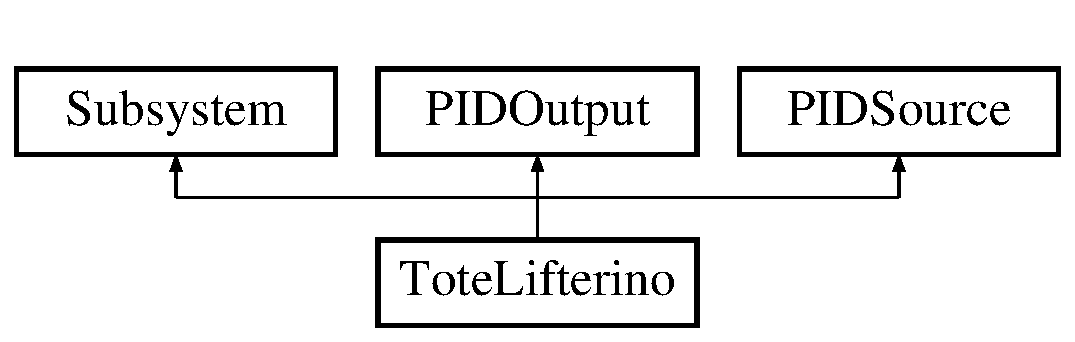
\includegraphics[height=2.000000cm]{class_tote_lifterino}
\end{center}
\end{figure}
\subsection*{Public Member Functions}
\begin{DoxyCompactItemize}
\item 
\hypertarget{class_tote_lifterino_a972bde0b7cb90474cf63fadad3a9297c}{}void {\bfseries Init\+Default\+Command} ()\label{class_tote_lifterino_a972bde0b7cb90474cf63fadad3a9297c}

\item 
\hypertarget{class_tote_lifterino_a7f0063d9a14e6a9413e7b38847854962}{}bool {\bfseries get\+Mag\+Input} ()\label{class_tote_lifterino_a7f0063d9a14e6a9413e7b38847854962}

\item 
\hypertarget{class_tote_lifterino_a039877dfaec2b0bc1c722ac852674b78}{}void {\bfseries set\+Zeroed} (bool zeroed)\label{class_tote_lifterino_a039877dfaec2b0bc1c722ac852674b78}

\item 
\hypertarget{class_tote_lifterino_a3a5cbfd809e851a8cbd5202ea0565626}{}bool {\bfseries lower\+Than} (double height)\label{class_tote_lifterino_a3a5cbfd809e851a8cbd5202ea0565626}

\item 
\hypertarget{class_tote_lifterino_a853d0d90d50406b572d1518719e4f866}{}C\+A\+N\+Talon $\ast$ {\bfseries get\+Left\+Motor} ()\label{class_tote_lifterino_a853d0d90d50406b572d1518719e4f866}

\item 
\hypertarget{class_tote_lifterino_abda31d2e071bd526afd95a35d7dc0f14}{}C\+A\+N\+Talon $\ast$ {\bfseries get\+Right\+Motor} ()\label{class_tote_lifterino_abda31d2e071bd526afd95a35d7dc0f14}

\item 
\hypertarget{class_tote_lifterino_a2bf754226a84928655ad00a1fa5dc7a6}{}double {\bfseries get\+Position} ()\label{class_tote_lifterino_a2bf754226a84928655ad00a1fa5dc7a6}

\item 
\hypertarget{class_tote_lifterino_a2e7f3a02eebaddca1805c282715a6659}{}Encoder $\ast$ {\bfseries get\+Encoder} ()\label{class_tote_lifterino_a2e7f3a02eebaddca1805c282715a6659}

\item 
\hypertarget{class_tote_lifterino_af6781e4b7e6a9a5e1f7f8e68ff84500c}{}P\+I\+D\+Controller $\ast$ {\bfseries get\+P\+I\+D} ()\label{class_tote_lifterino_af6781e4b7e6a9a5e1f7f8e68ff84500c}

\item 
\hypertarget{class_tote_lifterino_a6d449a8d4da13035d3f8e0088800f17e}{}bool {\bfseries close\+Enough} (float destination)\label{class_tote_lifterino_a6d449a8d4da13035d3f8e0088800f17e}

\item 
\hypertarget{class_tote_lifterino_a116242e1863680c49bc06d4b1156fa3a}{}void {\bfseries set\+Motor\+Speed} (double speed)\label{class_tote_lifterino_a116242e1863680c49bc06d4b1156fa3a}

\item 
\hypertarget{class_tote_lifterino_a250fddcbc35ffcb892d2f5575f6ebf4c}{}void {\bfseries set\+Set\+Points} (double set\+Point)\label{class_tote_lifterino_a250fddcbc35ffcb892d2f5575f6ebf4c}

\item 
\hypertarget{class_tote_lifterino_a8c56fb38fc532d99435c45eb500f78a7}{}void {\bfseries enable\+P\+I\+D} (bool enable)\label{class_tote_lifterino_a8c56fb38fc532d99435c45eb500f78a7}

\item 
\hypertarget{class_tote_lifterino_a4052d75b1f14d29faab681e93e41ac3c}{}virtual void {\bfseries P\+I\+D\+Write} (float f)\label{class_tote_lifterino_a4052d75b1f14d29faab681e93e41ac3c}

\item 
\hypertarget{class_tote_lifterino_a61ffaaf13e324571879ab8f353e8cd9d}{}virtual double {\bfseries P\+I\+D\+Get} ()\label{class_tote_lifterino_a61ffaaf13e324571879ab8f353e8cd9d}

\end{DoxyCompactItemize}


\subsection{Detailed Description}
Lift or elevate the totes up and down. P\+I\+D have the set point that elevates up/ down with certain height. Encoders 

The documentation for this class was generated from the following files\+:\begin{DoxyCompactItemize}
\item 
Cyclophosphamide/src/\+Subsystems/Tote\+Lifterino.\+h\item 
Cyclophosphamide/src/\+Subsystems/Tote\+Lifterino.\+cpp\end{DoxyCompactItemize}

\hypertarget{class_turn_to}{}\section{Turn\+To Class Reference}
\label{class_turn_to}\index{Turn\+To@{Turn\+To}}
Inheritance diagram for Turn\+To\+:\begin{figure}[H]
\begin{center}
\leavevmode
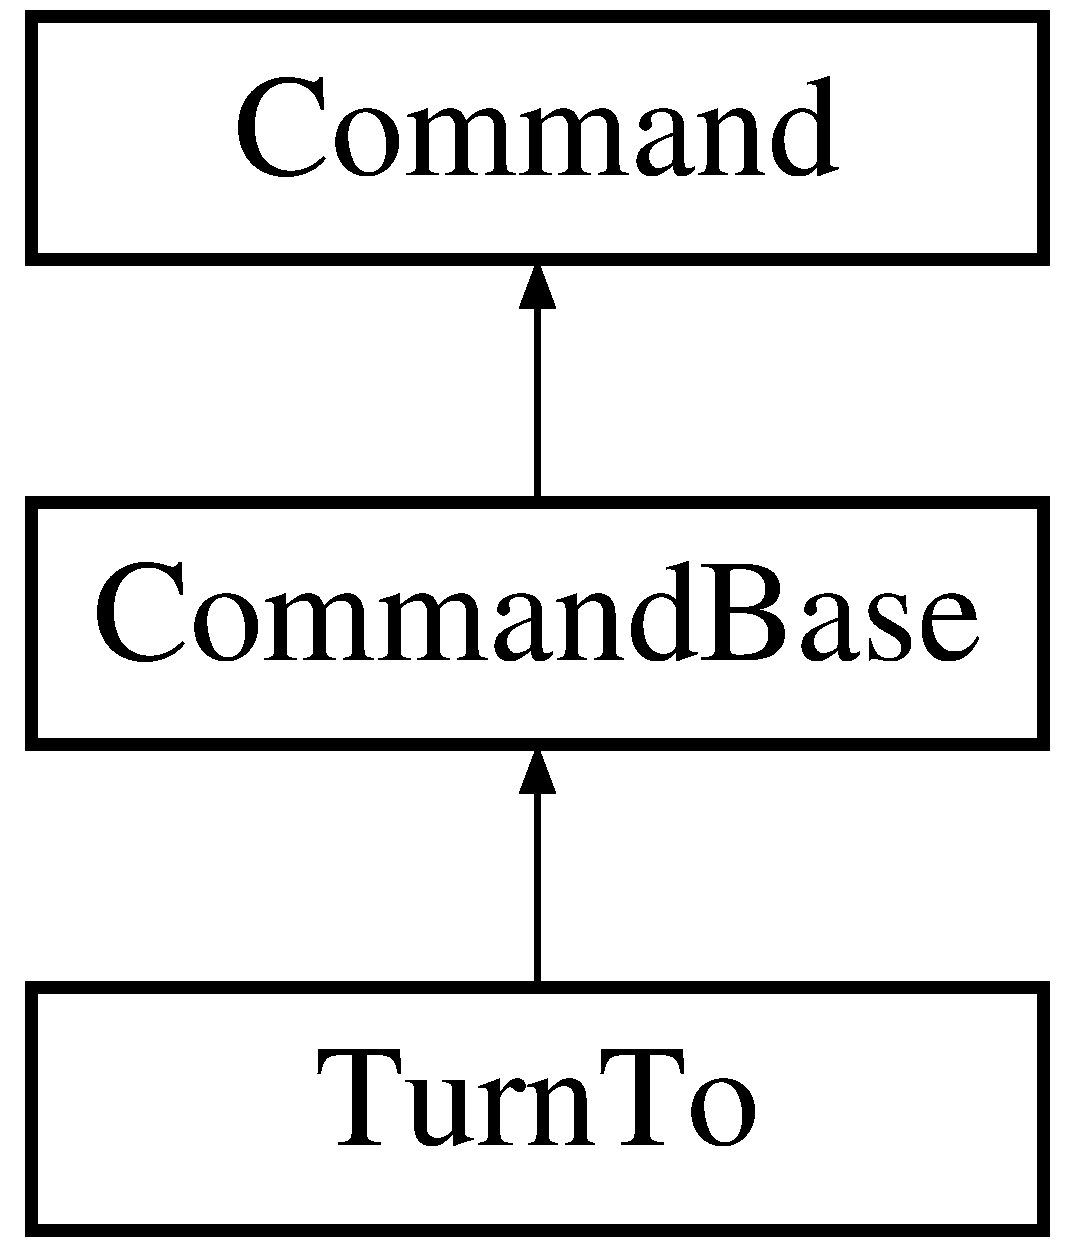
\includegraphics[height=3.000000cm]{class_turn_to}
\end{center}
\end{figure}
\subsection*{Public Member Functions}
\begin{DoxyCompactItemize}
\item 
\hypertarget{class_turn_to_aa74a4bd0785dce24fdda1e1bf79cd39b}{}{\bfseries Turn\+To} (float target\+Angle)\label{class_turn_to_aa74a4bd0785dce24fdda1e1bf79cd39b}

\item 
\hypertarget{class_turn_to_a1573bc8d8345d2dbe40866937d4e41a1}{}void {\bfseries Initialize} ()\label{class_turn_to_a1573bc8d8345d2dbe40866937d4e41a1}

\item 
\hypertarget{class_turn_to_ae60afcdabfc0510abf2718f89919e8df}{}void {\bfseries Execute} ()\label{class_turn_to_ae60afcdabfc0510abf2718f89919e8df}

\item 
\hypertarget{class_turn_to_a645fa93286ea2657ec45166ec9a10662}{}bool {\bfseries Is\+Finished} ()\label{class_turn_to_a645fa93286ea2657ec45166ec9a10662}

\item 
\hypertarget{class_turn_to_a22e332211c9979bc29d408299f5d6188}{}void {\bfseries End} ()\label{class_turn_to_a22e332211c9979bc29d408299f5d6188}

\item 
\hypertarget{class_turn_to_a89e338cc7fd550fb0f2e6fb75698ae05}{}void {\bfseries Interrupted} ()\label{class_turn_to_a89e338cc7fd550fb0f2e6fb75698ae05}

\item 
\hypertarget{class_turn_to_aa74a4bd0785dce24fdda1e1bf79cd39b}{}{\bfseries Turn\+To} (float target\+Angle)\label{class_turn_to_aa74a4bd0785dce24fdda1e1bf79cd39b}

\item 
\hypertarget{class_turn_to_a1573bc8d8345d2dbe40866937d4e41a1}{}void {\bfseries Initialize} ()\label{class_turn_to_a1573bc8d8345d2dbe40866937d4e41a1}

\item 
\hypertarget{class_turn_to_ae60afcdabfc0510abf2718f89919e8df}{}void {\bfseries Execute} ()\label{class_turn_to_ae60afcdabfc0510abf2718f89919e8df}

\item 
\hypertarget{class_turn_to_a645fa93286ea2657ec45166ec9a10662}{}bool {\bfseries Is\+Finished} ()\label{class_turn_to_a645fa93286ea2657ec45166ec9a10662}

\item 
\hypertarget{class_turn_to_a22e332211c9979bc29d408299f5d6188}{}void {\bfseries End} ()\label{class_turn_to_a22e332211c9979bc29d408299f5d6188}

\item 
\hypertarget{class_turn_to_a89e338cc7fd550fb0f2e6fb75698ae05}{}void {\bfseries Interrupted} ()\label{class_turn_to_a89e338cc7fd550fb0f2e6fb75698ae05}

\end{DoxyCompactItemize}
\subsection*{Additional Inherited Members}


The documentation for this class was generated from the following files\+:\begin{DoxyCompactItemize}
\item 
Cyclophosphamide/src/\+Commands/\+Automatic/Turn\+To.\+h\item 
One\+Stick\+Mecanum/src/\+Commands/\+Automatic/Turn\+Degree.\+h\item 
Cyclophosphamide/src/\+Commands/\+Automatic/Turn\+To.\+cpp\item 
One\+Stick\+Mecanum/src/\+Commands/\+Automatic/Turn\+Degree.\+cpp\end{DoxyCompactItemize}

\hypertarget{class_turn_to_then_drive}{}\section{Turn\+To\+Then\+Drive Class Reference}
\label{class_turn_to_then_drive}\index{Turn\+To\+Then\+Drive@{Turn\+To\+Then\+Drive}}
Inheritance diagram for Turn\+To\+Then\+Drive\+:\begin{figure}[H]
\begin{center}
\leavevmode
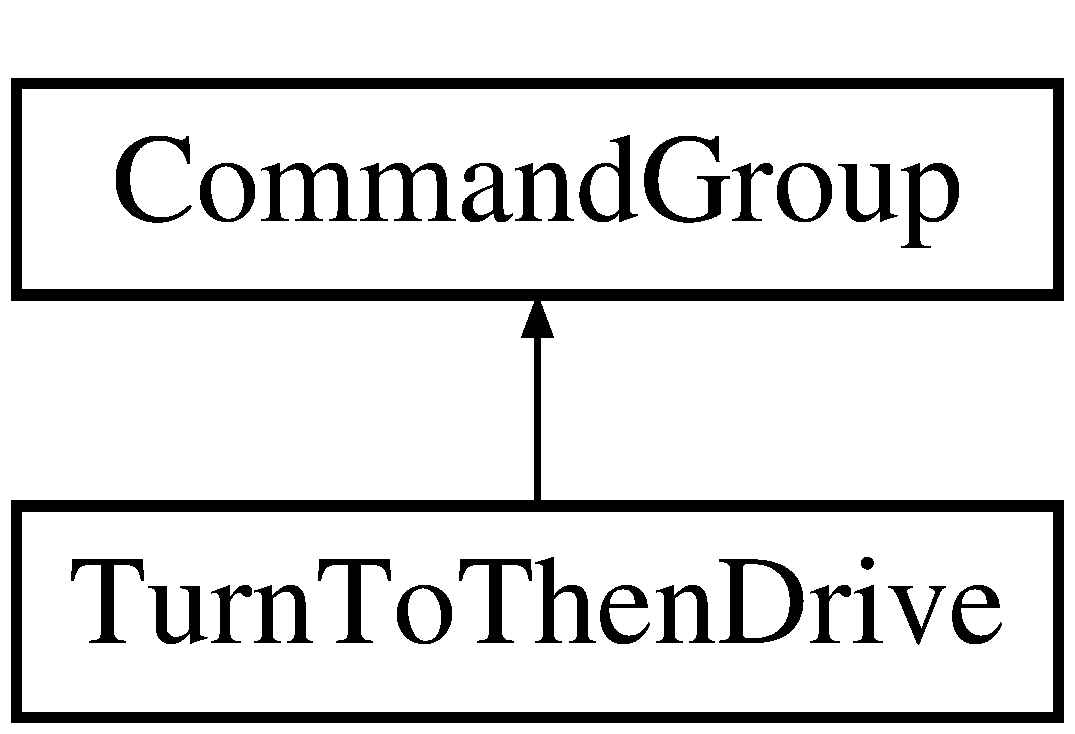
\includegraphics[height=2.000000cm]{class_turn_to_then_drive}
\end{center}
\end{figure}
\subsection*{Public Member Functions}
\begin{DoxyCompactItemize}
\item 
\hypertarget{class_turn_to_then_drive_a827a2f68850522352a7ce5b21c37f76b}{}{\bfseries Turn\+To\+Then\+Drive} (float target\+Angle)\label{class_turn_to_then_drive_a827a2f68850522352a7ce5b21c37f76b}

\end{DoxyCompactItemize}


The documentation for this class was generated from the following files\+:\begin{DoxyCompactItemize}
\item 
Cyclophosphamide/src/\+Commands/\+Automatic/Turn\+To\+Then\+Drive.\+h\item 
Cyclophosphamide/src/\+Commands/\+Automatic/Turn\+To\+Then\+Drive.\+cpp\end{DoxyCompactItemize}

\hypertarget{class_unrustle_gyro}{}\section{Unrustle\+Gyro Class Reference}
\label{class_unrustle_gyro}\index{Unrustle\+Gyro@{Unrustle\+Gyro}}
Inheritance diagram for Unrustle\+Gyro\+:\begin{figure}[H]
\begin{center}
\leavevmode
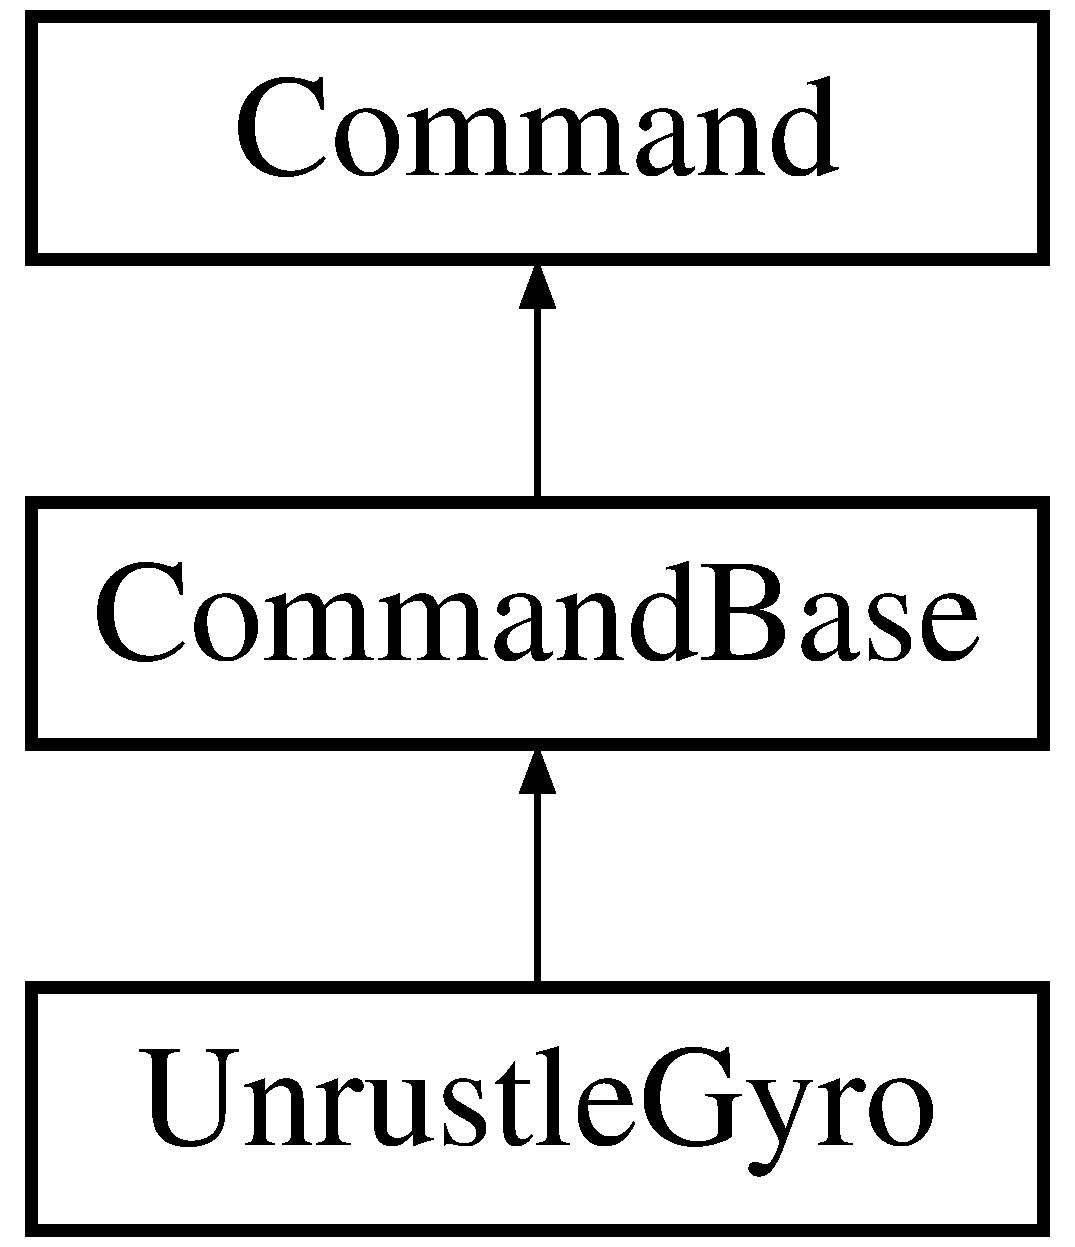
\includegraphics[height=3.000000cm]{class_unrustle_gyro}
\end{center}
\end{figure}
\subsection*{Public Member Functions}
\begin{DoxyCompactItemize}
\item 
\hyperlink{class_unrustle_gyro_a7c6bc39a592510446374913f0e68761f}{Unrustle\+Gyro} ()
\item 
\hypertarget{class_unrustle_gyro_a529fdd89c9702dcbd8f7903065d725b2}{}void {\bfseries Initialize} ()\label{class_unrustle_gyro_a529fdd89c9702dcbd8f7903065d725b2}

\item 
\hypertarget{class_unrustle_gyro_ab72fe5e39db6bc546eaba44c9c667dfc}{}void {\bfseries Execute} ()\label{class_unrustle_gyro_ab72fe5e39db6bc546eaba44c9c667dfc}

\item 
\hypertarget{class_unrustle_gyro_a5a66a724c6e222a7bbd4da6db5575692}{}bool {\bfseries Is\+Finished} ()\label{class_unrustle_gyro_a5a66a724c6e222a7bbd4da6db5575692}

\item 
\hypertarget{class_unrustle_gyro_a9a871544974afb6935826b30bd319d0f}{}void {\bfseries End} ()\label{class_unrustle_gyro_a9a871544974afb6935826b30bd319d0f}

\item 
\hypertarget{class_unrustle_gyro_adf5ab1c63dbca8f1e8705b061d15534d}{}void {\bfseries Interrupted} ()\label{class_unrustle_gyro_adf5ab1c63dbca8f1e8705b061d15534d}

\end{DoxyCompactItemize}
\subsection*{Additional Inherited Members}


\subsection{Constructor \& Destructor Documentation}
\hypertarget{class_unrustle_gyro_a7c6bc39a592510446374913f0e68761f}{}\index{Unrustle\+Gyro@{Unrustle\+Gyro}!Unrustle\+Gyro@{Unrustle\+Gyro}}
\index{Unrustle\+Gyro@{Unrustle\+Gyro}!Unrustle\+Gyro@{Unrustle\+Gyro}}
\subsubsection[{Unrustle\+Gyro}]{\setlength{\rightskip}{0pt plus 5cm}Unrustle\+Gyro\+::\+Unrustle\+Gyro (
\begin{DoxyParamCaption}
{}
\end{DoxyParamCaption}
)}\label{class_unrustle_gyro_a7c6bc39a592510446374913f0e68761f}
Sets the drivebase P\+I\+D to the current position 

The documentation for this class was generated from the following files\+:\begin{DoxyCompactItemize}
\item 
Cyclophosphamide/src/\+Commands/\+Drivebase/Unrustle\+Gyro.\+h\item 
Cyclophosphamide/src/\+Commands/\+Drivebase/Unrustle\+Gyro.\+cpp\end{DoxyCompactItemize}

\hypertarget{class_update_compressor}{}\section{Update\+Compressor Class Reference}
\label{class_update_compressor}\index{Update\+Compressor@{Update\+Compressor}}
Inheritance diagram for Update\+Compressor\+:\begin{figure}[H]
\begin{center}
\leavevmode
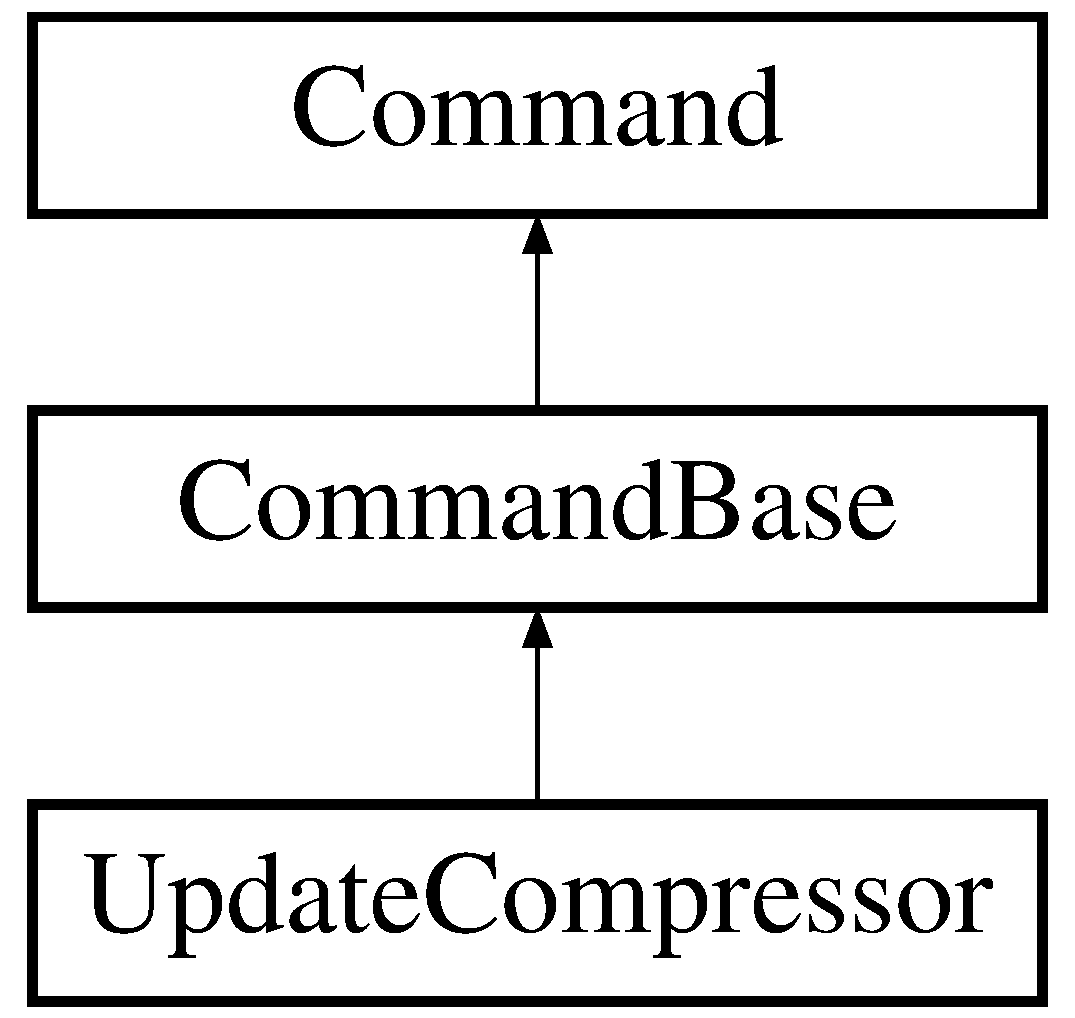
\includegraphics[height=3.000000cm]{class_update_compressor}
\end{center}
\end{figure}
\subsection*{Public Member Functions}
\begin{DoxyCompactItemize}
\item 
\hypertarget{class_update_compressor_aa9b278faa22a0b30d74ba0bf5c283621}{}void {\bfseries Initialize} ()\label{class_update_compressor_aa9b278faa22a0b30d74ba0bf5c283621}

\item 
\hypertarget{class_update_compressor_a1dae416361c23fb33ba08255cf6c5df2}{}void {\bfseries Execute} ()\label{class_update_compressor_a1dae416361c23fb33ba08255cf6c5df2}

\item 
\hypertarget{class_update_compressor_a2a1604f7fff8e360a33f371cd2b9ebb1}{}bool {\bfseries Is\+Finished} ()\label{class_update_compressor_a2a1604f7fff8e360a33f371cd2b9ebb1}

\item 
\hypertarget{class_update_compressor_ac6f4086fde7c7eac4a79cf9b65a58ee5}{}void {\bfseries End} ()\label{class_update_compressor_ac6f4086fde7c7eac4a79cf9b65a58ee5}

\item 
\hypertarget{class_update_compressor_a4fc03700e69bcd8ab2b510e754e9a15d}{}void {\bfseries Interrupted} ()\label{class_update_compressor_a4fc03700e69bcd8ab2b510e754e9a15d}

\item 
\hypertarget{class_update_compressor_aa9b278faa22a0b30d74ba0bf5c283621}{}void {\bfseries Initialize} ()\label{class_update_compressor_aa9b278faa22a0b30d74ba0bf5c283621}

\item 
\hypertarget{class_update_compressor_a1dae416361c23fb33ba08255cf6c5df2}{}void {\bfseries Execute} ()\label{class_update_compressor_a1dae416361c23fb33ba08255cf6c5df2}

\item 
\hypertarget{class_update_compressor_a2a1604f7fff8e360a33f371cd2b9ebb1}{}bool {\bfseries Is\+Finished} ()\label{class_update_compressor_a2a1604f7fff8e360a33f371cd2b9ebb1}

\item 
\hypertarget{class_update_compressor_ac6f4086fde7c7eac4a79cf9b65a58ee5}{}void {\bfseries End} ()\label{class_update_compressor_ac6f4086fde7c7eac4a79cf9b65a58ee5}

\item 
\hypertarget{class_update_compressor_a4fc03700e69bcd8ab2b510e754e9a15d}{}void {\bfseries Interrupted} ()\label{class_update_compressor_a4fc03700e69bcd8ab2b510e754e9a15d}

\end{DoxyCompactItemize}
\subsection*{Additional Inherited Members}


The documentation for this class was generated from the following files\+:\begin{DoxyCompactItemize}
\item 
Cyclophosphamide/src/\+Commands/Update\+Compressor.\+h\item 
Cyclophosphamide/src/\+Commands/Update\+Compressor.\+cpp\end{DoxyCompactItemize}

\hypertarget{class_whack}{}\section{Whack Class Reference}
\label{class_whack}\index{Whack@{Whack}}
Inheritance diagram for Whack\+:\begin{figure}[H]
\begin{center}
\leavevmode
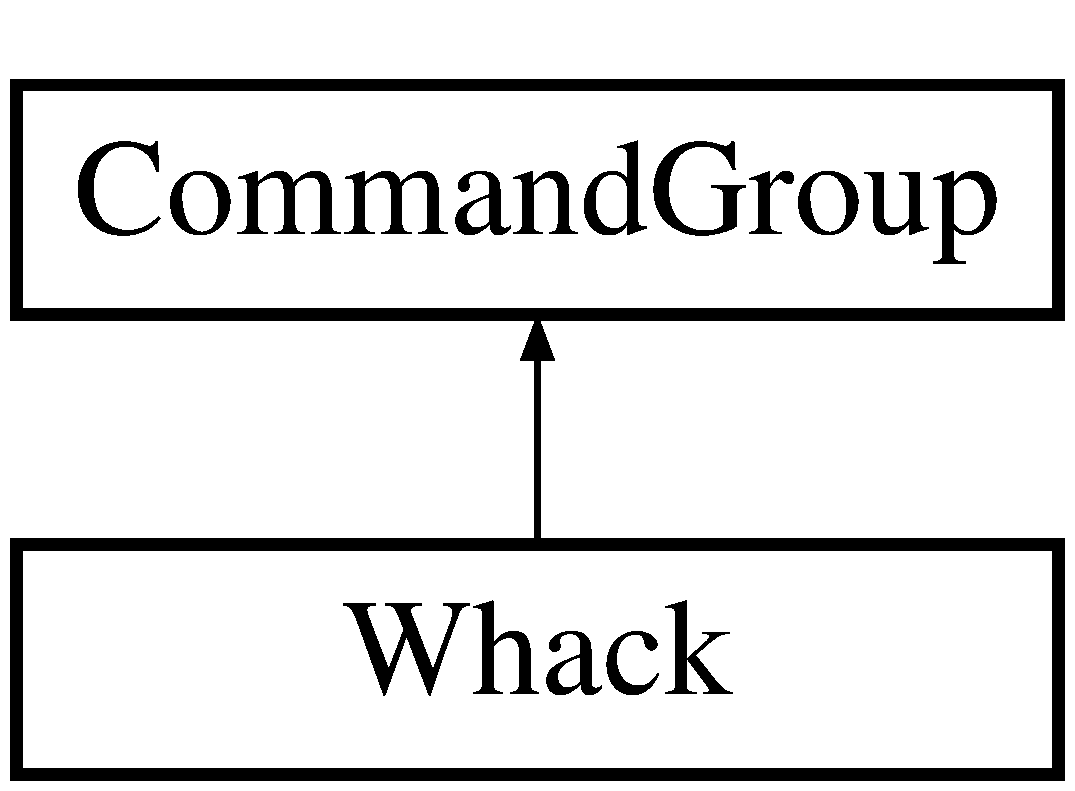
\includegraphics[height=2.000000cm]{class_whack}
\end{center}
\end{figure}
\subsection*{Public Member Functions}
\begin{DoxyCompactItemize}
\item 
\hyperlink{class_whack_a7dba4e263d24cb5239f40c354e406385}{Whack} ()
\end{DoxyCompactItemize}


\subsection{Constructor \& Destructor Documentation}
\hypertarget{class_whack_a7dba4e263d24cb5239f40c354e406385}{}\index{Whack@{Whack}!Whack@{Whack}}
\index{Whack@{Whack}!Whack@{Whack}}
\subsubsection[{Whack}]{\setlength{\rightskip}{0pt plus 5cm}Whack\+::\+Whack (
\begin{DoxyParamCaption}
{}
\end{DoxyParamCaption}
)}\label{class_whack_a7dba4e263d24cb5239f40c354e406385}
Tobacco is whacko if you\textquotesingle{}re a teen 

The documentation for this class was generated from the following files\+:\begin{DoxyCompactItemize}
\item 
Cyclophosphamide/src/\+Commands/\+Can\+Collecterino/\+Arms/Whack.\+h\item 
Cyclophosphamide/src/\+Commands/\+Can\+Collecterino/\+Arms/Whack.\+cpp\end{DoxyCompactItemize}

\hypertarget{class_zero_elevator}{}\section{Zero\+Elevator Class Reference}
\label{class_zero_elevator}\index{Zero\+Elevator@{Zero\+Elevator}}


{\ttfamily \#include $<$Zero\+Elevator.\+h$>$}

Inheritance diagram for Zero\+Elevator\+:\begin{figure}[H]
\begin{center}
\leavevmode
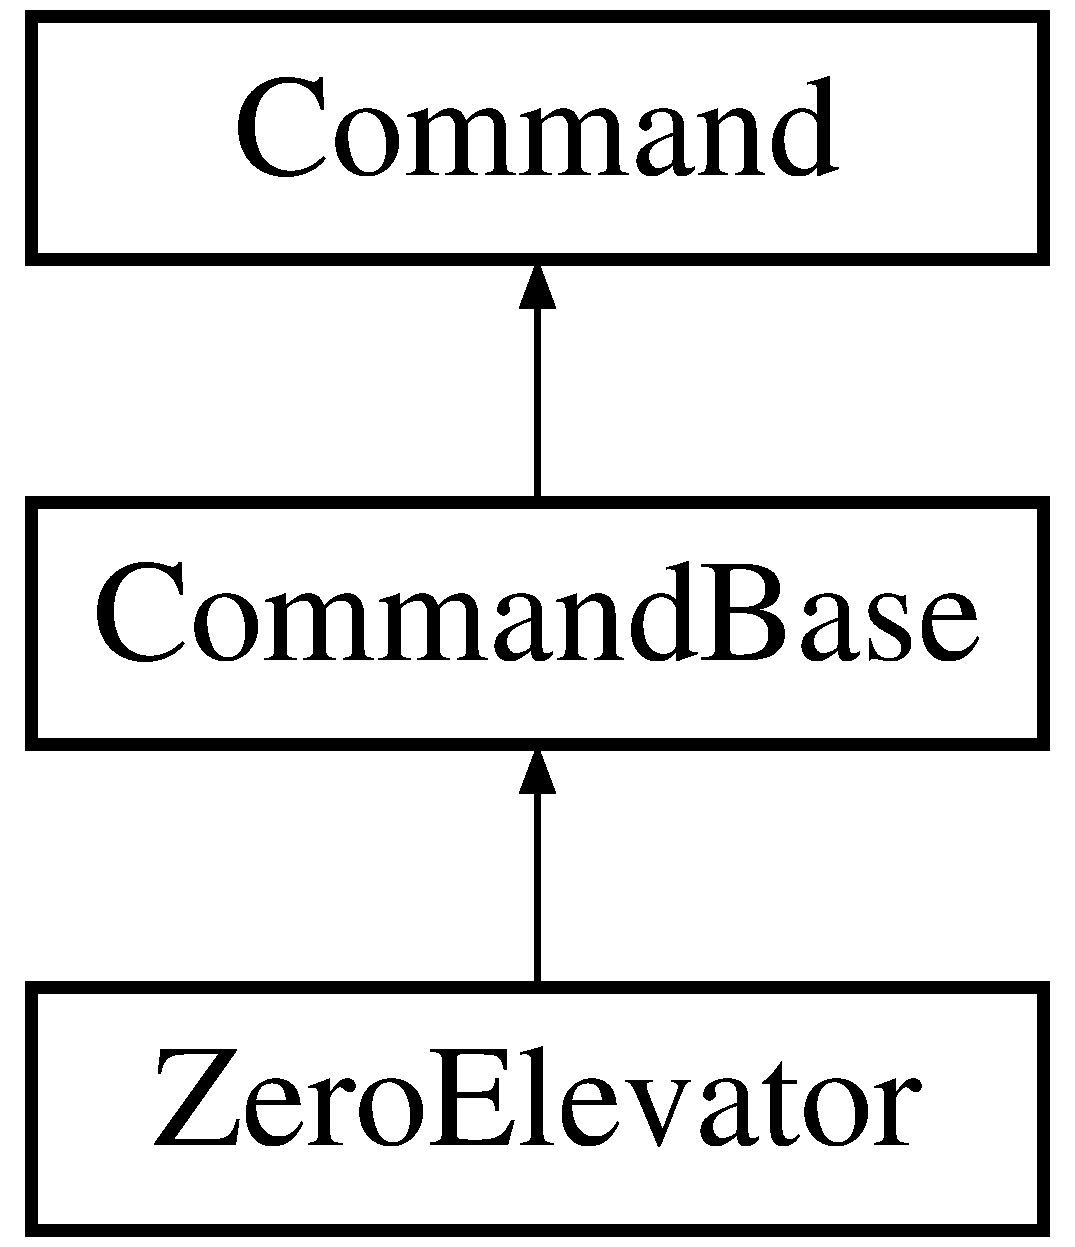
\includegraphics[height=3.000000cm]{class_zero_elevator}
\end{center}
\end{figure}
\subsection*{Public Member Functions}
\begin{DoxyCompactItemize}
\item 
\hypertarget{class_zero_elevator_ade49af7baca93f2819bf15e5d0c28755}{}void {\bfseries Initialize} ()\label{class_zero_elevator_ade49af7baca93f2819bf15e5d0c28755}

\item 
\hypertarget{class_zero_elevator_a302a2c64707964aaa8ed8553dc23b096}{}void {\bfseries Execute} ()\label{class_zero_elevator_a302a2c64707964aaa8ed8553dc23b096}

\item 
\hypertarget{class_zero_elevator_aff4d8ad330e0001ca86a32feb522c9aa}{}bool {\bfseries Is\+Finished} ()\label{class_zero_elevator_aff4d8ad330e0001ca86a32feb522c9aa}

\item 
\hypertarget{class_zero_elevator_a517f0fb6bde77a9558f718556318efb5}{}void {\bfseries End} ()\label{class_zero_elevator_a517f0fb6bde77a9558f718556318efb5}

\item 
\hypertarget{class_zero_elevator_a53b34d8628da07dc943ea634c4192f98}{}void {\bfseries Interrupted} ()\label{class_zero_elevator_a53b34d8628da07dc943ea634c4192f98}

\end{DoxyCompactItemize}
\subsection*{Additional Inherited Members}


\subsection{Detailed Description}
To be ran in auto so that it can be zeroed by the time teleop begins. Code and values still need to be tested. 

The documentation for this class was generated from the following files\+:\begin{DoxyCompactItemize}
\item 
Cyclophosphamide/src/\+Commands/\+Tote\+Lifting/zeroing/Zero\+Elevator.\+h\item 
Cyclophosphamide/src/\+Commands/\+Tote\+Lifting/zeroing/Zero\+Elevator.\+cpp\end{DoxyCompactItemize}

\hypertarget{class_zero_elevator_mag}{}\section{Zero\+Elevator\+Mag Class Reference}
\label{class_zero_elevator_mag}\index{Zero\+Elevator\+Mag@{Zero\+Elevator\+Mag}}


{\ttfamily \#include $<$Zero\+Elevator\+Magnet.\+h$>$}

Inheritance diagram for Zero\+Elevator\+Mag\+:\begin{figure}[H]
\begin{center}
\leavevmode
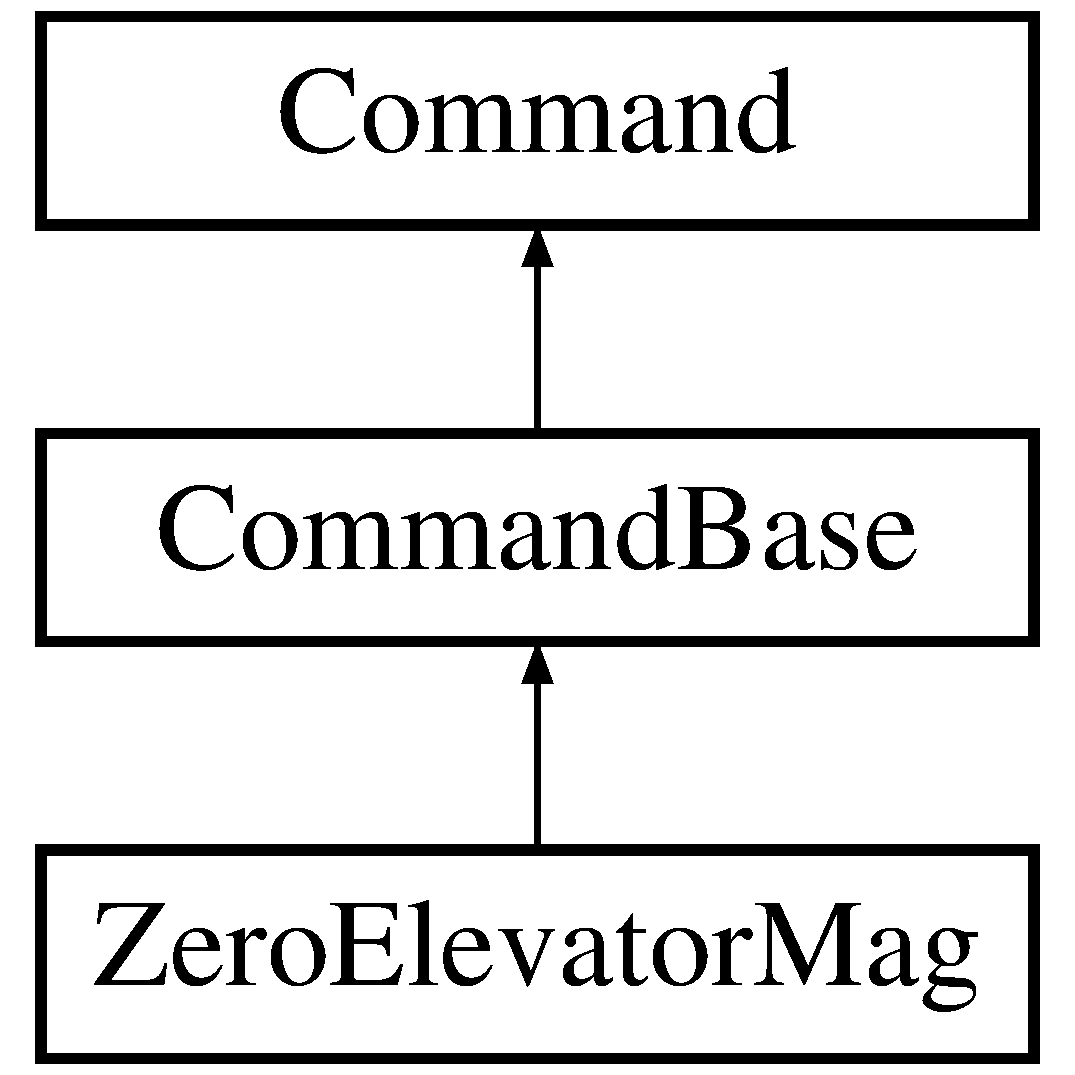
\includegraphics[height=3.000000cm]{class_zero_elevator_mag}
\end{center}
\end{figure}
\subsection*{Public Member Functions}
\begin{DoxyCompactItemize}
\item 
\hypertarget{class_zero_elevator_mag_a02761ea43a4b9eb2b48a04964305dc26}{}void {\bfseries Initialize} ()\label{class_zero_elevator_mag_a02761ea43a4b9eb2b48a04964305dc26}

\item 
\hypertarget{class_zero_elevator_mag_a35313099fa61a059e7b753633bc81a7d}{}void {\bfseries Execute} ()\label{class_zero_elevator_mag_a35313099fa61a059e7b753633bc81a7d}

\item 
\hypertarget{class_zero_elevator_mag_a8fd0506dc8bdf6851e71a8f75cae8d4a}{}bool {\bfseries Is\+Finished} ()\label{class_zero_elevator_mag_a8fd0506dc8bdf6851e71a8f75cae8d4a}

\item 
\hypertarget{class_zero_elevator_mag_a9d284f3178c7bdb3c9208981c245a216}{}void {\bfseries End} ()\label{class_zero_elevator_mag_a9d284f3178c7bdb3c9208981c245a216}

\item 
\hypertarget{class_zero_elevator_mag_a6a911faef39aa93e64e593ce1d316e31}{}void {\bfseries Interrupted} ()\label{class_zero_elevator_mag_a6a911faef39aa93e64e593ce1d316e31}

\end{DoxyCompactItemize}
\subsection*{Additional Inherited Members}


\subsection{Detailed Description}
To be ran in auto so that it can be zeroed by the time teleop begins. Code and values still need to be tested. 

The documentation for this class was generated from the following files\+:\begin{DoxyCompactItemize}
\item 
Cyclophosphamide/src/\+Commands/\+Tote\+Lifting/zeroing/Zero\+Elevator\+Magnet.\+h\item 
Cyclophosphamide/src/\+Commands/\+Tote\+Lifting/zeroing/Zero\+Elevator\+Magnet.\+cpp\end{DoxyCompactItemize}

\hypertarget{class_zero_gyro}{}\section{Zero\+Gyro Class Reference}
\label{class_zero_gyro}\index{Zero\+Gyro@{Zero\+Gyro}}
Inheritance diagram for Zero\+Gyro\+:\begin{figure}[H]
\begin{center}
\leavevmode
\includegraphics[height=3.000000cm]{class_zero_gyro}
\end{center}
\end{figure}
\subsection*{Public Member Functions}
\begin{DoxyCompactItemize}
\item 
\hypertarget{class_zero_gyro_a178a4ffa89e9111068606ac3a57200c6}{}void {\bfseries Initialize} ()\label{class_zero_gyro_a178a4ffa89e9111068606ac3a57200c6}

\item 
\hypertarget{class_zero_gyro_a4f4ea89be6460502d8286423c8cb81cb}{}void {\bfseries Execute} ()\label{class_zero_gyro_a4f4ea89be6460502d8286423c8cb81cb}

\item 
\hypertarget{class_zero_gyro_a427bf7a0e36b00bca9dfcf21fcae6093}{}bool {\bfseries Is\+Finished} ()\label{class_zero_gyro_a427bf7a0e36b00bca9dfcf21fcae6093}

\item 
\hypertarget{class_zero_gyro_ac6c3def0b314afff6d7e48f7811c1bf9}{}void {\bfseries End} ()\label{class_zero_gyro_ac6c3def0b314afff6d7e48f7811c1bf9}

\item 
\hypertarget{class_zero_gyro_af87cb0199efadb4568113aac1b1ba137}{}void {\bfseries Interrupted} ()\label{class_zero_gyro_af87cb0199efadb4568113aac1b1ba137}

\end{DoxyCompactItemize}
\subsection*{Additional Inherited Members}


The documentation for this class was generated from the following files\+:\begin{DoxyCompactItemize}
\item 
Cyclophosphamide/src/\+Commands/\+Drivebase/Zero\+Gyro.\+h\item 
Cyclophosphamide/src/\+Commands/\+Drivebase/Zero\+Gyro.\+cpp\end{DoxyCompactItemize}

%--- End generated contents ---

% Index
\backmatter
\newpage
\phantomsection
\clearemptydoublepage
\addcontentsline{toc}{chapter}{Index}
\printindex

\end{document}
